% !TEX program = xelatex
% !TEX options = -synctex=1 -interaction=nonstopmode -file-line-error --shell-escape "%DOC%"

%----------------------------------------------------------------------------------------
%	PACKAGES AND OTHER DOCUMENT CONFIGURATIONS
%----------------------------------------------------------------------------------------

\documentclass[
  fontsize=10pt,
  twoside=false
  % overfullrule
]{kaobook}

% Choose the language
\usepackage[english]{babel} % Load characters and hyphenation
\usepackage[english=british]{csquotes}	% English quotes

% Load the bibliography package
\usepackage{styles/kaobiblio}
\addbibresource{main.bib} % Bibliography file

% Load mathematical packages for theorems and related environments. NOTE: choose only one between 'mdftheorems' and 'plaintheorems'.
\usepackage{styles/mdftheorems}
%\usepackage{styles/plaintheorems}

\graphicspath{{images/}} % Paths in which to look for images

\makeindex[columns=3, title=Alphabetical Index, intoc] % Make LaTeX produce the files required to compile the index

\makeglossaries % Make LaTeX produce the files required to compile the glossary

\makenomenclature % Make LaTeX produce the files required to compile the nomenclature

% Reset sidenote counter at chapters
%\counterwithin*{sidenote}{chapter}

%%% Then my own packages

\usepackage{fontspec}

\usepackage{mathpartir}

% Trick for current font size
\makeatletter
\newcommand{\currentfontsize}{\fontsize{\f@size}{\f@baselineskip}\selectfont}
\makeatother

% For code higlighting
\usepackage{minted}
\setminted{
	fontsize=\footnotesize,
	encoding=utf8
}
\setmintedinline{fontsize=\currentfontsize}

% HACK: Remove red boxes
% From https://tex.stackexchange.com/questions/343494/minted-red-box-around-greek-characters
\usepackage{etoolbox,xpatch}

\makeatletter
\AtBeginEnvironment{minted}{\dontdofcolorbox}
\def\dontdofcolorbox{\renewcommand\fcolorbox[4][]{##4}}
\xpatchcmd{\inputminted}{\minted@fvset}{\minted@fvset\dontdofcolorbox}{}{}
\xpatchcmd{\mintinline}{\minted@fvset}{\minted@fvset\dontdofcolorbox}{}{}
\makeatother

% Without red boxes: xcode, arduino, abap,
% \usemintedstyle{abap}

\usepackage{stmaryrd}

\usepackage[all]{xy}
\SelectTips{cm}{11}
\CompileMatrices % Caching for xymatrix

% Meta comment
\newcommand\meta[1]{\noindent\textcolor{blue}{\emph{#1}}}
\newcommand\todo{\meta{TODO}}
\def\ms#1{\todo{} (MS) \meta{#1}}
\def\nt#1{\todo{} (NT) \meta{#1}}
\def\tw#1{\todo{} (TW) \meta{#1}}

% Names
\def\name#1{\textsf{#1}\xspace}
\def\Coq{\name{Coq}}
\def\TemplateCoq{\name{TemplateCoq}}
\def\Equations{\name{Equations}}
\def\Andromeda{\name{Andromeda}}
\def\NuPRL{\name{NuPRL}}
\def\Agda{\name{Agda}}
\def\Epigram{\name{EPIGRAM}}
%%% General

\newcommand{\inv}{^{-1}}

% \newcommand{\eg}{e.g.\ }
% \newcommand{\ie}{\emph{i.e.,}\xspace}

\newcommand{\paradot}[1]{\paragraph{#1.}}

\newcommand{\exmark}{\ensuremath{\mathsf{x}}}

%% Proof by cases
\newenvironment{caselist}{%
  \begin{list}{{\it Case}}{}%
}{\end{list}%
}
\newenvironment{subcaselist}{%
  \begin{list}{{\it Subcase}}{}%
}{\end{list}%
}
\newenvironment{subsubcaselist}{%
  \begin{list}{{\it Subsubcase}}{}%
}{\end{list}%
}

\newcommand{\nextcase}{\item~}

%%% Type theory

% Meta
\newcommand{\Ax}{\ensuremath{\mathsf{Ax}}}
\newcommand{\Rl}{\ensuremath{\mathsf{R}}}

% Generic entities
\newcommand{\Ga}{\Gamma}   % a context
\newcommand{\D}{\Delta}   % another context
\newcommand{\E}{\Xi}      % another context
\newcommand{\sbs}{\sigma} % a substitution
\newcommand{\sbt}{\theta} % another substitution
\newcommand{\sbr}{\rho}   % a third substitution

%% Syntax
\newcommand{\bnf}{\ \mathrel{{:}{:}{=}}\ }
\newcommand{\bnfor}{\ \mid\ \ }

%% Contexts
\newcommand{\ctxempty}{\bullet} % empty context
% \newcommand{\ctxextend}[2]{#1, #2} % extended context

%\newcommand{\ctxdom}[1]{\mathsf{dom}(#1)} % the domain of a context

%% Substitution

\newcommand{\sto}{\mathop{\leftarrow}}

% Reduction
\newcommand{\red}{\rightarrowtriangle}
\newcommand{\redl}{\leftarrowtriangle}

%% Marker
\newcommand{\stt}[1]{#1^{\mathsf{s}}}
\newcommand{\fm}[1]{#1^{\mathsf{f}}}


% Type formers
\newcommand{\Prod}[1]{\mathop{\Pi(#1).\ }}                 % dependent product
\newcommand{\Sum}[1]{\mathop{\Sigma(#1).}}               % dependent sum
\newcommand{\Eq}[3]{#2 =_{#1} #3}                        % fibrant equality
\newcommand{\Eqs}[3]{#2 \overset{\mathsf{s}}{=}_{#1} #3} % strict equality
\newcommand{\Ty}[1]{\square_{#1}}
\newcommand{\Un}[1]{\mathsf{U}_{#1}}                      % strict universe
\newcommand{\F}[1]{\mathsf{F}_{#1}}                      % fibrant universe
\newcommand{\Type}{\mathsf{Type}}
\newcommand{\Prop}{\mathsf{Prop}}
\newcommand{\nat}{\mathsf{nat}}
% \newcommand{\zero}{\mathsf{zero}}
\newcommand{\zero}{0}
% \newcommand{\natsucc}{\mathsf{succ}}
\newcommand{\natsucc}{\mathbf{S}}
\newcommand{\natrec}{\mathsf{natrec}}
\newcommand{\bool}{\mathsf{bool}}
\newcommand{\unit}{\mathsf{unit}}

% Inductive types
\newcommand{\Ical}{\mathcal{I}}
\newcommand{\at}[1]{\{#1\}}

% Terms
\newcommand{\lam}[2]{\lambda (#1). #2 .}                        % abstraction
\newcommand{\app}[4]{#1\mathbin{@_{#2.#3}} #4}                  % application
\newcommand{\pair}[4]{\langle #3 ; #4 \rangle_{#1.#2}}          % pair
\newcommand{\pio}[3]{\pi_1^{#1.#2}\ #3}                         % first proj
\newcommand{\pit}[3]{\pi_2^{#1.#2}\ #3}                         % second proj
\newcommand{\idpath}[1]{{\mathsf{idpath}_{#1}}\ }               % identity path
\newcommand{\refl}[1]{{\mathsf{refl}}_{#1}\ }                   % reflexivity
\newcommand{\funexts}[5]
  {\stt{\mathsf{funext}}(#1,#2,#3,#4,#5)}                        % strict funext
\newcommand{\funext}[5]
  {\mathsf{funext}(#1,#2,#3,#4,#5)}                             % fibrant funext
\newcommand{\uip}[5]{\mathsf{uip}(#1,#2,#3,#4,#5)}              % uip
\newcommand{\J}[6]{\mathsf{J}(#1,#2,#3,#4,#5,#6)}               % the J elim
\newcommand{\Js}[6]{\mathsf{J}^{\mathsf{s}}(#1,#2,#3,#4,#5,#6)} % the J elim
\newcommand{\ttrue}{\mathsf{true}}
\newcommand{\ffalse}{\mathsf{false}}
\newcommand{\tif}[4]{\mathsf{if}\ #1\ \mathsf{return}\ #2\ \mathsf{then}\ #3\ \mathsf{else}\ #4}
\newcommand{\notfunext}{\mathsf{notfunext}}
\newcommand{\Notfunext}{\mathsf{NotFunExt}}
\newcommand{\tunit}{\mathsf{())}}

% Pattern-matching
\newcommand{\matchs}{\mathsf{match}}
\newcommand{\patt}[2]{\mid #1 \Longrightarrow #2}
\newcommand{\match}[3]{%
  \begin{array}{l}%
    \matchs\ #1 \\ \mathsf{return}\ #2\ \mathsf{with} \\ #3 \\ \mathsf{end}%
  \end{array}%
}

% Vectors
\newcommand{\av}{\vec{a}}
\newcommand{\bv}{\vec{b}}
\newcommand{\iv}{\vec{i}}
\newcommand{\pv}{\vec{p}}
\newcommand{\sv}{\vec{s}}
\newcommand{\Av}{\vec{A}}
\newcommand{\Iv}{\vec{I}}
\newcommand{\Nv}{\vec{N}}
\newcommand{\Pv}{\vec{P}}
\newcommand{\Vv}{\vec{V}}
\newcommand{\Xv}{\vec{X}}
\newcommand{\Yv}{\vec{Y}}

% Judgments
\newcommand{\isctx}[1]{\vdash #1}          % well formed context
\newcommand{\istype}[2]{#1 \vdash #2}      % well formed type
\newcommand{\isterm}[3]{#1 \vdash #2 : #3} % well formed term

\newcommand{\eqtype}[3]{#1 \vdash #2 \equiv #3}      % equal types
\newcommand{\eqterm}[4]{#1 \vdash #2 \equiv #3 : #4} % equal terms

\newcommand{\isjg}[2]{#1 \vdash \mathcal{#2}} % arbitrary judgment

% Ext. judgments
\newcommand{\xisctx}[1]{\vdash_{\exmark} #1}          % well formed context
\newcommand{\xistype}[2]{#1 \vdash_{\exmark} #2}      % well formed type
\newcommand{\xisterm}[3]{#1 \vdash_{\exmark} #2 : #3} % well formed term

\newcommand{\xeqtype}[3]{#1 \vdash_{\exmark} #2 \equiv #3}      % equal types
\newcommand{\xeqterm}[4]{#1 \vdash_{\exmark} #2 \equiv #3 : #4} % equal terms

\newcommand{\xisjg}[2]{#1 \vdash_{\exmark} \mathcal{#2}} % arbitrary judgment

% Translation
\newcommand{\transl}[1]{\llbracket #1 \rrbracket}
\newcommand{\So}{\mathsf{S}}
\newcommand{\HTS}{\mathsf{HTS}}
\newcommand{\Gb}{\overline{\Ga}}
\newcommand{\Db}{\overline{\D}}
\newcommand{\Ab}{\overline{A}}
\newcommand{\Bb}{\overline{B}}
\newcommand{\Tb}{\overline{T}}
\newcommand{\Pb}{\overline{P}}
\newcommand{\eb}{\overline{e}}
\newcommand{\jg}{\mathcal{J}}
\newcommand{\jgb}{\overline{\jg}}
\newcommand{\ub}{\overline{u}}
\newcommand{\vb}{\overline{v}}
\newcommand{\wb}{\overline{w}}
\newcommand{\pb}{\overline{p}}
\newcommand{\tb}{\overline{t}}
\newcommand{\fb}{\overline{f}}
\newcommand{\gb}{\overline{g}}

\newcommand{\transpo}[1]{#1_*}
\newcommand{\otransport}[4]{\mathsf{transport}'_{#1,#2}(#3,#4)}

\newcommand{\translitivity}[2]{\mathsf{transitivity}(#1,#2)}
\newcommand{\otransitivity}[2]{\mathsf{transitivity}'(#1,#2)}

% Operations
\newcommand{\nmax}[2]{\mathsf{max}(#1,#2)}

% Notations
\newcommand{\Heqs}{\cong}
\newcommand{\Heq}[4]{#2 \mathrel{{}_{#1}{\Heqs}_{#3}} #4}
\newcommand{\ir}{\sqsubset}
\newcommand{\Pack}[2]{\mathsf{Pack}\ #1\ #2}
% \newcommand{\ProjO}[3]{\mathsf{Proj}_1\ #1\ #2\ #3}
% \newcommand{\ProjT}[3]{\mathsf{Proj}_2\ #1\ #2\ #3}
% \newcommand{\ProjE}[3]{\mathsf{Proj}_e\ #1\ #2\ #3}
\newcommand{\ProjO}[1]{\mathsf{Proj}_1\ #1}
\newcommand{\ProjT}[1]{\mathsf{Proj}_2\ #1}
\newcommand{\ProjE}[1]{\mathsf{Proj}_\mathsf{e}\ #1}
\newcommand{\llift}[3]{#3 {[#1_1]}^{#2}}
\newcommand{\rlift}[3]{#3 {[#1_2]}^{#2}}
% \newcommand{\lo}[1]{\llift{}{}{#1}}
% \newcommand{\ro}[1]{\rlift{}{}{#1}}
\newcommand{\lo}[1]{#1 \upharpoonleft}
\newcommand{\ro}[1]{#1 \upharpoonright}
\newcommand{\Gp}{\Ga_\mathsf{p}}


% Links to the repository

% For anonymity we should remove the links
\newcommand{\repoURL}{https://github.com/TheoWinterhalter/ett-to-itt/blob/master/theories/}
\newcommand{\rpath}[1]{\href{{\repoURL #1}}{#1}}
% \newcommand{\rpath}[1]{\path{#1}}
 % TODO Integrate into macros and factorise

% Customising margin citations
\renewcommand{\formatmargincitation}[1]{%
	\color{Gray!50} \parencite{#1}: \citeauthor*{#1} (\citeyear{#1}), \citetitle{#1}\\%
}

% Font fallback
\usepackage{newunicodechar}
\newfontfamily{\fallbackmonofont}{Symbola}[Scale=MatchLowercase]
\DeclareTextFontCommand{\textfallbackmono}{\fallbackmonofont}
\newcommand{\fallbackcharmono}[2][\textfallbackmono]{%
    \newunicodechar{#2}{#1{#2}}%
}
\fallbackcharmono{⊗}
\fallbackcharmono{⊩}
\fallbackcharmono{⨶}
\fallbackcharmono{⊨}
\fallbackcharmono{⨷}
\fallbackcharmono{⊕}

%----------------------------------------------------------------------------------------

\begin{document}

% \setmainfont[Ligatures=TeX]{Fira Math Light}
\setmainfont[
	Ligatures=TeX,
	% UprightFont = ,
	ItalicFont = Fira Sans Light Italic,
	% SmallCapsFont = ,
	BoldFont = Fira Sans,
	BoldItalicFont = Fira Sans Italic
]{Fira Sans Light}
% \setsansfont[Ligatures=TeX]{Fira Sans}
\setmonofont[Ligatures=TeX]{Fira Mono}
% \setmonofont[Ligatures=TeX]{Symbola}

%----------------------------------------------------------------------------------------
%	BOOK INFORMATION
%----------------------------------------------------------------------------------------

\titlehead{Some text}
\subject{PhD Thesis}

\title{Formalisation and Meta-Theory of Type Theory}
\subtitle{Customise this page according to your needs}

\author{Théo Winterhalter}

\date{\today}

\publishers{An Awesome Publisher}

%----------------------------------------------------------------------------------------

\frontmatter % Denotes the start of the pre-document content, uses roman numerals

%----------------------------------------------------------------------------------------
%	OPENING PAGE
%----------------------------------------------------------------------------------------

%\makeatletter
%\extratitle{
%	% In the title page, the title is vspaced by 9.5\baselineskip
%	\vspace*{9\baselineskip}
%	\vspace*{\parskip}
%	\begin{center}
%		% In the title page, \huge is set after the komafont for title
%		\usekomafont{title}\huge\@title
%	\end{center}
%}
%\makeatother

%----------------------------------------------------------------------------------------
%	COPYRIGHT PAGE
%----------------------------------------------------------------------------------------

\makeatletter
\uppertitleback{\@titlehead} % Header

\lowertitleback{
	\textbf{Disclaimer}\\
	You can edit this page to suit your needs. For instance, here we have a no copyright statement, a colophon and some other information. This page is based on the corresponding page of Ken Arroyo Ohori's thesis, with minimal changes.

	\medskip

	\textbf{No copyright}\\
	\cczero\ This book is released into the public domain using the CC0 code. To the extent possible under law, I waive all copyright and related or neighbouring rights to this work.

	To view a copy of the CC0 code, visit: \\\url{http://creativecommons.org/publicdomain/zero/1.0/}

	\medskip

	\textbf{Colophon} \\
	This document was typeset with the help of \href{https://sourceforge.net/projects/koma-script/}{\KOMAScript} and \href{https://www.latex-project.org/}{\LaTeX} using the \href{https://github.com/fmarotta/kaobook/}{kaobook} class.

	The source code of this book is available at:\\\url{https://github.com/fmarotta/kaobook}

	(You are welcome to contribute!)

	\medskip

	\textbf{Publisher} \\
	First printed in May 2019 by \@publishers
}
\makeatother

%----------------------------------------------------------------------------------------
%	DEDICATION
%----------------------------------------------------------------------------------------

\dedication{
	Figure something to put here or remove it altogether.\\
	\flushright -- Myself
}

%----------------------------------------------------------------------------------------
%	OUTPUT TITLE PAGE AND PREVIOUS
%----------------------------------------------------------------------------------------

% Note that \maketitle outputs the pages before here

% If twoside=false, \uppertitleback and \lowertitleback are not printed
% To overcome this issue, we set twoside=semi just before printing the title pages, and set it back to false just after the title pages
\KOMAoptions{twoside=semi}
\maketitle
\KOMAoptions{twoside=false}

%----------------------------------------------------------------------------------------
%	PREFACE
%----------------------------------------------------------------------------------------

%\input{chapters/preface.tex}

%----------------------------------------------------------------------------------------
%	TABLE OF CONTENTS & LIST OF FIGURES/TABLES
%----------------------------------------------------------------------------------------

\begingroup % Local scope for the following commands

% Define the style for the TOC, LOF, and LOT
%\setstretch{1} % Uncomment to modify line spacing in the ToC
%\hypersetup{linkcolor=blue} % Uncomment to set the colour of links in the ToC
\setlength{\textheight}{23cm} % Manually adjust the height of the ToC pages

% Turn on compatibility mode for the etoc package
\etocstandarddisplaystyle % "toc display" as if etoc was not loaded
\etocstandardlines % "toc lines as if etoc was not loaded

\tableofcontents % Output the table of contents

\listoffigures % Output the list of figures

% Comment both of the following lines to have the LOF and the LOT on different pages
\let\cleardoublepage\bigskip
\let\clearpage\bigskip

\listoftables % Output the list of tables

\endgroup

%----------------------------------------------------------------------------------------
%	MAIN BODY
%----------------------------------------------------------------------------------------

\mainmatter % Denotes the start of the main document content, resets page numbering and uses arabic numbers
\setchapterstyle{kao} % Choose the default chapter heading style

% \setchapterpreamble[u]{\margintoc}
\chapter{Introduction}
\labch{intro}

\todo{Nicolas: Speak about ``derivation checking''. Where? How?}

Type theory places itself at the interface between programming and formal logic,
feeding off and nourishing both worlds. Proof assistants can be built on it,
making them full-fledged programming languages as well.

My main interest lies in the study of type theory while relying on the tools it
provides: I study type theory \emph{in} type theory.
\todo{Just keep writing what I want to put in here and then write it}

\paradot{Contributions}
My contributions will mainly be found in \arefpart{elim-reflection} and
\arefpart{coq-in-coq} corresponding to the following published
articles~\sidecite{winterhalter:hal-01849166,sozeau2019coq,sozeau:hal-02167423}.
While the chapters before these two parts are mainly introductory and
corresponding to a rough state-of-the-art, they actually contain other
contributions, namely work I did with Andrej Bauer on the cardinal model
in \nrefch{models} that we didn't publish, and work I did with Andrej Bauer
and Philipp Haselwarter on formalising type theory called
\ftt~\sidecite{formaltypetheory} and that I present briefly in
\nrefch{formalisation}.

\paradot{Outline}
\todo{TODO}

\pagelayout{wide} % No margins
\addpart{Proofs, Types and Programs}
\pagelayout{margin} % Restore margins

% \setchapterpreamble[u]{\margintoc}
\chapter{Proof theory}
\labch{proof-theory}

My work is done in the wide domain of proof theory. Proof theorists are
interested in the way to prove things, in the `proof' object itself, \eg we
might want to check that a proof uses some specific rules of deduction.
We may also want to prove that a system is not contradictory, \ie that it does
not entail both an assertion and its negation.
This allows us to understand more about proof reuse, about transposition of a
property to another system, or about some intrinsinc properties of the proof
itself. The study of proofs also allows to define clear systems outlining
formally what a proof is and when it is valid. This leads to the notion of
certificate that one can check independently. The epitome of this is the ability
to write proofs that are checkable by a computer, shifting the trust one needs
to put within every proof, to the system which validates them all.

\section{How to prove something}

\subsection{A social construct?}

Before we start proving something, we must know precisely what it is we want to
prove. In informal mathematics, the statement will be a sentence, involving
concepts that the writer and reader agree on. The proof then consists in a
sequence of sentences and argument that convince the same readers.

For instance, the Pythagorean theorem states that
``the area of the square whose side is the hypothenuse of a right triangle is
equal to the sum of the areas of the squares on the other two sides.''

With this definition, a proof is a subjective concept, it depends on the
reader's capacity to understand and potentially fill the gap themselves about
understood statements and properties. It also usually involves a fair bit of
\emph{trusting}: you may not understand a proof, but will believe in
the common effort of the community to verify the proof or, even better,
reproduce it.
As such, \emph{consensus} seems key in the scientific community.

One way to reach consensus much faster is to have statements and proofs really
precise and unambiguous, described in formal systems. This approach still has
shortcomings, will all readers check every tiny detail of the proof once it is
laid out extensively? This runs the risk of having the \emph{idea} lost in a
sea of information.
To me, this calls for computer-verified proofs---and maybe even automated or
computer aided proofs---coming with paper proofs exposing the ideas
so that the reader can focus on the interesting part of
the proof while trusting only the tool and not the human that used it.

Even then, there is room for question on whether this really constitutes a
proof.
For instance, how \emph{hard} is it for the computer to \emph{see} that the
proof is indeed correct? One definition would be to say, as long as it takes
a finite amount of time, it is good, but if it takes ages, we will not have any
certainty. In \sidecite{de1991plea}, de Bruijn suggests that a proof should be
self-evident. You should not have to think for hours before seeing that is
indeed correct, and the same holds for computers.

In the remainder of the section I will address the way we \emph{write}
statements and proofs.

\subsection{Formal statements}

\marginnote[0.2cm]{
  Since I want to be as general as possible, this talk about formal statements
  will be pretty informal.
}
What do formal statements look like? Probably something like
\[
  \forall n \in \mathbb{N}. \exists m \in \mathbb{R}.
  f(n) = \mathsf{e}^{\phi(m)} \wedge g(n) > m
\]
It involves defined symbols, and logical connectives to make something precise.
In particular you will note the universal (\(\forall\)) and existential
(\(\exists\)) quantifiers, equality (\(=\)), logical conjunction (\(\wedge\))
and a comparison operator (\(>\)).
We can assume \(\mathbb{N}\), \(\mathbb{R}\), \(f\), \(g\), \(h\), \(\phi\) and
\(e\) to be defined prior to the statement (using similar formalism).

To define this, we give a syntax of propositions, mutually with a syntax of
sets on which we want to quantify. Because equality can mention elements however
we also have to provide a syntax for those, and maybe one for function symbols.
\marginnote[0.7cm]{
  Here \(P \to Q\) denotes `\(P\) implies \(Q\)', often written
  \(P \Longrightarrow Q\). In my domain things are different and we use a single
  arrow.
}
\[
  \begin{array}{rrl}
    P, Q &\bnf& \top \bnfor \bot \bnfor P \wedge Q \bnfor P \vee Q
    \bnfor P \to Q \\
    &\bnfor& \forall x \in E. P \bnfor \exists x \in E. P \bnfor u = v \\
    E &\bnf& \mathbb{N} \bnfor \mathbb{R} \bnfor \dots \\
    u, v &\bnf& x \bnfor \mathsf{e}^u \bnfor u + v \bnfor f(u) \bnfor \dots \\
    f, g, h &\bnf& \dots
  \end{array}
\]

\marginnote[0.5cm]{
  Parentheses are not part of the syntax but are there to lift any ambiguity
  and distinguish \(P \wedge (Q \vee R)\) from \((P \wedge Q) \vee R\)
  for example.
}
This presentation of syntax is called \acrfull{BNF} and it says that there are
expressions that we will write with \(P\) or \(Q\) that can be either \(\top\)
or \(\bot\) or \(P \wedge Q\) where \(P\) and \(Q\) are both of the same form,
and so on.
For instance, \(\bot \wedge (\top \vee (\top \to \bot))\) is one such
expression.

Here \(P,Q\) are propositions, \(E\) stands for a set, \(u,v\) are mathematical
expressions whereas \(f,g,h\) are function symbols.

Logical connectives (\(\wedge, \vee, \forall\), \dots) and operations
(\(+, \times\), \dots) are the building blocks of statements, as such we call
them \emph{constructors}.

Coming up with a correct syntax like those can be pretty painful so formalisms
tend to be as minimal as possible, the other advantage being that it is much
easier to reason on the statements when there are not hundreds of syntactical
constructs.

Of course, giving a syntax of statements is not enough. We must give these
symbols a semantics (\ie a meaning) to know what it means to prove them.
For instance, we might want to sepcify that the symbol \(+\) has the properties
which are expected of addition.

\subsection{Inference rules}

We need to define what it means to prove a statement given some hypotheses.
For instance we have
\[
  A, B \vdash A \wedge B
\]
to denote the fact that \(A\) and \(B\) as hypotheses, \emph{entail} the
proposition \(A \wedge B\) (read `\(A\) \emph{and} \(B\)').
\marginnote[0.2cm]{
  There are also settings where several propositions appear on the right-hand
  side: \(A, B \vdash C, D\) means that assuming \(A\) and \(B\) then either
  \(C\) or \(D\) hold.
}
This is called a \emph{judgement}: \(A, B, C \vdash D\) means that,
\emph{assuming} \(A\), \(B\) \emph{and} \(C\), then \(D\) holds.
\[
  \begin{array}{rcl}
    \Ga, \D &\bnf& \ctxempty \bnfor \Ga, P \\
    \mathcal{J} &\bnf& \Ga \vdash P
  \end{array}
\]
We can now move on to the notion of \emph{inference} rule. They are what defines
the logic that we consider, they dictate what judgements can be
\emph{derived}---\ie proven---and how.
The simplest of rules usually is the so-called \emph{axiom} rule stating that
assuming \(A\), you can prove \(A\).
% \marginnote[-0.3cm]{
%   Alternatively we could consider
%   \[
%     \infer
%       {A \in \Ga}
%       {\Ga \vdash A}
%   \]
% }
\[
  \infer
    { }
    {A \vdash A}
\]
or more generally
\[
  \infer
    {A \in \Ga}
    {\Ga \vdash A}
\]
The line separates one judgement below, the conclusion, to one, several or
possibly no judgements above. They represent requirements to conclude the below
part. In this case, one does not need to assume anything to conclude that \(A\)
entails \(A\). The condition \(A \in \Ga\) is not a judgement itself but really
a side condition.
Going back to conjunction, the rule\sidenote{It is actually one of many possible
rules. It all depends on the logic.} to prove one is the following.
\[
  \infer
    {
      \Ga \vdash A \\
      \Ga \vdash B
    }
    {\Ga \vdash A \wedge B}
\]
That is to say, to prove \(A \wedge B\) (under hypotheses \(\Ga\)), it
\emph{suffices} to prove \(A\) and \(B\) (under the same hypotheses).
This is called an \emph{introduction} rule because it allows us to introduce a
connective in the conclusion.
\marginnote[0.3cm]{
  Once again, this is one of many ways to proceed.
  This setting corresponds to \emph{natural deduction} and was introduced by
  Gentzen; he also introduced \emph{sequent calculus} where there are no
  elimination rules, but introduction rules on the left and on the right.
}
Sometimes, we want to be able to conclude something from a complex assumption
like \(A \wedge B\), this is instead called an \emph{elimination} rule.
\begin{mathpar}
  \infer
    {\Ga \vdash A \wedge B}
    {\Ga \vdash A}
  %

  \infer
    {\Ga \vdash A \wedge B}
    {\Ga \vdash B}
  %
\end{mathpar}
If you can prove \(A \wedge B\) then you can prove \(A\) (you can also prove
\(B\) but that is another rule).
We then have similar rules for disjunction
(\(A \vee B\) reads `\(A\) \emph{or} \(B\)').
\marginnote[0.5cm]{
  To prove \(A \vee B\) you only need to prove either \(A\) or \(B\), hence the
  two introduction rules. On the contrary if you want to prove \(P\) knowing
  \(A \vee B\), you have to provide a proof for the two different cases: either
  \(A\) holds, or \(B\) holds, in both instances \(P\) should hold.
}
\begin{mathpar}
  \infer
    {\Ga \vdash A}
    {\Ga \vdash A \vee B}
  %

  \infer
    {\Ga \vdash B}
    {\Ga \vdash A \vee B}
  %

  \infer
    {
      \Ga \vdash A \vee B \\
      \Ga, A \vdash P \\
      \Ga, B \vdash P
    }
    {\Ga \vdash P}
  %
\end{mathpar}

Amongst the most important rules are those related to implication.
\begin{mathpar}
  \infer
    {\Ga, A \vdash B}
    {\Ga \vdash A \to B}
  %

  \infer
    {
      \Ga \vdash A \to B \\
      \Ga \vdash A
    }
    {\Ga \vdash B}
  %
\end{mathpar}
They are interesting because they show a level of interaction between the
entailement and the implication. To prove that \(A \to B\), you only assume
\(A\) and show \(B\). Moreover, if you know \(A \to B\) and \(A\), then you
have \(B\). This last rule is called the \emph{modus ponens}, that is the
elimination of the implication.

% Because of this, it might seem like implication (\(\to\)), entailement
% (\(\vdash\)) and inference (---) are three forms of logical implication.
% They \emph{are}, but at different levels.

\section{Proof frameworks}

There are many proof frameworks and logics and I will not review all of them,
but I will present the most relevant ones to the rest of my work.

\subsection{Classical logic}

Classical logic is the logic most people have in mind where any proposition is
either ``true'' or ``false'' (but not either provable or provably
contradictory).
% Gentzen describe it in a sequent calculus called
% \LK~\sidecite{gentzen1935untersuchungen}.
Gentzen describes a natural deduction system called
\NK~\sidecite{gentzen1935untersuchungen}.

The syntax is given by
\[
  \begin{array}{rrl}
    P, Q, A, B &\bnf& \top \bnfor \bot \bnfor P \wedge Q \bnfor P \vee Q
    \bnfor P \to Q \bnfor \neg P \\
    \Ga, \D &\bnf& \ctxempty \bnfor \Ga, P \\
    \mathcal{J} &\bnf& \Ga \vdash \D
  \end{array}
\]
which corresponds to \emph{propositional logic}.
Notice how the right-hand side of judgements contains a context, \ie a list of
propositions, rather than just one as we previously saw.

I will give the rules in two separate bundle.
We first have the logical rules---\ie that pertain to the logical constructors
of propositional logic:
\marginnote[1cm]{
  Next to the rules I write their name in parentheses.
  \(ax\) stands for `axiom'.
  The \(I\)s and \(E\)s in rules indicate whether each rule is an introduction
  rule or an elimination rule.
}
\begin{mathpar}
  \infer
    {A \in \Ga}
    {\Ga \vdash A}
  (ax)

  \infer
    {
      \Ga \vdash A \\
      \Ga \vdash B
    }
    {\Ga \vdash A \wedge B}
  (\wedge I)

  \infer
    {\Ga \vdash A \wedge B}
    {\Ga \vdash A}
  (\wedge E_1)

  \infer
    {\Ga \vdash A \wedge B}
    {\Ga \vdash B}
  (\wedge E_2)

  \infer
    {\Ga \vdash A, B, \D}
    {\Ga \vdash A \vee B, \D}
  (\vee I)

  \infer
    {\Ga \vdash A \vee B, \D}
    {\Ga \vdash A, B, \D}
  (\vee E)

  \infer
    {\Ga, A \vdash B, \D}
    {\Ga \vdash A \to B, \D}
  (\to I)

  \infer
    {
      \Ga \vdash A \to B, \D \\
      \Xi \vdash A, \Theta
    }
    {\Ga, \Xi \vdash \D, \Theta}
  (\to E)

  \infer
    {\Ga, A \vdash \D}
    {\Ga \vdash \neg A, \D}
  (\neg I)

  \infer
    {
      \Ga \vdash \neg A, \D \\
      \Xi \vdash A, \Theta
    }
    {\Ga, \Xi \vdash \D, \Theta}
  (\neg E)

  \infer
    { }
    {\vdash \top}
  (\top I)

  \infer
    {\Ga \vdash \D}
    {\Ga \vdash \bot, \D}
  (\bot I)

  \infer
    {\Ga \vdash \bot, \D}
    {\Ga \vdash \D}
  (\bot E)
\end{mathpar}

The rest are structural rules that allow us to weaken the hypotheses (\ie add
a new, unused hypothesis in the context) or the conclusion, or reorder
propositions and remove duplicates.
\marginnote[1cm]{
  \(W\) stands for weakening, \(C\) for contraction and \(P\) for permutation
  while \(L\) and \(R\) stand for left and right.
}
\begin{mathpar}
  \infer
    {\Ga \vdash \D}
    {\Ga, A \vdash \D}
  (WL)

  \infer
    {\Ga \vdash \D}
    {\Ga \vdash A, \D}
  (WR)

  \infer
    {\Ga, A, A \vdash \D}
    {\Ga, A \vdash \D}
  (CL)

  \infer
    {\Ga \vdash A, A, \D}
    {\Ga \vdash A, \D}
  (CR)

  \infer
    {\Ga, A, B, \Xi \vdash \D}
    {\Ga, B, A, \Xi \vdash \D}
  (PL)

  \infer
    {\Ga \vdash \D, A, B, \Theta}
    {\Ga \vdash \D, B, A, \Theta}
  (PR)
\end{mathpar}

\NK is classical because we can derive the \acrfull{LEM} from it.
\begin{mathpar}
  \infer*[Right=\(\vee I\)]
    {
      \infer*[Right=\(PR\)]
        {
          \infer*[Right=\(\neg I\)]
            {
              \infer*[Right=\(ax\)]
                { }
                {P \vdash P}
            }
            {\vdash \neg P, P}
        }
        {\vdash P, \neg P}
    }
    {\vdash P \vee \neg P}
\end{mathpar}

\NK also features double negation elimination:
\[
  \infer*[Right=\((\to I)\)]
    {
      \infer*[Right=\((\neg E)\)]
        {
          \infer*[Right=\((ax)\)]
            { }
            {\neg \neg P \vdash \neg \neg P}
          \\
          \infer*[Right=\((\neg I)\)]
            {
              \infer*[Right=\((ax)\)]
                { }
                {P \vdash P}
            }
            {\vdash \neg P, P}
        }
        {\neg \neg P \vdash P}
    }
    {\vdash \neg \neg P \to P}
\]

\subsection{Intuitionistic logic}

Intuitionistic logic does not abide by the \acrlong{LEM}, so its treatment of
negation is a bit different so that double negation cannot be eliminated as
above. As such we define \NJ in natural deduction, on the same syntax of
propositional logic. The main difference is that we revert to only one
propositions on the right-hand side of judgements.
It is pretty similar to \NK.
\begin{mathpar}
  \infer
    {A \in \Ga}
    {\Ga \vdash A}
  (ax)

  \infer
    {
      \Ga \vdash A \\
      \Ga \vdash B
    }
    {\Ga \vdash A \wedge B}
  (\wedge I)

  \infer
    {\Ga \vdash A \wedge B}
    {\Ga \vdash A}
  (\wedge E_1)

  \infer
    {\Ga \vdash A \wedge B}
    {\Ga \vdash B}
  (\wedge E_2)

  \infer
    {\Ga \vdash A}
    {\Ga \vdash A \vee B}
  (\vee I_1)

  \infer
    {\Ga \vdash B}
    {\Ga \vdash A \vee B}
  (\vee I_2)

  \infer
    {
      \Ga \vdash A \vee B \\
      \Ga, A \vdash C \\
      \Ga, B \vdash C
    }
    {\Ga \vdash C}
  (\vee E)

  \infer
    {\Ga, A \vdash B}
    {\Ga \vdash A \to B}
  (\to I)

  \infer
    {
      \Ga \vdash A \to B \\
      \Ga \vdash A
    }
    {\Ga \vdash B}
  (\to E)

  \infer
    {\Ga, A \vdash \bot}
    {\Ga \vdash \neg A}
  (\neg I)

  \infer
    {
      \Ga \vdash \neg A \\
      \Ga \vdash A
    }
    {\Ga \vdash \bot}
  (\neg E)

  \infer
    { }
    {\Ga \vdash \top}
  (\top I)

  \infer
    {\Ga \vdash \bot}
    {\Ga \vdash A}
  (\bot E)
\end{mathpar}

The structural rules are only happening on the left now since there is nothing
to rearrange on the right.
\begin{mathpar}
  \infer
    {\Ga \vdash B}
    {\Ga, A \vdash B}
  (W)

  \infer
    {\Ga, A, A \vdash B}
    {\Ga, A \vdash B}
  (C)

  \infer
    {\Ga, A, B, \D \vdash A}
    {\Ga, B, A, \D \vdash A}
  (P)
\end{mathpar}

This logic is constructive in that, from every proof derivation one can extract
a proof where the last rule is an introduction rule.
For instance, every proof of \(A \vee B\) must contain either a proof of \(A\)
or a proof of \(B\).
This is obtained by a process known as \emph{cut-elimination} which removes all
occurrences of the modus ponens \((\to E)\) rule in a derivation, showing at the
same time that it is \emph{admissible} or redundant.

\subsection{Mechanised proofs}

Once we have a formal logic, it makes sense to \emph{teach} its rules to a
computer to use it for what we call \emph{mechanised proofs}.
We nowadays have many of those, be it under the name \emph{proof assistants} or
\emph{automated theorem provers}.

\paragraph{Automated theorem provers} are tools that will take statements as
inputs and attempt to prove or disprove them, sometimes taking hints from the
user when stuck.
They are very attractive because the user usually does not have to learn about
the logic involved, just trust that it \emph{works}\sidenote{Ideally that it is
consistent}. However it can be a hassle when they fail to prove or disprove
something and the user has to figure out the right way to state things so that
the tool manages to progress.

\paragraph{Proof assistants} require more work from the part of the user but are
usually more malleable and robust. They constitute a framework in which the user
can state and prove lemmata. Again there are several proof assistants: \IsaHOL
is one of the most commonly used and based on
\acrfull{HOL}~\sidecite[-1.35cm]{10.5555/1791547}, but I am more  familiar with
proof assistants based on type theory such as \Coq~\sidecite[-1cm]{coq} and
\Agda~\sidecite[-0.4cm]{norell2007towards}.
The next introductory chapters will focus on this notion of proof framework.

\section{Limitations: Gödel's incompleteness theorems}

When you have a proof framework or logic, there are two main things you want to
know about it:
\begin{itemize}
  \item Is it \emph{consistent}? An inconsistent system is one in which we can
  prove that an assertion and its negation.
  \item Is it \emph{complete}? That is, are all propositions either provable
  or provably contradictory (\ie the negation is provable)?
\end{itemize}

Consistency can be reformulated equivalently as the absence of proof of false
\(\bot\).
Completeness is not to be confused with the \acrshort{LEM} which gives a proof
of \(P \vee \neg P\) for each \(P\) but not a proof of either \(P\) or
\(\neg P\) for every \(P\).

Ideally we would want our favourite system to enjoy \emph{both} of these
properties, the proof of which would be conducted in the very same system.
In 1931~\sidecite{godel1931formal} Gödel shattered all hopes of ever
accomplishing that.

\begin{theorem}[Gödel's first incompleteness theorem]
  Every consistent formal system that supports arithmetic is incomplete.
\end{theorem}

\marginnote[1cm]{
  Some people still work in inconsistent logics so let us stress the
  \emph{usually}.
}
This means, that, except in very small systems, consistency and completeness
cannot hold at the same time. Usually we go with consistency because
inconsistent systems are trivially complete (every property is provable) and not
of much interest.

\begin{theorem}[Gödel's second incompleteness theorem]
  Every consistent formal system that supports arithmetic cannot prove its
  own consistency.
\end{theorem}
A system that is able to prove itself consistent is actually inconsistent.
This means that we have to rely on the scientific \emph{consensus} I mentioned
ealier, because the system in which you prove one system consistent is stronger
and needs to be trusted as well.

In both these theorems we talk about the fact that the theory should support
arithmetic for them to apply. By arithmetic we mean Robinson
arithmetic~\sidecite{robinson1950essentially} rather than Peano arithmetic,
as proved in~\sidecite[0.7cm]{bezboruah1976godel}.
It is an axiomatisation of a set \(\mathbb{N}\) with distinguished member
\(0\) and a successor (unary) operation on \(\mathbb{N}\) written \(\So\).
Moreover it features two binary operations called addition and multiplication
written with infix notations \(+\) and \(\times\).
The axioms are the following.
\[
  \begin{array}{ll}
    \forall x.& \So\ x \not= 0 \\
    \forall x\ y.& \So\ x = \So\ y \to x = y \\
    \forall x.& x = 0 \vee \exists y.\ x = \So\ y \\
    \forall x.& x + 0 = x \\
    \forall x\ y.& x + \So\ y = \So\ (x + y) \\
    \forall x.& x \times 0 = 0 \\
    \forall x\ y.& x \times \So\ y = x \times y + x
  \end{array}
\]

The first axiom states that \(0\) cannot be the successor of another natural
number (\ie some \(n + 1\)). The second says that the successor operation is
injective: if the successors of \(x\) and \(y\) are equal, then \(x = y\).
The third says that every natural number is either \(0\) or the sucessor of
another natural number, this means that every natural number is a succession of
\(\So\) and then \(0\).
\[
  \begin{array}{cccccc}
    0 & \So\ 0 & \So\ (\So\ 0) & \So\ (\So\ (\So\ 0))
    & \So\ (\So\ (\So\ (\So\ 0)))
    & \dots \\
    0 & 1 & 2 & 3 & 4 & \dots
  \end{array}
\]

I have not made the statements of Gödel's incompleteness theorems very precise
as it is beyond the scope of my work. It is very easy to find references that
are not in German on the subject, like the well-written Wikipedia page dedicated
to the subject.

% Whether---or rather \emph{how}---the original argument adapts to the setting of
% type theory is still an open problem, but it is so mainly for technical reasons
% and it is widely believed that the same---or very similar restrictions---apply
% to it.
% \setchapterpreamble[u]{\margintoc}
\chapter{Simple type theory}
\labch{simple-types}
% \setchapterpreamble[u]{\margintoc}
\chapter{Dependent types}
\labch{dependent-types}

The idea behind dependent types is that they now can \emph{depend} on terms,
\ie terms can appear in types. This is very interesting because we can talk
about things like \(P\ n\) for a property on a natural number \(n\),
equality \(x = y\), and with it we can support quantifiers.

It is not only useful on the logical side, but also on the programming language
side: with it programs can be given much more precise types.
For instance, you might want to specify that the division operator doesn't
accept \(0\) for the denominator, or that the operation returning the tail of
list only applies to non-empty lists.
Finally, we can take advantage of both and write \emph{proofs} about the
programs we wrote, using the very same language.

\section{A minimal dependent type theory}

Let me describe a very basic type theory with dependent types.

\paradot{\(\Pi\)-types}

The simplest way to get dependent types is to extend the \acrshort{STL}---which
only features arrow or function types---with dependent function types or
\(\Pi\)-types.
\[
  \infer
    {\Ga, x :A \vdash t : B}
    {\Ga \vdash \lambda (x:A).t : \Pi (x:A).\ B}
  %
\]
As you can see, we keep the \(\lambda\)-terms of earlier but now they represent
dependent functions. Now, not only \(t\) can mention \(x\), but \(B\) also.
For instance we can write the polymorphic identity function as follows
\marginnote[0.7cm]{
  I will explain later what the \(\Type\) here means, but it should be
  intuitive: I am taking a \emph{type} \(A\) as argument and then an element
  \(a\) of that type.
}
\[
  \lambda (A : \Type).\ \lambda (a : A).\ a
\]
and it has type
\[
  \Pi (A : \Type).\ \Pi (a : A).\ A
\]
which will write more concisely as
\[
  \lambda\ (A : \Type)\ (a : A).\ a
  : \Pi\ (A : \Type)\ (a : A).\ A
\]
or even as
\marginnote[0.5cm]{
  \(A \to B\) is no longer a definition, but a notation for the dependent
  function type which is not actually dependent \(\Pi (\_ : A).\ B\).
}
\[
  \lambda\ (A : \Type)\ (a : A).\ a
  : \Pi\ (A : \Type).\ A \to A
\]
since \(a\) is not mentioned.
Now we should be able to see the dependency on \(A\).
One can argue that \(A\) is a \emph{type} and not a term, but in this setting,
types are just a special kind of terms that happen to be of type \(\Type\).

If we have some \(B : \Type\) we might want to apply our polymorphic identity
function to it to get the identity function on \(B\), \ie
\[
  \lambda (a:B).\ a : B \to B
\]

For this we have to rely on substitutions again, not only in the terms after
\(\beta\)-reduction, but also in types.
This can be seen in the application rule:
\[
  \infer
    {
      \Ga \vdash u : \Pi (x:A).\ B \\
      \Ga \vdash v : A
    }
    {\Ga \vdash u\ v : B[x \sto v]}
  %
\]
Once again it is pretty similar to the application rule of simple type theory
except we have to account for the dependency. In our example---writing \(\cid\)
for the polymorphic identity function---we have
\marginnote[0.7cm]{
  What happens is the type of the application is
  \[
    (A \to A)[A \sto B] = B \to B
  \]
}
\[
  \infer
    {
      \Ga \vdash \cid : \Pi (A:\Type).\ A \to A \\
      \Ga \vdash B : \Type
    }
    {\Ga \vdash \cid\ B : B \to B}
  %
\]

\paradot{Universes}

In the example above there is the peculiar type \(\Type\).
This can be thought of as the type of types. If you know about Russel's paradox
stating that there can be no set of all sets, you might be skeptical and indeed
having \(\Type\) of type \(\Type\) is inconsistent.
We will address this in more details in \refsubsec{coq-univ} in
\nrefch{flavours}.
In this case, \(\Type\) will be a special type---which we call universe as it
is inhabited solely by types---that doesn't have a type itself.
Having it is mainly to allow for quantifying over types, but we could also of
course define some base types like the natural numbers \(\nat\) and put it in
\[
  \nat : \Type
\]
We will see more example of types in \nrefch{usual-defs}. For now we only have
\(\Pi\)-types in them:
\[
  \infer
    {
      \Ga \vdash A : \Type \\
      \Ga, x : A \vdash B : \Type
    }
    {\Ga \vdash \Pi (x:A).\ B : \Type}
  %
\]
Here we evidence the fact \(B\) is indeed dependent over \(x : A\).
This kind of universe is called a Russel universe, and there are also Tarski
universes, the difference will be explained in \refsubsec{univ-and-types}
of \nrefch{formalisation}.

I will now put the syntax and the rules together for clarity, at the risk of
repeating myself.
\[
  \begin{array}{rcl}
    A, B, t, u &\bnf& x \bnfor \lambda (x:A).t \bnfor t\ u \bnfor \Pi (x:A). B
    \bnfor \Type \\
    \Ga, \D &\bnf& \ctxempty \bnfor \Ga, x:A
  \end{array}
\]

\begin{mathpar}
  \infer
    {(x : A) \in \Ga}
    {\Ga \vdash x : A}
  %

  \infer
    {
      \Ga \vdash A : \Type \\
      \Ga, x : A \vdash B : \Type
    }
    {\Ga \vdash \Pi (x:A).\ B : \Type}
  %

  \infer
    {
      \Ga, x :A \vdash t : B \\
      \Ga \vdash \Pi (x:A).\ B : \Type
    }
    {\Ga \vdash \lambda (x:A).t : \Pi (x:A).\ B}
  %

  \infer
    {
      \Ga \vdash u : \Pi (x:A).\ B \\
      \Ga \vdash v : A
    }
    {\Ga \vdash u\ v : B[x \sto v]}
  %
\end{mathpar}
\marginnote[-3cm]{
  Here I changed a bit the typing rule for \(\lambda\)-abstraction to also ask
  for its type to be well-formed. This is necessary to ensure we put legitimate
  types in the context.
}

We usually also add a definition of well-formed context to ensure it is
comprised of types that make sense and that the dependencies are in order:
\marginnote[1cm]{
  As you can see, each type might depend on the previous variables.
}
\begin{mathpar}
  \infer
    { }
    {\vdash \ctxempty}
  %

  \infer
    {
      \vdash \Ga \\
      \Ga \vdash A : \Type
    }
    {\vdash \Ga, x:A}
  %
\end{mathpar}

\section{Dependent types in \Coq}

In this thesis I will often refer to the type theory of \Coq as well as give
some definitions in it. I will give here a brief introduction to it with
examples, but this does not aim at being a tutorial or a manual for \Coq.

In \Coq, \(\Pi\)-types are written
\begin{minted}{coq}
forall (x : A), B
\end{minted}
and \(\lambda\)-abstractions are written
\begin{minted}{coq}
fun (x : A) => t
\end{minted}
In both cases the domain (\mintinline{coq}{A}) can be left out if \Coq manages
to infer it from the context:
\marginnote[0.4cm]{
  \mintinline{coq}{nat} is the built-in type of natural numbers.
}
\begin{minted}{coq}
fun x => x + 0 : nat -> nat
\end{minted}

The polymorphic identity function of earlier is
\begin{minted}{coq}
fun A x => x : forall A, A -> A
\end{minted}
We can write it as a definition in the systems as follows:
\marginnote[0.4cm]{
  The squigly brackets indicate that the argument \mintinline{coq}{A} is
  implicit so that we can later write \mintinline{coq}{id 0} so that \Coq infers
  that \mintinline{coq}{A} is \mintinline{coq}{nat}.
}
\begin{minted}{coq}
Definition id {A : Type} (x : A) : A := x.
\end{minted}

Writing down functions is not the only way to define terms in \Coq however.
One of its strengths is the tactic mechanism that it is equipped with which
allows the user to write proofs in an interactive way.
Instead of writing the polymorphic identity function we could prove the
mathematical statement \(\forall A, A \to A\).
\begin{minted}{coq}
Fact id_as_proof :
  forall A, A -> A.
Proof.
  intro A.
  intro x.
  assumption.
Qed.
\end{minted}
The way this works is that we first state what we wish to prove
\begin{minted}{coq}
forall A, A -> A
\end{minted}
and how we want to refer to that fact afterwards
(\mintinline{coq}{id_as_proof}).
After the keyword \mintinline{coq}{Proof}, \Coq is in interactive mode,
telling the user what they have to prove to conclude the proof.
At the beginning this is still the full statement
\marginnote[0.4cm]{
  The horizontal bar separates the hypotheses (above) from the goal to prove
  (below).
}
\begin{minted}{coq}
-----------------
forall A, A -> A
\end{minted}
The user can then write tactics to progress with the proof. To prove a
quantified statement, as usual, you want to assume some element in particular
and prove the statement for that one. This is what the tactic
\mintinline{coq}{intro} does.
After writing
\begin{minted}{coq}
  intro A.
\end{minted}
the \emph{goal} becomes
\begin{minted}{coq}
A : Type
-----------------
A -> A
\end{minted}
We have now \emph{introduced} \mintinline{coq}{A} in our context and need to
prove \mintinline{coq}{A -> A}.
\begin{minted}{coq}
  intro x.
\end{minted}
will take some \mintinline{coq}{x : A}, bringing us to the new goal
\begin{minted}{coq}
A : Type
x : A
-----------------
A
\end{minted}
Proving \mintinline{coq}{A}, when we have \mintinline{coq}{A} as an hypothesis
should be pretty straightforward. The tatic \mintinline{coq}{assumption}
tells \Coq that the goal can be concluded using one of the assumptions in the
context (here \mintinline{coq}{x}).
This generates a term, and when we write \mintinline{coq}{Qed} it is checked
by \Coq to be correct.

As one should expect this produces the same term as before
\begin{minted}{coq}
id_as_proof = fun A x => x
            : forall A, A -> A
\end{minted}

There is of course much more to it and \nrefch{usual-defs} will offer some
usual definitions in type theory and in the context of \Coq.
% \setchapterpreamble[u]{\margintoc}
\chapter{Usual definitions in type theory}
\labch{usual-defs}

Dependent type theory as presented in \nrefch{dependent-types} is rather barren.
It really shines when extended with some interesting principles and datatypes.
I will give an overview of these features---with the \Coq proof assistant in
mind---and focus mainly on those that are relevant to this thesis.

\section{Inductive types}
\labsec{inductive-types}

Inductive types are probably the most emblematic feature of dependent type
theory. They are an extension of the variant datatypes present in \ocaml like
the type of lists.
\marginnote[0.6cm]{
  A list, say of integers, is either empty (\mintinline{ocaml}{nil}) or some
  head \mintinline{ocaml}{h : int} and some tail
  \mintinline{ocaml}{t : int list}, written \mintinline{ocaml}{cons h t}.
}
\begin{minted}{ocaml}
type 'a list =
| nil
| cons of 'a * 'a list
\end{minted}
They come in different flavours which I will try to explain.

\subsection{Variants}

The simplest case of inductive types is that of variants. They consist in a list
of different options.

\paradot{Booleans}

\(\bool\) is the type inhabited by \(\ttrue\) and \(\ffalse\).
\begin{mathpar}
  \infer
    { }
    {\Ga \vdash \bool}
  %

  \infer
    { }
    {\Ga \vdash \ttrue : \bool}
  %

  \infer
    { }
    {\Ga \vdash \ffalse : \bool}
  %
\end{mathpar}

In \Coq you would write it as follows:
\begin{minted}{coq}
Inductive bool : Type :=
| true
| false.
\end{minted}
Of course, having those is not nearly enough without the usual
\(\mathsf{if}\) construct.
For instance \mintinline{coq}{if b then 0 else 1} will return
\mintinline{coq}{0} if \mintinline{coq}{b} is \mintinline{coq}{true}
and \mintinline{coq}{1} if it is \mintinline{coq}{false}.
This is already something that makes sense in the simple
case\sidenote{See \nrefch{simple-types}}, but with dependent types the case
analysis is also dependent on the scrutinee.
\begin{mathpar}
  \infer
    {
      \Ga \vdash b : \bool \\
      \Ga, x : \bool \vdash P \\
      \Ga \vdash u : P[x \sto \ttrue] \\
      \Ga \vdash v : P[x \sto \ffalse]
    }
    {\Ga \vdash \tif{b}{x.P}{u}{v}}
  %
\end{mathpar}
Before we break down the typing rule, let me show you the computational
behaviour of \(\mathsf{if}\).
\begin{mathpar}
  \begin{array}{lcl}
    \tif{\ttrue}{x.P}{u}{v} &\red& u \\
    \tif{\ffalse}{x.P}{u}{v} &\red& v
  \end{array}
\end{mathpar}
It is still the same as the well-known \(\mathsf{if}\), except that we are more
liberal in the types given to the two branches: they don't have to match as they
can now depend on the boolean. The \(x.P\) notation means that \(P\) lives in a
context extended by \(x\) (of type \(\bool\)).

The \(\mathsf{if}\) is actually just a notation for a more generic construction
called \emph{pattern-matching}. \(\tif{b}{x.P}{u}{v}\) is in fact the term
\[
  \pmatch{b}{x.P}{
    \branch{\ttrue}{u} \\
    \branch{\ffalse}{v}
  }
\]
It describes the case analysis by saying which constructor is sent to which
term. If the scrutinee---here \(b\)---\emph{matches} one of the branches on
left-hand side of \(\mto\), the whole expression will reduce to the
corresponding right-hand side.

\paradot{Unit}

The \(\unit\) type is similar to \(\bool\) but has only one constructor written
\(\tunit\).
\begin{mathpar}
  \infer
    { }
    {\Ga \vdash \unit}
  %

  \infer
    { }
    {\Ga \vdash \tunit : \unit}
  %
\end{mathpar}

In \Coq it is defined as:
\begin{minted}{coq}
Inductive unit : Type :=
| tt.
\end{minted}
And the notation mechanism can help use write \mintinline{coq}{tt}
as \mintinline{coq}{()}.
Once again, pattern-matching allows us to inspect a proof of \(\unit\):
\begin{mathpar}
  \infer
    {
      \Ga \vdash u : \unit \\
      \Ga, x:\unit \vdash P \\
      \Ga \vdash v : P[x \sto \tunit]
    }
    {
      \Ga \vdash
      \pmatch{u}{x.P}{
        \branch{\tunit}{v}
      }
      : P[x \sto u]
    }
  %
\end{mathpar}
This might seem a bit useless, but essentially it means that to prove anything
involving a dependency on \(\unit\), like \(P[x \sto u]\), it suffices to prove
it assuming it is \(\tunit\): \(P[x \sto \tunit]\).
When the term \(u\) was already \(\tunit\), the \(\mathsf{match}\) can go away:
\[
  \pmatch{\tunit}{x.P}{\branch{\tunit}{v}} \red v
\]

Sometimes this type is called \(\top\) as in the logical triviality.

\paradot{Empty type}

The empty (or false) type, \(\bot\) is the dual of the unit type. This time it
has no constructors \emph{at all}.
\begin{mathpar}
  \infer
    { }
    {\Ga \vdash \bot}
  %
\end{mathpar}

In \Coq, it is written in a rather queer manner.
\begin{minted}{coq}
Inductive False :=.
\end{minted}

It represents the data that should never exist, so any term of type \(\bot\)
is a \emph{contradiction} with the hyptheses at hand.
Even though it does not have constructors, pattern-matching still makes sense on
such terms.
\marginnote[1.6cm]{
  The pattern-matching does not have any branches, hence the empty space.
}
\begin{mathpar}
  \infer
    {
      \Ga \vdash t : \bot \\
      \Ga, x:\bot \vdash P
    }
    {\Ga \vdash \pmatch{t}{x.P}{} : P[x \sto t]}
  %
\end{mathpar}
This is the essence of the \emph{principle of explosion}:
\emph{ex falso quodlibet}, from falsehood, anything follows.
Here we are able to conjure some inhabitant of \(P[x \sto t]\) from thin air.
The \(P\) is typically not dependent on the proof of \(\bot\), meaning that from
an inhabitant of \(\bot\) we can get an inhabitant of \emph{any} type.

\subsection{Recusrive types}

Inductive types are morally types of trees. For now I only prensented types
consisting only of leaves. To allow for nodes with subtrees, constructors can
take subtrees (or subterms) as arguments.
The best and simplest example of those is that of natural numbers.

\paradot{Natural numbers}

The way we represent \emph{unary} natural numbers in type theory is by saying
a natural number is either \(0\) or the successor of another natural number
\(n\), \ie \(n + 1\). We usually write the successor operation \(\natsucc\).
So natural numbers are \(0\), \(\natsucc\ 0\), \(\natsucc\ (\natsucc\ 0)\), etc.
\marginnote[2.7cm]{
  Notice how \(u_\natsucc\) is allowed to mention \(m\). The variable is bound
  by the pattern \(\natsucc\ m\) on the left-hand side.
}
\begin{mathpar}
  \infer
    { }
    {\Ga \vdash \nat}
  %

  \infer
    { }
    {\Ga \vdash \zero : \nat}
  %

  \infer
    {\Ga \vdash n : \nat}
    {\Ga \vdash \natsucc\ n : \nat}
  %

  \infer
    {
      \Ga \vdash n : \nat \\
      \Ga, x:\nat \vdash P \\
      \Ga \vdash u_\zero : P[x \sto \zero] \\
      \Ga, m:\nat \vdash u_\natsucc : P[x \sto \natsucc\ m]
    }
    {
      \Ga \vdash
      \pmatch{n}{x.P}{
        \branch{\zero}{u_\zero} \\
        \branch{\natsucc\ m}{u_\natsucc}
      }
      : P[x \sto n]
    }
  %
\end{mathpar}
Together with the computation rules
\[
  \begin{array}{lcl}
    \pmatch{\zero}{x.P}{
      \branch{\zero}{u_\zero} \\
      \branch{\natsucc\ m}{u_\natsucc}
    }
    &\red&
    u_\zero \\
    \pmatch{\natsucc\ n}{x.P}{
      \branch{\zero}{u_\zero} \\
      \branch{\natsucc\ m}{u_\natsucc}
    }
    &\red&
    u_\natsucc[m \sto n]
  \end{array}
\]

As with the previous examples, this allows us to do case analysis on natural
numbers but this is no longer sufficient to effectively reason on them.
The bare minimum we would require is to do induction on natural numbers.

There are two main ways of achieving this.
\begin{itemize}
  \item \emph{Eliminators.} This method consists in assuming the induction
  principle of \(\nat\) directly.
  \[
    \natrec :
      \Pi\ P.\
        P\ \zero \to
        (\Pi n.\ P\ n \to P\ (\natsucc\ n)) \to
        \Pi n. P\ n
  \]
  There are ways to generate them automatically~\sidecite{kovacs2020signatures}
  and \Coq does it to some extent. The troublesome part is getting the
  right computation rules and dealing with nested inductive types.
  In this case, the computation rules are
  \[
    \begin{array}{lcl}
      \natrec\ P\ p_\zero\ p_\natsucc\ \zero &\red& p_\zero \\
      \natrec\ P\ p_\zero\ p_\natsucc\ (\natsucc\ n) &\red&
      p_\natsucc\ n\ (\natrec\ P\ p_\zero\ p_\natsucc\ n) \\
    \end{array}
  \]

  \item \emph{Fixed-points.} The method used in \Coq comes from a combination of
  pattern-matching and a fixed-point operator.
  \marginnote[0.7cm]{
    The notation \(\Pi \D. T\) is to quantify over a whole context.
    If \(\D\) is \(x : A, y : B\), \(\Pi \D. T\) is \(\Pi (x:A)\ (y:B).\ T\).
    When \(\D\) is empty, this is just \(T\).
  }
  \[
    \infer
      {
        \Ga \vdash \Pi \Delta. T \\
        \Ga, f : \Pi \Delta. T, \D \vdash t : T \\
        \highlight{f \vdash_n t \text{ termination checks}}
      }
      {\Ga \vdash \fixp_n (f : \Pi \Delta. T).\ t : \Pi \Delta. T}
    %
  \]
  The termination checking condition roughly verifies that the \(n\)-th argument
  in \(\D\) is only fed to \(f\) (\ie recursive calls) in a decreasing manner.
  This so-called guard condition is a complicated matter and out of scope of
  this thesis and probably better studied in
  \sidecite{gimenez1998structural,gimenez1994codifying}.
  In general this can be thought as only subterms of the argument are passed on
  to \(f\).
  The computational behaviour of the fixed-point operator is via unfolding of
  its definition.
  \[
    \fixp_n (f : \Pi \D.T).\ t \red
    \lambda \D.\ t[f \sto \fixp_n (f : \Pi \D.T).\ t]
  \]
  Of course, doing this would defeat the purpose of the termination checker:
  ensuring that the obtained definition terminates. As you can see you can
  unfold the fixed-point indefinitely.
  The way we prevent that is by using a syntactical guard on the reduction rule.
  It is instead the following.
  \marginnote[0.6cm]{
    \(\mathbf{C}\) stands for a constuctor like \(\zero\) or \(\natsucc\).
  }
  \[
    \begin{array}{lc}
      (\fixp_n (f : \Pi \D.T).\ t)\
      u_1\ \dots\ u_{n-1}\ (\mathbf{C}\ v_1\ \dots\ v_m)
      &\red \\
      (\lambda \D.\ t[f \sto \fixp_n (f : \Pi \D.T).\ t])\
      u_1\ \dots\ u_{n-1}\ (\mathbf{C}\ v_1\ \dots\ v_m)
    \end{array}
  \]
  We can then write down the induction principle \(\natrec\) with \(\fixp\)
  and \(\mathsf{match}\).
  \marginnote[2cm]{
    Notice how \(m\) is a subterm of \(\natsucc\ m\) in the recursive call to
    \(f\). It is indeed its fourth argument.
  }
  \[
    \begin{array}{l}
      \fixp_4\ (f : \Pi\ P\ p_\zero\ p_\natsucc\ n.\ P\ n). \\
      \pmatch{n}{x.\ P\ x}{
        \branch{\zero}{p_\zero} \\
        \branch
          {\natsucc\ m}
          {p_\natsucc\ m\ (f\ P\ p_\zero\ p_\natsucc\ \highlight{m})}
      }
    \end{array}
  \]
  It will have the same reduction rules as the eliminator shown above.
\end{itemize}

I won't go into that much detail for other inductive types as they will all
follow more or less the same schema.

\subsection{Parameterised inductive types}

Parameterised inductive types, as the name suggests, can take parameters.
In \ocaml, parameters are necessarily types, and it is often the case in \Coq
though everything goes.

\paradot{Lists}

I already presented lists in \ocaml, and their \Coq counterpart isn't much
different.
\begin{mathpar}
  \infer
    {\Ga \vdash A}
    {\Ga \vdash \tlist\ A}
  %

  \infer
    {\Ga \vdash A}
    {\Ga \vdash \nil : \tlist\ A}
  %

  \infer
    {
      \Ga \vdash A \\
      \Ga \vdash h : A \\
      \Ga \vdash t : \tlist\ A
    }
    {\Ga \vdash h :: t : \tlist\ A}
  %

  \infer
    {
      \Ga \vdash l : \tlist\ A \\
      \Ga, x : \tlist\ A \vdash P \\
      \Ga \vdash u_\nil : P[x \sto \nil] \\
      \Ga, h : A, t : \tlist\ A \vdash u_{::} : P[x \sto h :: t]
    }
    {
      \Ga \vdash
      \pmatch{l}{x.P}{
        \branch{\nil}{u_\nil} \\
        \branch{h :: t}{u_{::}}
      }
      : P[x \sto l]
    }
  %
\end{mathpar}
The computation rules are the ones you should expect by now.
Similarly to natural numbers, that can be combined with the fixed-point operator
to perform induction on lists, the type of which is
\[
  \Pi\ A\ (P : \tlist\ A \to \Type).\
  P\ \nil \to
  (\Pi\ h\ t.\ P\ t \to P\ (h :: t)) \to
  \Pi\ l.\ P\ l
\]

\paradot{Options}

\(\option\ A\) represents a potential data of type \(A\) but it could also not
be present. It is optional.
\begin{mathpar}
  \infer
    {\Ga \vdash A}
    {\Ga \vdash \option\ A}
  %

  \infer
    {\Ga \vdash a : A}
    {\Ga \vdash \some\ a : \option\ A}
  %

  \infer
    {\Ga \vdash A}
    {\Ga \vdash \none : \option\ A}
  %

  \infer
    {
      \Ga \vdash o : \option\ A \\
      \Ga, x : \option\ A \vdash P \\
      \Ga, a : A \vdash u_\some : P[x \sto \some\ a] \\
      \Ga \vdash u_\none : P[x \sto \none]
    }
    {
      \Ga \vdash
      \pmatch{o}{x.P}{
        \branch{\some\ a}{u_\some} \\
        \branch{\none}{u_\none}
      }
      : P[x \sto o]
    }
  %
\end{mathpar}
It is an easy way of representing functions that are not defined on their whole
domain (they return \(\none\) when they are not).

\paradot{Sum types}

Simple sums \(A + B\) consist in a disjunction of cases. A proof of \(A + B\)
is either a proof of \(A\) or a proof of \(B\).
\begin{mathpar}
  \infer
    {
      \Ga \vdash A \\
      \Ga \vdash B
    }
    {\Ga \vdash A + B}
  %

  \infer
    {
      \Ga \vdash a : A \\
      \Ga \vdash B
    }
    {\Ga \vdash \inl\ a : A + B}
  %

  \infer
    {
      \Ga \vdash b : B \\
      \Ga \vdash A
    }
    {\Ga \vdash \inr\ b : A + B}
  %

  \infer
    {
      \Ga \vdash p : A + B \\
      \Ga, x : A + B \vdash P \\
      \Ga, a : A \vdash u : P[x \sto \inl\ a] \\
      \Ga, b : B \vdash v : P[x \sto \inr\ b]
    }
    {
      \Ga \vdash
      \pmatch{p}{x.P}{
        \branch{\inl\ a}{u} \\
        \branch{\inr\ b}{v}
      }
      : P[x \sto p]
    }
  %
\end{mathpar}

\paradot{Simple products}

Simple products \(A \times B\) are types of pairs of elements, one in \(A\)
and one in \(B\). None too surprising.
\begin{mathpar}
  \infer
    {
      \Ga \vdash A \\
      \Ga \vdash B
    }
    {\Ga \vdash A \times B}
  %

  \infer
    {
      \Ga \vdash a : A \\
      \Ga \vdash b : B
    }
    {\Ga \vdash (a,b) : A \times B}
  %

  \infer
    {
      \Ga \vdash p : A \times B \\
      \Ga, x : A \times B \vdash P \\
      \Ga, a : A, b : B \vdash t : P[x \sto (a,b)]
    }
    {
      \Ga \vdash
      \pmatch{p}{x.P}{
        \branch{(a,b)}{t}
      }
      : P[x \sto p]
    }
  %
\end{mathpar}

This presentation of pairs is called \emph{positive} as it uses a constructor.
In the section on records I will show the \emph{negative} version.

\paradot{\(\Sigma\)-types}

\marginnote[0.2cm]{
  In the simple case we have sums \(A + B\), products \(A \times B\)
  and exponentials \(B^A\) or \(A \to B\). In the dependent case however, it is
  all shifted: we have sums \(\Sigma A.B\) and products \(\Pi A.B\).
}
Dependent sums or \(\Sigma\)-types are a generalisation of simple products to
dependent types. They are the way to represent existential quantifier
(except in a---usually---constructive way): \(\Sigma (x:A).P\ x\) is proven by
giving a term \(t : A\) and a proof of \(P\ t\).
\begin{mathpar}
  \infer
    {
      \Ga \vdash A \\
      \Ga, x : A \vdash B
    }
    {\Ga \vdash \Sigma (x:A). B}
  %

  \infer
    {
      \Ga, x:A \vdash B \\
      \Ga \vdash a : A \\
      \Ga \vdash b : B[x \sto a]
    }
    {\Ga \vdash \dpair{a,b} : \Sigma (x:A).B}
  %

  \infer
    {
      \Ga \vdash p : \Sigma (x:A).B \\
      \Ga, x : \Sigma (x:A).B \vdash P \\
      \Ga, a : A, b : B[x \sto a] \vdash t : P[x \sto \dpair{a,b}]
    }
    {
      \Ga \vdash
      \pmatch{p}{x.P}{
        \branch{\dpair{a,b}}{t}
      }
      : P[x \sto p]
    }
  %
\end{mathpar}
Once more, this is the \emph{positive} presentation of \(\Sigma\)-types.
With this presentation it is also possible to restrict \(P\) in case we don't
want to make it possible to extract the witness (the \(a\) in \(\dpair{a,b}\)).

\marginnote[0.2cm]{
  The \(\_\) is there to note that \(B\) does not depend on the variable in
  \(A\).
}
It is also worth noting that simple products are a particular case of
\(\Sigma\)-type: \(A \times B\) can be defined as \(\Sigma (\_:A).B\).

\subsection{Indexed inductive types}

\marginnote[1cm]{
  In all the examples I showed, the parameters are \emph{uniform}, \ie they are
  the same everywhere, but there can be non uniform occurrences of them where
  the recursive argument is at a different parameter.
}
Inductive types can have parameters, but they can also have \emph{indices}.
They are similar to parameters in that they are arguments to the inductive type
but while parameters are always the same in the \emph{conclusion} of the type of
a constructor, indices can vary.
I will show the two most talked about cases of indexed inductive types: vectors
and equality.

\paradot{Vectors}

Vectors are length-indexed lists: \(\tvec_A\ n\) is type of lists of length
\(n\) whose elements inhabit \(A\). In this case, \(A\) is a parameter and
\(n\) is an index.
\marginnote[1cm]{
  I highlight the index for the constructors to show how it differs.
  \(\vnil\) is the only list of length \(0\) and a \(\vcons\) always adds one
  element to a vector.
}
\begin{mathpar}
  \infer
    {
      \Ga \vdash A \\
      \Ga \vdash n : \nat
    }
    {\Ga \vdash \tvec_A\ n}
  %

  \infer
    {\Ga \vdash A}
    {\Ga \vdash \vnil : \tvec_A\ \highlight{\zero}}
  %

  \infer
    {
      \Ga \vdash a : A \\
      \Ga \vdash n : \nat \\
      \Ga \vdash v : \tvec_A\ n
    }
    {\Ga \vdash \vcons\ a\ n\ v : \tvec_A\ \highlight{\natsucc\ n}}
  %

  \infer
    {
      \Ga \vdash v : \tvec_A\ n \\
      \Ga, p : \nat, x : \tvec_A\ p \vdash P \\
      \Ga \vdash u_\vnil : P[p \sto 0, x \sto \vnil] \\
      \Ga, a : A, m : \nat, w : \tvec_A\ m \vdash
      u_\vcons : P[p \sto \natsucc\ m, x \sto \vcons\ a\ m\ w]
    }
    {
      \Ga \vdash
      \pmatch{v}{p.x.P}{
        \branch{\vnil}{u_\vnil} \\
        \branch{\vcons\ a\ m\ w}{u_\vcons}
      }
      : P[p \sto n, x \sto v]
    }
  %
\end{mathpar}
The pattern-matching this time binds \emph{two} variables: the variable
representing the matched term as usual, but also the index! This is because it
varies depending on the branch.

Vectors are pretty useful because since you account for the length, you can
write safer and more precise functions. For instance, the tail function on lists
would land in an option type (in the case the list is \(\nil\)), but here we
can easily say it should only take some \(\tvec_A\ (\natsucc\ n)\) as argument,
ruling out the empty vector completely.
\marginnote[1.4cm]{
  The return type is also more precise: the tail of a list of length
  \(\natsucc\ n\) is of length \(n\).
}
\[
  \begin{array}{l}
    \lambda\ A\ (n : \nat)\ (v : \tvec_A\ (\natsucc\ n)). \\
    \pmatch{v}{p.x. \tvec_A\ n}{
      \branch{\vcons\ a\ m\ w}{w}
    }
  \end{array}
\]
Notice how I didn't even provide a branch for \(\vnil\) because it will always
by ill-typed. This is unfortunately impossible in vanilla \Coq but is supported
in \Agda natively and can be achived in \Coq with \Program of the \Equations
plugin~\sidecite{DBLP:conf/itp/Sozeau10,sozeau2019equations}.
With the typing rules I gave it is still possible to do it, it's just that we
have to conclude using the elimination of \(\bot\) in the \(\vnil\) branch.

\paradot{Equality}
As equality is special I will only give a brief definition before we dicuss it
in more detail later in this chapter. In \nrefch{flavours} I will also show
different notions of equality.
In any case, we want the type \(u =_A v\) to represent equality of terms \(u\)
and \(v\) of type \(A\). When can you prove that \(u\) and \(v\) are
\emph{equal}? When they are the same!
\begin{mathpar}
  \infer
    {
      \Ga \vdash A \\
      \Ga \vdash u : A \\
      \Ga \vdash v : A
    }
    {\Ga \vdash u =_A v}
  %

  \infer
    {\Ga \vdash u : A}
    {\Ga \vdash \refl{A} u : u =_A u}
  %

  \infer
    {
      \Ga \vdash u : A \\
      \Ga \vdash v : A \\
      \Ga \vdash e : u =_A v \\
      \Ga, x : A, p : u =_A x \vdash P \\
      \Ga \vdash t : P[x \sto u, p \sto \refl{A} u]
    }
    {
      \Ga \vdash
      \pmatch{e}{x.p.P}{
        \branch{\refl{}}{t}
      }
      : P[x \sto v, p \sto e]
    }
  %
\end{mathpar}
\(\refl{A} u\) is the reflexivity proof and it \emph{unifies} \(u\) and \(v\)
in its return type. Hence you can conclude that \(v\) is an index while \(A\)
and \(u\) are parameters.
The pattern-matching in the case where \(P\) does not depend on the equality
\(p\) helps us recover Leibniz's principle stating that \(u = v\) means that
for every \(P\), \(P\ x \to P\ y\).
In particular this allows us to \emph{rewrite} equalities, \ie chaging something
for something else equal to it in an expression.

Generally speaking indices are complex to deal with and it is related to how
equality is complex in type theory, hence the multiple approaches there are to
it.

\subsection{Other inductive types}

There are other kinds of inductive types and I shall go briefly over some of
them.

\paradot{Mutual inductive types}

Sometimes you want to define two notions at the same time because they are
linked or interleaved.
Take the notion of odd and even numbers for instance. They can both be defined
independently or one built on top of the other, but they can also be defined
mutually: \(0\) is even, when \(n\) is even, \(n+1\) is odd and when \(n\)
is odd, \(n+1\) is even.
In \Coq it goes like this.
\begin{minted}{coq}
Inductive even : nat -> Type :=
| even_O : even 0
| even_S : forall n, odd n -> even (S n)

with odd : nat -> Type :=
| odd_S : forall n, even n -> odd (S n).
\end{minted}

To deal with them you need mutual fixed-points.

\paradot{Inductive inductive types and induction recursion}

\marginnote[0.7cm]{
  In the \emph{mutual} case, only the constructors could mention the other
  inductive types.
}
Pushing even further in that direction, come inductive inductive
types~\sidecite[1.3cm]{forsberg2010inductive} where the type of inductive types
can also depend on the other inductive types.
Induction recursion~\sidecite[1.2cm]{dybjer2000general} allows you to define
inductive types mutually with functions acting on them.

Both these features are not available in \Coq yet, but are present in \Agda.

\section{Coinductive types and records}

Not all data is best represented inductively, instead of constructors it is
possible to talk about \emph{destructors}, \ie observations.

\subsection{Records}

Records are datatypes containing different fields. In \Coq they can be defined
like this.
\begin{minted}{coq}
Record prod A B := pair {
  fst : A ;
  snd : B
}
\end{minted}
This corresponds to another way of defining \(A \times B\).

Historically in \Coq, records are defined as inductive types with one
constructor. The above definition is in fact syntactic sugar for
\begin{minted}{coq}
Inductive prod A B :=
| pair : A -> B -> prod A B.

Definition fst A B (p : prod A B) : A :=
  match p with
  | pair a b => a
  end.

Definition snd A B (p : prod A B) : B :=
  match p with
  | pair a b => b
  end.
\end{minted}
This is what we call \emph{positive} records, corresponding to the presentation
of \(A \times B\) and \(\Sigma (x:A).B\) I made earlier.

There is however an option in \Coq to instead use a \emph{negative}
presentation:
\begin{minted}{coq}
Set Primitive Projections.
\end{minted}
Once it is set the definition above of the record becomes primitive.
The constructor \mintinline{coq}{pair} is the one that becomes a definition:
\begin{minted}{coq}
Definition pair A B (a : A) (b : B) : prod A B :=
  {|
    fst := a ;
    snd := b
  |}.
\end{minted}

I will now give the typing rules of negative \(\Sigma\)-types.
\begin{mathpar}
  \infer
    {
      \Ga \vdash A \\
      \Ga, x : A \vdash B
    }
    {\Ga \vdash \Sigma (x:A). B}
  %

  \infer
    {\Ga \vdash p : \Sigma (x:A).B}
    {\Ga \vdash \pi_1\ p : A}
  %

  \infer
    {\Ga \vdash p : \Sigma (x:A).B}
    {\Ga \vdash \pi_2\ p : B[x \sto \pi_1\ p]}
  %

  \infer
    {
      \Ga \vdash a : A \\
      \Ga, x:A \vdash B \\
      \Ga \vdash b : B[x \sto a]
    }
    {\Ga \vdash \dpair{a,b} : \Sigma (x:A).B}
  %
\end{mathpar}

The way to think about them is that when providing \(\dpair{a,b}\) you are
actually saying how the term will behave when projected (by either \(\pi_1\)
and \(\pi_2\)).
This is illustrated by the computation rules.
\[
  \begin{array}{lcl}
    \pi_1\ \dpair{a,b} &\red& a \\
    \pi_2\ \dpair{a,b} &\red& b
  \end{array}
\]

I already hinted at this, but with this presentation it is not possible to
restrict usage of \(\pi_1\), it is always possible to recover the witness.

\subsection{Coinductive types}

Coinductive types are the dual of inductive types and are used to represent
potentially infinite data. Streams of data are one such example: like lists
streams have heads and tails, except there always is a tail, it is never-ending.
\begin{mathpar}
  \infer
    {\Ga \vdash A}
    {\Ga \vdash \stream\ A}
  %

  \infer
    {\Ga \vdash s : \stream\ A}
    {\Ga \vdash \head\ s : A}
  %

  \infer
    {\Ga \vdash s : \stream\ A}
    {\Ga \vdash \tail\ s : \stream\ A}
  %
\end{mathpar}
In the definition of the coinductive type of streams we define destructors:
\(\head\) and \(\tail\) are means to inspect a \(\stream\).
We cannot use constructors to describe a stream however as it is infinite.
There are several ways to build such data but the one I find most convincing and
beautiful is to use a dual approach to pattern-matching:
\emph{copattern-matching}~\sidecite{abel2013copatterns}, usually in combination
with co-fixed-point.
In \Agda, the stream consisting only of zeroes can be defined as follows:
\begin{minted}{agda}
zeroes : Stream Nat
head zeroes = zero
tail zeroes = zeroes
\end{minted}
while the stream of natural numbers starting at \(n\) is
\begin{minted}{agda}
seq : Nat → Stream Nat
head (seq n) = n
tail (seq n) = seq (succ n)
\end{minted}
In won't go into further detail about those, coinductive types are not really
well-behaved in \Coq so we mostly ignore them for the time being.

\section{Equality}
\labsec{equality-def}

\reminder[-0.7cm]{Equality}{
  Equality is given by the following rules.
  \[
    \infer
      {
        \Ga \vdash A \\
        \Ga \vdash u : A \\
        \Ga \vdash v : A
      }
      {\Ga \vdash u =_A v}
    %
  \]
  \[
    \infer
      {\Ga \vdash u : A}
      {\Ga \vdash \refl{A} u : u =_A u}
    %
  \]
  \[
    \infer
      {
        \Ga \vdash u : A \\
        \Ga \vdash v : A \\
        \Ga \vdash e : u =_A v \\
        \Ga, x : A, p : u =_A x \vdash P \\
        \Ga \vdash t : P[x \sto u, p \sto \refl{A} u]
      }
      {
        \Ga \vdash
        \fitmatch{e}{x.p.P}{
          \fitbranch{\mathsf{refl}}{t}
        }
        : P[x \sto v, p \sto e]
      }
    %
  \]
}
I will here describe some usual definition and concepts associated with equality
in type theory, mostly from the point of view of \Coq.
Again, several notions of equality are of interest and I study them briefly
in \nrefch{flavours}.

\subsection{Basic properties of equality}

Equality, by all means, should be a congruence, and it is. It might be
surprising given that we \emph{only} ask for it to be reflexive.
Induction helps us recover these properties.

We can build a term \(\eqrec\) corresponding to the eliminator for equality.
\[
  \begin{array}{lcl}
    \eqrec &:&
    \Pi\ A\ (u : A)\ (P : \Pi\ (x : A).\ u =_A x \to \Type).\ \\
    && \quad P\ u\ (\refl{A}\ u) \to \\
    && \quad \Pi\ v\ (e : u =_A v).\ P\ v\ e
  \end{array}
\]
Its definition is
% eq_rect =
% fun (A : Type) (x : A) (P : A -> Type) (f : P x) (y : A) (e : x = y) =>
% match e in (_ = y0) return (P y0) with
% | eq_refl => f
% end
% 	 : forall (A : Type) (x : A) (P : A -> Type),
%        P x -> forall y : A, x = y -> P y
\[
  \begin{array}{l}
    \lambda\ A\ u\ P\ t\ v\ e.\ \\
    \pmatch{e}{x.p.\ P\ x\ p}{
      \branch{\refl{}}{t}
    }
  \end{array}
\]

It is often the case that \(P\) doesn't mention the equality, in which case we
get the simpler notion of \emph{transport}.
\marginnote[1cm]{
  I changed the order of the arguments a bit compared with \(\eqrec\) because
  I find it more legible this way, and because I can, thanks to less
  dependencies.
}
\[
  \begin{array}{lcl}
    \ntransp &:&
    \Pi\ A\ (P : A \to \Type)\ (u\ v : A).\ \\
    && \quad u =_A v \to \\
    && \quad P\ u \to \\
    && \quad P\ v \\
    &\coloneqq& \lambda\ A\ P\ u\ v\ e\ t.\ \\
    && \pmatch{e}{x.p.\ P\ x}{
          \branch{\refl{}}{t}
        }
  \end{array}
\]

Transport will be a good stepping stone to show that equality is a congruence.
\marginnote[1cm]{
  Notice how
  \[
    \ntransp\ A\ (\lambda x.\ u =_A x)\ u\ v\ e
  \]
  has type
  \[
    u =_A u \to u =_A v
  \]
}
\[
  \begin{array}{lcl}
    \mathsf{sym} &:&
    \Pi\ A\ (u\ v : A).\ \\
    && \quad u =_A v \to \\
    && \quad v =_A u \\
    &\coloneqq& \lambda\ A\ u\ v\ e.\ \\
    && \quad \ntransp\ A\ (\lambda x.\ u =_A x)\ u\ v\ e\ (\refl{A} u) \\
    \\
    \mathsf{trans} &:&
    \Pi\ A\ (u\ v\ w : A).\ \\
    && \quad u =_A v \to \\
    && \quad v =_A w \to \\
    && \quad u =_A w \\
    &\coloneqq& \lambda\ A\ u\ v\ w\ e_1\ e_2.\ \\
    && \quad \ntransp\ A\ (\lambda x.\ u =_A x)\ v\ w\ e_2\ e_1 \\
    \\
    \mathsf{cong} &:&
    \Pi\ A\ B\ (f : A \to B)\ (u\ v : A).\ \\
    && \quad u =_A v \to \\
    && \quad f\ u =_B f\ v \\
    &\coloneqq& \lambda\ A\ B\ f\ u\ v\ e.\ \\
    && \quad \ntransp\ A\ (\lambda x.\ f\ u =_B f\ x)\ u\ v\ e\
    (\refl{B} (f\ u))
  \end{array}
\]

\subsection{Independent principles}
\todo{UIP, funext}

\subsection{Heterogenous equality}

\acrfull{JMeq} introduced by
\sidecite{mcbride2000dependently} has axioms
instead better
\[ \Heq{T}{t}{U}{u} := \Sum{p:\Eq{}{T}{U}} \Eq{}{\transpo{p}\ t}{u}. \]
% \setchapterpreamble[u]{\margintoc}
\chapter{Flavours of type theory}
\labch{flavours}

Type theory comes in many different flavours and shapes, different formulations
and properties. I will not try to be exhaustive but I will try to cover the
main kind of dependent type theories I have encountered.
I will not attempt to define properly the notion of \emph{type theory},
there is work on this~\misref{} but it is still a bit early to grasp the
concept fully.

\section{Computation and type theory}

The first prism in which to see type theory through can be that of computation.
Indeed, not all type theories feature it to the same extent. Though for some
people in computation resides the essence of type theory, it is still worth
it to investigate theories where conversion is defined differently.

\subsection{Intensional Type Theory}

\acrfull{ITT} is the name given to a wide range of type theories actually.
Those could be described in the setting of \acrlongpl{PTS}.
The theories behind the proof assistans \Coq and \Agda---respectively
\acrfull{PCUIC} and \acrfull{MLTT}\sidenote{Note that \acrshort{MLTT} also
have various forms.}---are variants of \acrshort{ITT}.

A \acrshort{PTS} is a pretty basic type theory, it is parametrised by a
collection of sorts \cS, with so called \emph{rules}
(\Rl) and \emph{axioms} (\Ax).
Its syntax features \(\lambda\)-abstractions, applications, variables,
\(\Pi\)-types and sorts.
%
\[
  \begin{array}{lrl}
    s &\in& \mathcal{S} \\
    T,A,B,t,u,v &\bnf& x \bnfor \lambda (x:A). t \bnfor t\ u
    \bnfor \Pi (x : A). B \bnfor s \\
    \Ga, \D &\bnf& \ctxempty \bnfor \Ga, x:A
  \end{array}
\]

Their computational behaviour is defined by a reduction relation (\(\red\))
which is the contextual closure of the \(\beta\)-reduction.
\[
  (\lambda (x:A). t)\ u \red_\beta t[x \sto u]
\]
\marginnote[-0.9cm]{
  For instance
  \(\lambda (x : A). (\lambda (y : B) y x)\ t \red \lambda (x : A). t x\)
}

The typing rules involve the rules and axioms we mentioned earlier.
%
\begin{mathpar}
  \infer
    {(s,s') \in \Ax}
    {\isterm{\Ga}{s}{s'}}
  %

  \infer
    {
      \isterm{\Ga}{A}{s_1} \\
      \isterm{\Ga, x : A}{B}{s_2} \\
      (s_1, s_2, s_3) \in \Rl
    }
    {\isterm{\Ga}{\Pi (x:A). B}{s_3}}
  %

  \infer
    {(x : A) \in \Ga}
    {\isterm{\Ga}{x}{A}}
  %

  \infer
    {
      \isterm{\Ga, x:A}{t}{B} \\
      \isterm{\Ga}{\Pi (x:A).B}{s}
    }
    {\isterm{\Ga}{\lambda (x:A).t}{\Pi (x:A).B}}
  %

  \infer
    {
      \isterm{\Ga}{t}{\Pi (x:A). B} \\
      \isterm{\Ga}{u}{A}
    }
    {\isterm{\Ga}{t\ u}{B[x \sto u]}}
  %

  \infer
    {
      \isterm{\Ga}{t}{A} \\
      A \equiv B \\
      \isterm{\Ga}{B}{s}
    }
    {\isterm{\Ga}{t}{B}}
  %
\end{mathpar}
%
Axioms determine typing of sorts, and rules what dependent products are allowed.
The last rule is the conversion rule, it is the rule that involves computation:
basically you can exchange two computationally equal types in a typing
judgement. The \(\isterm{\Ga}{B}{s}\) bit is to make sure the type we want
to substitute still makes sense.
In this case, conversion (\(\equiv\)) is defined as the reflexivie,
symmetric, transitive closure of reduction.
\marginnote[-0.4cm]{
  \(t \equiv u\) is defined as \(t \mathop{(\redl . \red)^\star} u\)
}

When talking about \acrshort{ITT} we usually mean an extension of this with
more concepts like some base types~\misref{} and computation rules on their
eliminators (pattern-matching). The conversion rule is also not always strictly
derived from the reduction alone, it often includes \(\eta\)-rules, the most
common being \(\eta\)-expansion of functions.
\[
  f \equiv_\eta \lambda (x:A). f\ x
\]
For it to make sense expansion has to be limited to functions which requires
type information\sidenote{Also, the \(A\)---domain of the function---has to
be sumrised somehow.}, this is why is certain contexts---like \Agda---the
conversion is also typed.
The relation between typed and untyped conversion has been explored at several
occasions~\misref.
\Coq manages to verify \(\eta\)-conversion for functions and records without
relying on a typed-conversion as we will see later~\misref.
\marginnote[-0.5cm]{
  For instance, \(\eta\) for pairs is \(p \equiv (p.1, p.2)\) where
  \(p.1\) and \(p.2\) are the first and second projections of \(p\).
}

\subsection{Extensional Type Theory}

\acrfull{ETT} is an extension of \acrshort{ITT} where conversion is extended
to capture all provable equalities, this principle is called \emph{reflection
(of equality)}.
This of course implies that the considered \acrshort{ITT} is equipped with
an equality type.

\begin{definition}{Reflection Rule}
  \labdef{reflection}
  \begin{mathpar}
    \infer[]
      {\xisterm{\Ga}{e}{\Eq{A}{u}{v}}}
      {\xeqterm{\Ga}{u}{v}{A}}
    %
  \end{mathpar}
\end{definition}

As you can see, this time I opted for a typed conversion, I think it makes more
sense since the conversion is more semantical than syntactical.
Also, you can note the little \(\exmark\) subscript, its purpose is to mark
the judgement as beeing \emph{ex}tensional.
\Andromeda and \NuPRL implement variants of \acrlongpl{ETT}~\misref.
To see its usefulness, we're going to look at the definition of reversal of
vectors in \Coq, using an accumulator for the definiton to be tail-recursive.
%
\begin{minted}{coq}
Definition vrev {A n m} (v : vec A n) (acc : vec A m)
  : vec A (n + m) :=
  match v with
  | vnil => acc
  | vcons a n v => vrev v (vcons a m acc)
  end.
\end{minted}
%
The recursive call of \mintinline{coq}{vrev} returns a vector of length
\mintinline{coq}|n + S m| where the context expects one of length
\mintinline{coq}|S n + m|. In \acrshort{ITT} and \Coq, thesec types are not
convertible, and thus the definition isn't accepted, even though it feels like
it is the right definition. \acrshort{ETT} solves this problem by exploiting
the fact that \mintinline{coq}|n + S m = S n + m| is provable.
You can still define it in \Coq, but you have to explicitely transport along
the abovementioned equality which can result in some problems while reasoning
on the resulting function and inconveniences overall.
\todo{Perhaps give concrete defs for ETT/ITT/WTT so that we can rely on them
in the second part.}

\acrshort{ETT} isn't the ultimate solution however and suffers from many
drawbacks the main of which being that type-checking is not decidable as we
shall see later~\misref. We will also explore the relation between
\acrshort{ETT} and \acrshort{ITT}~\misref.

\subsection{Weak Type Theory}
\labsubsec{wtt}

A \acrfull{WTT} is on the other end of the spectrum: instead of extending
conversion with everything that can be proven equal, conversion is removed
altogether. Computation (like \(\beta\)-reduction) is now handled by
propositional equality alone, and conversion of types is done using transports
of said equality.

This time it's a bit hard to advertise it for practical use in a proof
assistant, it's nonetheless interesting. For one, its meta-theory is that much
simpler, an even more attractive fact once combined with a translation from
\acrshort{ITT} (or \acrshort{ETT}) to \acrshort{WTT} as is the object of
\refpart{elim-reflection}.
Another point worth mentioning is that it really crystallises the notion that
proofs are really just terms and do not require extra machinery to make sure
they are indeed proofs (even when conversion is decidable, it might takes
eons before you get this knowlegde)~\misref.

One might also be tempted to call it minimal, but in order to simulate the
congruence aspect of conversion, we have to extend the theory with principles
to allow equalities under binders, and this has to be done for each binder
(once for \(\lambda\)-abstractions---the usual functional extensionality---and
once for \(\Pi\)-types---much less standard---at least).

\section{Focus on the theory behind \Coq}

\Coq is originally based on the \acrfull{CoC}, or the \acrfull{CIC}, though it
is nowadays rather called the \acrfull{PCUIC}.
\todo{What to say?}

\section{Equality in type theories}

\todo{Re-present the inductive eq then HoTT, talk about alternatives like OTT
and cubical, then present two-level type theories and HTS. Also point towards
quotients, QIT}
% \setchapterpreamble[u]{\margintoc}
\chapter{Desirable properties of type theories}
\labch{desirable-props}

To compare different type theories there are several measures we can use in
form of usual or desirable properties that they migh satisfy or not.
After a brief presentation of the main ones I will summarise which of the
theories of \nrefch{flavours} has which properties in a table.

\section{Properties}

\subsection{Weakening and substitutivity}
\labsubsec{weak-subst}

Variables and binders are essential to type theory and as such we have to treat
them with care, in particular we want our theories to be \emph{compositional}
meaning that different blocks that make sense can be assembled into something
that still makes sense.
This is embodied in the two following properties.

\begin{definition}[Weakening]
  A type theory enjoys weakening when for any \(\Ga, \Xi \vdash t : A\) and
  \(\vdash \Ga, \Delta\) we have \(\Ga, \Delta, \Xi \vdash t : A\).
\end{definition}
\marginnote[-1.2cm]{
  Note that in more generality you might have to rename variables when
  weakening, so for this we usually introduce a \emph{lifting} operator
  \(\lift{}{}\) such that we have
  \(\Ga, \Delta, \Xi \vdash \lift{n}{k}\ t : \lift{n}{k}\ A\)
  where \(n = |\Delta|\) and \(k = |\Xi|\).
}

Weakening means that you can plug a term into a larger context.

Susbstitutions are the way to instantiate the variables that are bound.
This happens for instance after a \(\beta\)-reduction.
\reminder[-0.9cm]{\(\beta\)-reduction}{
  \[
    (\lambda (x:A). t)\ u \red_\beta t[x \sto u]
  \]
}
Substitutions are typed using two contexts: \(\sigma : \Ga \to \D\) basically
states that \(\sigma\) maps variables of \(\D\) to terms typed in \(\Ga\).
\begin{mathpar}
  \infer
    {\forall (x : A) \in \D,\ \Ga \vdash \sigma(x) : A\sigma}
    {\sigma : \Ga \to \D}
\end{mathpar}
This is sometimes written \(\Ga \vdash \sigma : \D\) instead, and typing
definitons vary a little depending on the definition of substitution but this
is the basic idea.

\begin{definition}[Substitutivity]
  A type theory is substitutive when for any \(\D \vdash t : A\)
  and any substitution \(\sigma : \Ga \to \D\), we have
  \(\Ga \vdash t\sigma : A\sigma\).
\end{definition}

More often than not, weakening and substitutivity also hold for reduction and
conversion.

\subsection{Inversion of typing}

Inversion of typing is not really a measure as it is always present in some way.
It is nonetheless a very useful property to state when reasoning on a type
theory.
It is saying than when we have \(\Ga \vdash t : A\), by analysing the shape of
\(t\) we can get information on \(A\) (and sometimes even \(\Ga\)).

\reminder[-0.6cm]{Application rule}{
  \[
    \infer
      {
        \Ga \vdash \Pi (x:A).\ B : s \\
        \Ga \vdash t : \Pi (x:A).\ B \\
        \Ga \vdash u : A
      }
      {\Ga \vdash t\ u : B[x \sto u]}
  \]
}
For instance, if we have \(\Ga \vdash t\ u : T\), then by inversion of typing
we know that there must exist \(A\) and \(B\) such that
\begin{mathpar}
  \Ga \vdash \Pi (x:A).\ B : s

  \Ga \vdash t : \Pi (x:A).\ B

  \Ga \vdash u : A

  \Ga \vdash T \equiv B[x \sto u]
\end{mathpar}

This can be proved by seeing that only two typing rules can be concluded with
\(\Ga \vdash t\ u : T\): the application rule and the conversion rule. The
result follows from a simple induction.

\marginnote[0.1cm]{
  Sometimes it will be talking about cumulativity \(\cumul\) instead of
  conversion \(\equiv\): in that case we would have
  \(\Ga \vdash B[x \sto u] \cumul T\) (we have to apply the application rule
  first and then possibly several time the cumulativity rule).
}
Now, it won't always be stated this way depending on the premises of the
application rule, but also depending on the presence or not of a conversion
rule. In the case of \acrshort{WTT} for instance, there is no conversion so
instead of \(\Ga \vdash T \equiv B[x \sto u]\) we will have syntactic equality
\(T =_{\alpha} B[x \sto u]\).

You usually prove inversion of typing for every term constructor, but I won't
do it here.

\subsection{Validity}

The term \emph{validity} might be a bit overloaded, and maybe not the norm
when it comes to type theory, but I will use it to be consistent with the
notion for \Coq.
This property states that the type on the right-hand side of the colon is indeed
a type.

\begin{definition}[Validity]
  A type theory enjoys validity when from \(\Ga \vdash t : A\) one can deduce
  \(\Ga \vdash A\) (\ie \(\Ga \vdash A : s\) for some sort \(s\)).
\end{definition}

Depending on the theory, we can often prove a similar property regarding
contexts: namely that \(\Ga \vdash t : A\) implies that \(\Ga\) is well-formed
(\(\vdash \Ga\)). Having this property mainly depends on whether the typing
rules of things like sorts and variables ask for the context to be well-formed.
%
\begin{mathpar}
  \infer
    {(x : A) \in \Ga}
    {\Ga \vdash x : A}
  %

  \text{vs}

  \infer
    {
      \vdash \Ga \\
      (x : A) \in \Ga
    }
    {\Ga \vdash x : A}
  %
\end{mathpar}
%
In a theory which does not have this requirement / property, many lemmata will
only apply assuming the contexts involved are well-formed.
The difference of presentation like this will be studied in
\nrefch{formalisation}.

\subsection{Unique / principal typing}

Unique typing is a property saying that each term (given a context) has only one
type up to conversion.

\begin{definition}[Unique typing]
  A type theory enjoys unique typing when
  \(\Ga \vdash t : A\) and \(\Ga \vdash t : B\) imply \(\Ga \vdash A \equiv B\).
\end{definition}

This usually means that the term is carrying enough information to recover
its type. If one were to use Curry-style terms~\misref{} like
\(\lambda x.\ x\) then this property can't hold: indeed
\(\vdash \lambda x.\ x : \unit \to \unit\) and
\(\vdash \lambda x.\ x : \bool \to \bool\) both hold and the two arrow types
are not related.

This property can be broken for other reasons however: the presence of subtyping
(typically cumulativity). In such a case, unique typing can be relaxed to
principal typing.

\begin{definition}[(Weak) principal typing]
  A type theory enjoys principal typing (in the weaker sense) when
  \(\Ga \vdash t : A\) and \(\Ga \vdash t : B\) imply \(\Ga \vdash t : C\) with
  \(\Ga \vdash C \cumul A\) and \(\Ga \vdash C \cumul B\).
\end{definition}

It might be perhaps more often understood in a stronger sense.

\begin{definition}[(Strong) principal typing]
  A type theory enjoys principal typing (in the stronger sense) when for every
  well typed term \(t\) in \(\Ga\), there exists a type \(P\) such that
  \(\Ga \vdash t : P\) and that whenever \(\Ga \vdash t : A\) we have
  \(\Ga \vdash P \cumul A\).
  \(P\) is called a principal type of \(t\) (in \(\Ga\)).
\end{definition}

The idea is that the principal type is the most general type that can be given
to a term.

\subsection{Properties of reduction}

When the type theory features reduction, we also want it to satisfy some
requirements, aside that reduction behaves in a compositional way as I already
explained in \nrefsubsec{weak-subst}.

First are basic properties of rewriting systems\sidenote{I won't go into details
about what they are and it's not necessary to know about them to understand any
of this.}: confluence and termination.

\sidedef[-0.4cm]{}{
  The transitive reflexive closure of reduction, written \(\reds\),
  is defined (inductively) by the rules
  \[
    \infer
      { }
      {t \reds t}
    %
  \]
  \[
    \infer
      {
        t \red u \\
        u \reds v
      }
      {t \reds v}
    %
  \]
}
\begin{definition}[Confluence]
  The reduction relation \(\red\) is confluent if for every \(t\) such that
  \(t \reds u\) and \(t \reds v\) there exists \(w\) such that \(u \reds w\)
  and \(v \reds w\).
\end{definition}

\begin{definition}[Weak normalisation]
  Weak normalisation of reduction means that for every well-typed term \(t\)
  there exists a term \(n\) such that \(t \reds n \not\red\).
  \(n\) is called a \emph{normal form} of \(t\).
\end{definition}

\begin{definition}[Strong normalisation]
  Strong normalisation, or termination, of reduction means that for every
  well-typed term \(t\), there is no infinite reduction sequence starting from
  \(t\).
\end{definition}

When a system is confluent and terminating, there exists exactly one normal form
for each well-typed term.

These properties are related to typing in that they require the term to be
well-typed in order to be applicable. That's because it's too easy to break
termination with non-sensical terms.
There is however a reduction property that is much more linked to typing:
subject reduction, sometimes called type safety or type preservation.

\begin{definition}[Subject reduction]
  A type theory enjoys subject reduction when for every \(\Ga \vdash t : A\)
  and \(t \red u\), we also have \(\Ga \vdash u : A\).
\end{definition}

This means simplifying a proof does not break its status of proof. This is a
very sensible property to have in a programming language or a proof assistant.
It's absence is usually a sign that something is very wrong with the considered
system: if evaluation might break things, why have evaluation at all?

\subsection{Canonicity}
\todo{With reduction or weaker with conversion (for ETT)}

\subsection{Decidability of type checking}

\subsection{Consistency}

\section{Summarising table}

\todo{Fill}
\begin{table*}
  \rowcolors{1}{SkyBlue!10!White}{}
  \caption[Properties of type theories]{Properties of type theories.}
  \begin{tabular}{l|c|c|c|c|c|c|c|c|c|}
    \cline{2-10}
    & \acrshort{WTT} & \acrshort{ITT} & \acrshort{ETT} & \acrshort{MLTT}
    & \acrshort{PCUIC} & ?HoTT & ?CubicalTT & ?2TT & ?HTS \\
    \hline
    \multicolumn{1}{ |c|  }{Weakening / substitutivity} &
    \multicolumn{9}{c|}{Yes} \\
    \hline
    \multicolumn{1}{ |c|  }{Inversion of typing} &
    \multicolumn{9}{c|}{Yes} \\
    \hline
    \multicolumn{1}{ |c|  }{Unique (U) / Principal type (P)} &
    U & U/P & No? & U & P & ? & ? & ? & ? \\
    \hline
  \end{tabular}
\end{table*}
% \setchapterpreamble[u]{\margintoc}
\chapter{Models of type theory}
\labch{models}

Justifying a logic is often achieved using \emph{models}. A model consists
in giving an interpretation to all constructs of the logic we want to study,
such that its rules are still verified.
There are several ways to get models of type theory, I will present some of the
most common ones in this chapter, though my means of choice will presented in
depth in \nrefch{translations}.

\section{What is a model?}

A model of type theory is an interpretation of the concepts of a type theory
into another theory or object, both living in the same meta-theory.
\begin{figure}[hb]
  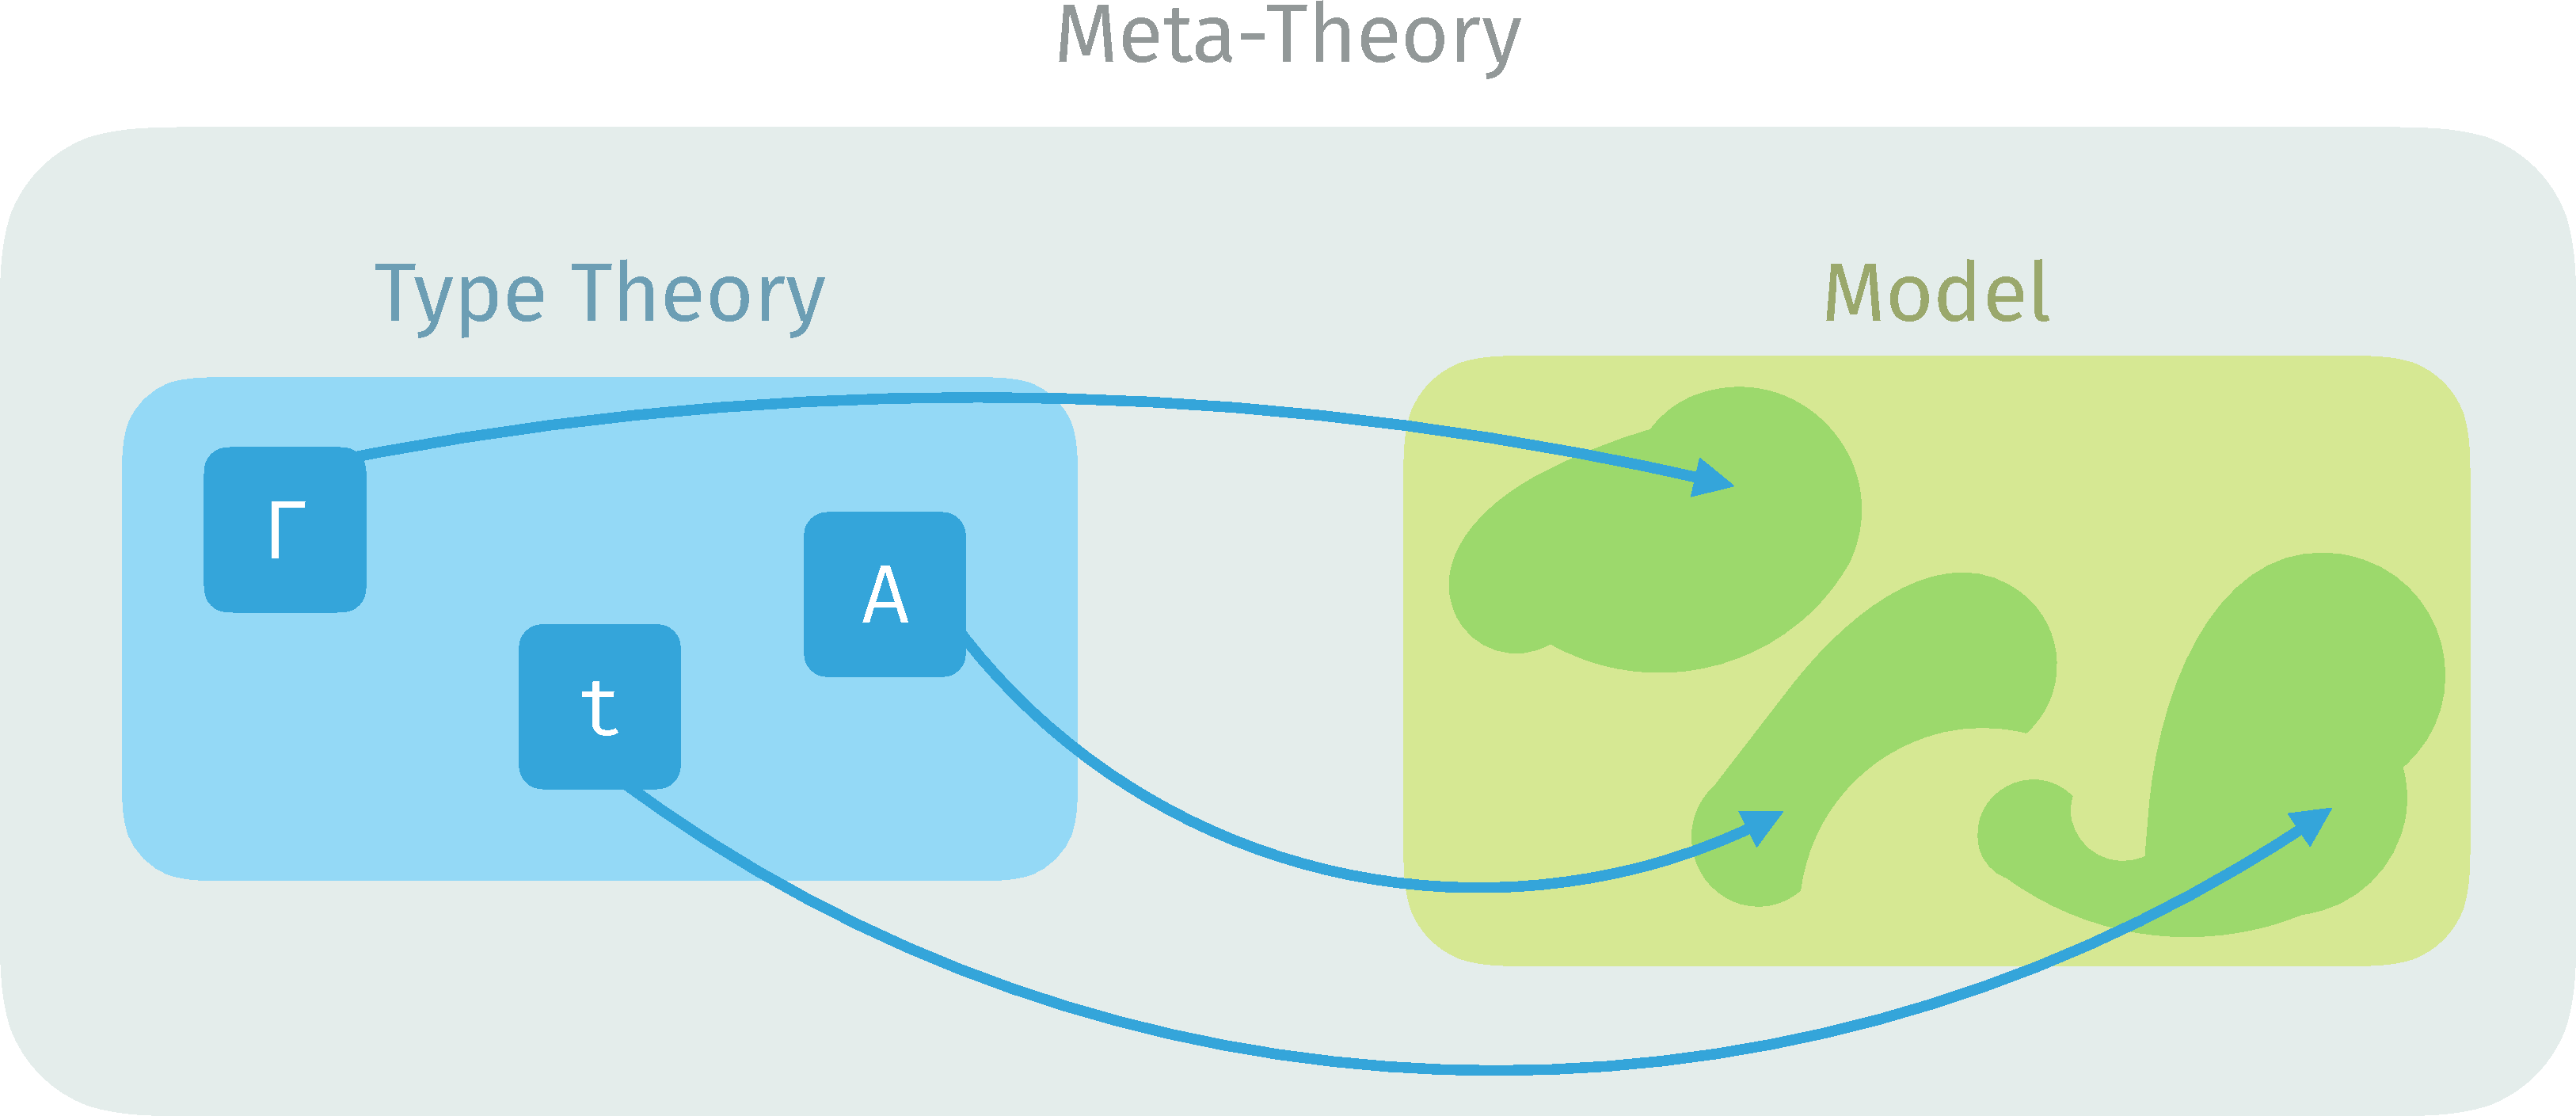
\includegraphics[width=0.9\textwidth]{model}
\end{figure}
To be more precise, a model is given by a class of objects to interpret
contexts, one for terms and one for types; but a model also provides an
interpretation to judgments in such a way that interpretation is coherent.
\todo{Make the definition clearer.}

\subsection{What can be proved using models}

\paragraph{Consistency.}

I already briefly mentioned this but the main point of models is to prove
consistency of a theory, relying on the already \emph{known} consistency of the
theory in which lives the model... At least in principle. It is however very
rare\sidenote{Impossible?} to \emph{know} that a theory is consistent, instead
we should see it as a theory we \emph{trust}, typically a theory that's widely
accepted as beeing consistent by the community of mathematicians.
This also applies to the meta-theory in which we show that the interpretation is
correct. As such it is best to keep it as simple as possible to avoid relying on
the consistency of too complicated objects.

\paragraph{Independence.}

Another interesing application of models is showing \emph{independence} of a
proposition.

\begin{definition}[Independent proposition]
  A proposition \(P\) is said to be independent from a theory \cT when neither
  \(P\) nor \(\neg P\) can be proven within \cT.
\end{definition}

A way to prove that some \(P\) is independent from \cT is to give a model of \cT
which validates \(P\) and another model which invalidates it (or validates
\(\neg P\)). Indeed if any one of \(P\) or \(\neg P\) %, let's say \(P\),
could be proven in \cT, then it would be valid in both models, leading to
at least one of them being inconsistent.

The fact that a proposition can neither be validated or invalidated in a theory
can come as surprising for some, especially in a classical mindset.
\reminder[-1.8cm]{Classical logic}{
  Classical logic is often characterised by the presence of the \acrshort{LEM}
  which consists in a proof of \(A \vee \neg A\).
}
Gödel's incompleteness theorems have to do with this.

\subsection{Gödel's incompleteness theorems}

\todo{Is it really the place? Should it even go in the proof theory chapter?}

\section{Set-theoretic models}

\section{Categorical models}

\section{Type-theoretic models}

\todo{translations, syntactical models, standard model}
% \setchapterpreamble[u]{\margintoc}
\chapter{Syntax and formalisation of type theory}
\labch{formalisation}

An interesting fact of type theory (and perhaps one its main selling points) is
that it is a suitable framework in which to reason about type theory.
That being said, representing type theory in itself isn't entirely
straightforward, and some care must be taken. There are actually several choices
to be made when representing type theory and they are not all equivalent or with
the same pros and cons.
I will detail some of them, spending more time on those I ended up choosing
and will try to motivate my choice.

\section{Representation of syntax}

I will first focus on the syntactical side of type theory.
The first important choice being how to represent variables.

\subsection{How to deal with variables}

When writing programs or expressions with binders on paper or on the computer
we will usually use \emph{names}, identifiers for variables like in
\(\lambda x. \lambda y. x\ y\), \(x\) refers to the variable bound by le
outermost \(\lambda\), while \(y\) referes to the variable bound by the
innermost.
The names aren't fundamental in what the term represents:
\(\lambda z. \lambda w. z\ w\) represents \emph{exactly} the same term.
We call this operation \(\alpha\)-renaming, here I \(\alpha\)-renamed \(x\)
to \(z\) and \(y\) to \(w\). This defines the notion of \(\alpha\)-equality
or \(\alpha\)-equivalence.
\[
  \lambda x. \lambda y. x\ y =_\alpha \lambda z. \lambda w. z\ w
\]
However variable names should only be thought of as an abstraction to represent
such terms and not a part of the syntax in itself.

Thinking in terms of variables name can lead to unpleasant examples where
\(\alpha\)-renaming might become a necessity.
For instance, \(\lambda x. \lambda x. x\) is perfectly valid but is easier to
read when renamed to \(\lambda y. \lambda x. x\). This process is called
\emph{shadowing}, when several variables bear the same name in scope, it is the
innermost that takes precedence. This principle is crucial for compositionality.

Even more problems arise when considering substitutions (after all, that is what
variables are for: to be substituted).
If you consider the term \(t \coloneqq x\ (\lambda x. x)\) we have two
occurrences of the name \(x\) but they do \emph{not} represent the same
variable, the first \(x\) is \emph{free} in the term, while the second is
\emph{bound} by the only \(\lambda\).
Now when substituting \(x\) for term \(u\) in \(t\), one has to be careful not
to replace the bound variable \(x\). The expected result is
\[
  t[x \sto u] = u\ (\lambda x. x)
\]
This used to be called \emph{capture-avoiding} substitutions, but I will call
them substitutions, because the operation yielding \(u\ (\lambda x. u)\)
is utterly rubbish and not deserving of a name.

Several solutions have been proposed to this ``problem'' like nominal
sets~\sidecite[-2.0cm]{pitts2001nominal},
\acrfull{HOAS}~\sidecite[-1.3cm]{pfenning1988higher} and de Bruijn indices or
levels~\sidecite[-1.0cm]{de1978lambda}.
In think de Bruijn indices are exactly what we want when dealing with
\(\lambda\)-terms as they carry the right amount of information.
The idea is to use natural numbers instead of names to indicate how many binders
to traverse before reaching the one introducing the variable.
\[
  \begin{array}{rcl}
    \lambda x.\ \lambda y.\ \lambda z.\ z
    &\to& \lambda\ \lambda\ \lambda\ \db{0} \\
    \lambda x.\ \lambda y.\ \lambda z.\ y
    &\to& \lambda\ \lambda\ \lambda\ \db{1} \\
    \lambda x.\ \lambda y.\ \lambda z.\ x
    &\to& \lambda\ \lambda\ \lambda\ \db{2}
  \end{array}
\]
In this setting the same variable can be represented in different ways:
\[
  \lambda x.\ x\ (\lambda y.\ x\ y)
\]
becomes
\[
  \lambda\ \db{0}\ (\lambda\ \db{1}\ \db{0})
\]
so that \(x\) is now written \(\db{0}\) and \(\db{1}\) depending on whether it
is referenced under the second \(\lambda\) or not.
The following diagram should make things more explicit.

\begin{center}
  \begin{tikzpicture}[remember picture]
    \node (term) {
      \(\subnode{la}{\(\lambda\)}\ \subnode{va}{\(\db{0}\)}\
      (\subnode{lb}{\(\lambda\)}\ \subnode{vb}{\(\db{1}\)}\
      \subnode{vc}{\(\db{0}\)})\)
    } ;
    \draw[barrow, bend right] (va.north) to (la.north) ;
    \draw[barrow, bend left] (vb.south) to (la.south) ;
    \draw[barrow, bend right] (vc.north) to (lb.north) ;
  \end{tikzpicture}
\end{center}

Using this representation, both \(\lambda x.x\) and \(\lambda y.y\) are written
\[
  \lambda\ \db{0}
\]
so that \(\alpha\)-equality is purely syntactic equality.
\(\alpha\)-renaming is not only a problem for pretty-printing.
This also solves the problem of substitutions potentially capturing free
variables: the term \(t \coloneqq x\ (\lambda x.\ x)\) of before is now
\(\db{n}\ (\lambda\ \db{0})\) where \(n\) is some number which should point to
somewhere in the context (same as the \(x\) it replaces).

Notice however that using de Bruijn indices, weakening---\ie putting a term into
an extended context---will now affect the term itself.
If you consider the following weakening, adding one variable \(z\) in the middle
of the context, doesn't affect the term using names.
\marginnote[1cm]{
  I use variables in the scope to make clear where the new variable is inserted
  in the nameless case.
}
\[
  x : A, y : B \vdash x\ y\ (\lambda u.\ x\ y\ u)
  \leadsto
  x : A, z : C, y : B \vdash x\ y\ (\lambda u.\ x\ y\ u)
\]
In the context of de Bruijn indices this becomes
\[
  A, B \vdash \db{1}\ \db{0}\ (\lambda\ \db{2}\ \db{1}\ \db{0})
  \leadsto
  A, C, B \vdash
  \highlight{\db{2}}\ \db{0}\ (\lambda\ \highlight{\db{3}}\ \db{1}\ \db{0})
\]


\subsection{Substitutions}

Another choice that is close to the representation of variable is that of
substitutions. There are several ways to represent a substitution in itself,
but I think the main question is whether to make them \emph{explicit} or not,
\ie part of the syntax or not.

\subsection{Annotations}
\todo{Curry vs Church for annotation of domain}
\todo{Annotation paranoia formal-type-theory (including typed or untyped equality?)}
\todo{Cardinal model}

\subsection{Universes and types}
\todo{Tarski/Russel universes}

\section{Representation of typing}

\todo{And conversion}
\todo{Well-typed syntax that I did not study in depth but needs to be
mentioned → maybe expose my idea that it isn't exactly the same,
notion of computation in the meta (→ translations)., HOAS?}
% \setchapterpreamble[u]{\margintoc}
\chapter{Translations}
\labch{translations}

Syntactical translations are a special case of program transformations suited
for type theory, and a method of choice to get models of type theories.
This is better studied in Simon Boulier's
thesis~\sidecite{boulier17:next-syntac-model-type-theor,boulier2018extending}
but in order to keep this document self contained, I will do my best to give a
meaningful excerpt here.

\section{Syntactical translations}

\subsection{Definition}
\labsubsec{syn-trans-def}

A \emph{syntactical} translation, as the name suggests, operates on the syntax
of terms. It has a source theory \cS and a target theory \cT with possibly
different syntax and typing rules---though usually \cS is an extension of \cT,
more on that later.

A translation is then given as two functions:
\begin{itemize}
  \item \([.]\) taking \cS terms to \cT terms;
  \item \(\transl{.}\) taking \cS types to \cT types.
\end{itemize}
And \(\transl{.}\) is---often---canonically extended to contexts:
\[
\begin{array}{lcl}
  \transl{\ctxempty} &\coloneqq& \ctxempty \\
  \transl{\Ga, x : A} &\coloneqq& \transl{\Ga}, x : \transl{A}
\end{array}
\]
\marginnote[-2cm]{
  It's not always the case that the \(\transl{\ctxempty}\) is also the empty
  context, and sometimes one variable is translated to several, but in a lot of
  cases it can still be encoded that way.
}

Usually, \(\transl{.}\) is built using \([.]\) and sometimes corresponds
exactly to \([.]\).
The translation is often done in an homomorphic way.

There are two main properties expected of a translation: type preservation
and preservation of falsehood.

\begin{definition}[Type preservation]
  A translation \([.], \transl{.}\) is type preserving when
  \(\isterm{\Ga}{t}{A}\) implies \(\isterm{\transl{\Ga}}{[t]}{\transl{A}}\).
\end{definition}

\begin{definition}[Preservation of falsehood]
  A translation \([.], \transl{.}\) from \cS to \cT is said to preserve
  falsehood when the translation of the empty type implies falsehood in the
  target:
  \[ \vdash_\cT \transl{\bot_\cS} \to \bot_\cT \]
\end{definition}

If a translation satisfies both those properties, we can conclude consistency
of \cS relatively to \cT.

\begin{theorem}[Relative consistency]
  If there is a translation from \cS to \cT that preserves typing and
  falsehood, then the consistency of \cT implies that of \cS.
\end{theorem}

\begin{proof}
  Assume a translation \([.], \transl{.}\) from \cS to \cT that preserves typing
  and falsehood. We'll prove the contraposition and assume inconsistency in
  \cS, that is the existence of a term \(t\) such that
  \[ \vdash_\cS t : \bot_\cS \]
  By preservation of typing, we get
  \[ \vdash_\cT [t] : \transl{\bot_\cS} \]
  Moreover, since the translation preserves falsehood, there is a term \(f\)
  such that \(\vdash_\cT f : \transl{\bot_\cS} \to \bot_\cT\).
  Thus, we conclude, using application that
  \[ \vdash_\cT f\ t : \bot_\cT \]
  in other words that \cT is also inconsistent.
\end{proof}

Relative consistency is all the more interesting when the source theory is more
complex than the target and even more so when \cT is theory that we trust.

Type preservation can be achieved by proving intermediary properties:
substitutivity, preservation of reduction and of conversion.

\begin{definition}[Substitutivity]
  A translation \([.], \transl{.}\) is substitutive when
  \[
    \begin{array}{lcl}
      [t\{x \sto u\}] &\coloneqq& [t]\{x \sto [u]\} \\
      \transl{A\{x \sto u\}} &\coloneqq& \transl{A}\{x \sto [u]\} \\
    \end{array}
  \]
\end{definition}

\begin{definition}[Preservation of reduction]
  A translation \([.], \transl{.}\) is said to preserve reduciton when
  \(u \red v\) implies \([u] \red [v]\) (and \(\transl{u} \red \transl{v}\)).
\end{definition}

\begin{definition}[Preservation of conversion]
  A translation \([.], \transl{.}\) is said to preserve reduciton when
  \(u \equiv v\) implies \([u] \equiv [v]\)
  (and \(\transl{u} \equiv \transl{v}\)).
\end{definition}

\subsection{Example: the \(\times\ \mathsf{bool}\) translation}

A simple yet non-trivial example of translation (or class of translations) is
the so-called \(\times\ \mathsf{bool}\) translation, again
from~\sidecite{boulier17:next-syntac-model-type-theor,boulier2018extending}.

As we said earlier, the source is going to be an extension of the target.
We'll keep the target pretty basic as a simple instance of \acrshort{ITT}
with a hierarchy of universes \(\Ty{i}\) (for \(i \in \mathbb{N}\)) with the
following rules:
\begin{itemize}
  \item \((\Ty{i}, \Ty{j}) \in \Ax\) for \(i \le j\);
  \item \((\Ty{i}, \Ty{j}, \Ty{k}) \in \Rl\) for \(i, j \le k\).
\end{itemize}
\marginnote[-1.6cm]{
  Refer to \frefsubsec{pts-itt} to see what theory we extend here.
}
Otherwise it has to feature a boolean type \(\bool\)---with the usual \(\ttrue\)
and \(\ffalse\)---product types \(A \times B\) as special
cases\sidenote{See \frefsec{inductive-types}.} of \(\Sigma\)-types,
and equality.
%
\begin{mathpar}
  \infer
    { }
    {\isterm{\Ga}{\bool}{\Ty{0}}}
  %

  \infer
    { }
    {\isterm{\Ga}{\ttrue}{\bool}}
  %

  \infer
    { }
    {\isterm{\Ga}{\ffalse}{\bool}}
  %
\end{mathpar}

The source is going to be the target extended with a new principle corresponding
to the negation of \acrlong{funext}, that is the existence of two functions
extensionaly equal, but not equal themselves.
%
\[
  \infer
    { }
    {
      \isterm
        {\Ga}
        {\notfunext}
        {\Sigma\ A\ B\ (f\ g : A \to B).\
          (\forall x.\ f\ x = g\ x) \times f \not= g
        }
    }
  %
\]
\marginnote[-1.4cm]{
  Inequality \(x \not= y\) is defined as the negation of equality, that is a map
  to the empty type: \(x = y \to \bot\).
}
%
We will write \(\Notfunext\) for the type of \(\notfunext\) in the following.

The idea is to inhabit this extra principle in the target which does not feature
it, or rather to inhabit its translation \(\transl{\Notfunext}\).
In order to differentiate functions of the target, while keeping them
observationally equal, we translate them by adding a boolean label to them.
Basically \(\lambda x. x\) is sent to \((\lambda x. x, \ttrue)\), the \(\ttrue\)
telling us the it might have come from the translation. Any function coming with
\(\ffalse\) instead will not be a translated term.

The translation is defined as follows:
%
\[
\begin{array}{lcl}
  [ x ] &\coloneqq& x \\ \relax
  [ \lambda (x : A).\ t ] &\coloneqq& (\lambda (x : \transl{A}).\ [t],\ttrue) \\
  \relax
  [ t\ u ] &\coloneqq& [t]\ [u] \\ \relax
  [ (u, v) ] &\coloneqq& ([u], [v]) \\ \relax
  [ p.1 ] &\coloneqq& [p].1 \\ \relax
  [ p.2 ] &\coloneqq& [p].2 \\ \relax
  [ \ttrue ] &\coloneqq& \ttrue \\ \relax
  [ \ffalse ] &\coloneqq& \ffalse \\ \relax
  [ \tif{t}{b. P}{u}{v} ] &\coloneqq& \tif{[t]}{b. \transl{P}}{[u]}{[v]} \\
  \relax
  [ \refl{A} u ] &\coloneqq& \refl{\transl{A}} [u] \\ \relax
  [ \J{A}{u}{x.e.P}{w}{v}{p} ] &\coloneqq&
  \J{\transl{A}}{[u]}{x.e.\transl{P}}{[w]}{[v]}{[p]} \\ \relax
  [ \Ty{i} ] &\coloneqq& \Ty{i} \\ \relax
  [ \Pi (x : A).\ B ] &\coloneqq&
  (\Pi (x : \transl{A}).\ \transl{B}) \times \bool \\ \relax
  [ \Sigma (x : A).\ B ] &\coloneqq& \Sigma (x:\transl{A}).\ \transl{B} \\
  \relax
  [ \bool ] &\coloneqq& \bool \\ \relax
  [ u =_A v ] &\coloneqq& [u] =_{\transl{A}} [v] \\ \relax
  \\
  \transl{A} &\coloneqq& [A]
\end{array}
\]
\marginnote[-0.6cm]{Notice how \(\transl{.}\) is just defined as \([.]\).}

I actually didn't provide the full translation here since I \emph{forgot}
the definition of \([\notfunext]\).
Writing down the term is rather tedious and boring, so instead I will give an
argument as to why it exists: you can provide any type for \(A\) and \(B\), for
instance \(\Ty{0}\) and then the for \(f\) and \(g\) we give
\((\lambda (x:\Ty{0}).\ x, \ttrue)\) and
\((\lambda (x:\Ty{0}).\ x, \ffalse)\) that will be pointwise equal (after
suffering the first projection) but different nonetheless.

This translation satisfies all the properties I mentioned in
\nrefsubsec{syn-trans-def}, including preservation of typing and of falsehood.
As such it shows that the negation of \acrshort{funext} is consistent in
\acrshort{ITT}. On the other hand, it can be shown that \acrshort{funext} is
also consistent, and as such independent from \acrshort{ITT}.
\reminder[-2.7cm]{Independence}{
  A proposition \(P\) is \emph{independent} from a theory \cT when both
  \(\cT + P\) and \(\cT + \neg P\) are consistent relatively to \cT.
}
For details, you should again refer to
\sidecite{boulier17:next-syntac-model-type-theor,boulier2018extending}
which gives a more comprehensive treatment of this and other translations.

\section{Other translations}

\todo{On derivations or intermediary representations}
\todo{Digression on notion of proof again?}

\section{Conversative extensions}

Translations are a nice way to obtain models of type theories, in particular
when showing that a certain principle extending a theory can be given an
interpretation and even computational content.
\marginnote[-1cm]{
  I did not dwell on this but as the new principle is given a definition in the
  target, we can \emph{pull out} its computational behaviour from there while
  respecting preservation of reduciton.
}

We can even be more restrictive on translations if we want to show that the new
principles are not adding new \emph{truths}, essentially saying that the
extension is more convenient while not really changing the logic.
There is an appropriate notion that is not specific to translations or even
type theory which is that of \emph{conservative extension}.

\begin{definition}[Conversative extension]
  An extension \(\cT_2\) of a theory \(\cT_1\) is \emph{conservative} if every
  theorem of \(\cT_2\) that can be stated in \(\cT_1\) is already a theorem of
  \(\cT_1\).
\end{definition}
\marginnote[-1.5cm]{
  An extension of a theory is a theory that proves at least as many theorems as
  the one it extends.
}
\todo{More on this in the proof theory chapter?}

In the context of type theories it can be reformulated as follows.

\begin{definition}[Conservative extension of a type theory]
  An extension \(\cT_2\) of a type theory \(\cT_1\) is \emph{conservative} if
  for every judgement \(\vdash_2 t : A\) such that \(\vdash_1 A\)
  (\ie \(A\) is a type in \(\cT_1\)), there exists \(t'\) such that
  \(\vdash_1 t' : A\).
\end{definition}
\todo{Define the notion of extension of type theory earlier?}

We will call a translation \emph{conservative} when it allows to exhibit that
the source theory \cS is a conservative extension of the target \cT, typically
when every type of \cT (\ie \(\vdash_\cT A\))---which makes sense in \cS since
it extends \cT---is sent to itself (\(\transl{A} = A\)) or at least implies
itself:
\[
  \vdash_\cT \transl{A} \to A
\]
This is kind of generalisation of preservation of falsehood.

The \(\times\ \bool\) translation is not conservative because
\[
  \vdash \transl{\Notfunext} \not\to \Notfunext
\]
and more generally \acrshort{ITT} extended with \(\Notfunext\) is not
conservative over \acrshort{ITT}.
I will present a conservative translation in \frefpart{elim-reflection}.

A simpler example could be that of encodings: say you want to add the \(\unit\)
type to a very basic theory with only \(\Pi\)-types.
\todo{Not clear it's a good example, it would require funext or SProp...}

\pagelayout{wide} % No margins
\addpart{Elimination of Reflection}
\labpart{elim-reflection}
\pagelayout{margin} % Restore margins

% \setchapterpreamble[u]{\margintoc}
\chapter{What I mean by elimination of reflection}
\labch{elim-reflection-intro}

We presented earlier \acrshort{ETT} and its defining reflection rule.
%
\reminder[-1.0cm]{Reflection rule}{
  \begin{equation*}
    \infer[]
      {\xisterm{\Ga}{e}{\Eq{A}{u}{v}}}
      {\xeqterm{\Ga}{u}{v}{A}}
    %
  \end{equation*}
  See \refdef{reflection}
}
%
The next few chapters are going to be dedicated to its elimination from type
theory: that is how to make a translation from \acrshort{ETT} to type theories
that do not feature reflection.

This work gave rise to a publication~\sidecite[0.2cm]{winterhalter:hal-01849166} that
focused on translating \acrshort{ETT} to \acrshort{ITT}.
However, with Simon Boulier we worked on another version translating directly to
\acrshort{WTT} which I'm going to present here.

\section{Nature of the translation}

\subsection{Syntactical translations are not possible}

First of all we have to wonder about what kind of translation is possible.
I presented in \nrefch{translations} the notion of syntactical translation.
Unfortunately it is not possible to devise a syntactical translation to
eliminate reflection from type theory.

Assume we have such a translation given by \(\transl{.}\) and \([.]\) such that
whenever \(\xisterm{\Gamma}{t}{A}\) we have
\(\isterm{\transl{\Gamma}}{[t]}{\transl{A}}\) in the target type theory.
Now let's say we have an inconsistent context in \acrshort{ETT}: \(\Gamma_\bot\)
(one can for instance assume \(0 = 1\) or \(\forall A, A\)), in such a context
anything can have any type because conversion has become trivial.
%
\marginnote[1.4cm]{
  Since \(\Gamma_\bot\) is inconsistent, anything can be proved from it,
  including the equality between the two types \(\mathbb{N}\) and \(\bot\).
  We then use reflection and conversion.
}
\begin{mathpar}
  \infer
    {
      \infer
        {\vdots}
        {\xisterm{\Gamma_\bot}{0}{\mathbb{N}}}
      \\
      \infer
        {
          \infer
            {\vdots}
            {\xisterm{\Gamma_\bot}{\_}{\mathbb{N} = \bot}}
          %
        }
        {\xeqterm{\Gamma_\bot}{\mathbb{N}}{\bot}{\Type}}
    }
    {\xisterm{\Gamma_\bot}{0}{\bot}}
  %
\end{mathpar}
%
It thus follows that in the target you have
\( \isterm{\transl{\Gamma_\bot}}{[0]}{\transl{\bot}} \).
Similarly you would have
\( \isterm{\transl{\Gamma_\bot}}{[0]}{\transl{\mathbb{N}}} \). This means
that both \(\bot\) and \(\mathbb{N}\) should be translated to similar things
(to convertible types in case the target theory has uniqueness of type), without
being able to exploit the knowledge that \(\Gamma_\bot\) is inconsistent
because of the syntactical nature of the translation.

\todo{Make things clearer}
Even worse, translations should preserve falsehood meaning in particular that
the translation of \(0\) should imply a proof of \(\bot\) in the target.
This is not a concrete proof that it is impossible but rather an argument
to see that such a translation would not behave well. One of the reasons is
that it would translate terms, types and contexts independently when it cannot.
Another is that an \acrshort{ETT} term does not contain any hints with respect
to the uses of reflection.

\subsection{Our translation(s)}

If we go back to the notion of proof, it becomes apparent that
syntactical translations do not work because we would not be translating proofs
but only partial ones; in other words terms in \acrshort{ETT} are not proofs
because they are insufficient to recover a typing derivation\sidenote{Because
type-checking is undecidable.}.
Thus comes the question of what is a \emph{suitable proof} in \acrshort{ETT}.
There is probably an intermediate structure between the term and the full
derivation that fits this role in the form of a term together with explicit
casts, however, in the setting of this thesis, we will still use complete
typing derivations in \acrshort{ETT} as \emph{proofs}.

Many problems stem from this approach unfortunately. Since we're translating
derivations there is no guarantee that the same term \(t\) in
\(\xisterm{\Gamma}{t}{A}\) and \(\xisterm{\Delta}{t}{B}\) will be translated
twice to the same term, this actually goes even for two different derivations
of the same judgement \(\xisterm{\Gamma}{t}{A}\).
This seems like a big obstacle to compositionality and would be iredeemable
without extra care regarding how individual judgements are translated.

We solve these problems by relating translations of a term (respectively
type and context) to the term itself, \emph{syntactically}.

\section{Target(s) of the translation}

Strictly speaking, elimination of reflection should be a translation from a
certain type theory \(T\) extended with reflection to \(T\) itself.
To fit this framework, we would provide a translation from \acrshort{ETT}
to \acrshort{ITT}. With Simon Boulier we discovered however that it is possible
to do something even stronger and go directly to a much weaker theory where
the notion of conversion is removed, \acrshort{WTT}.

\begin{figure}[hb]
  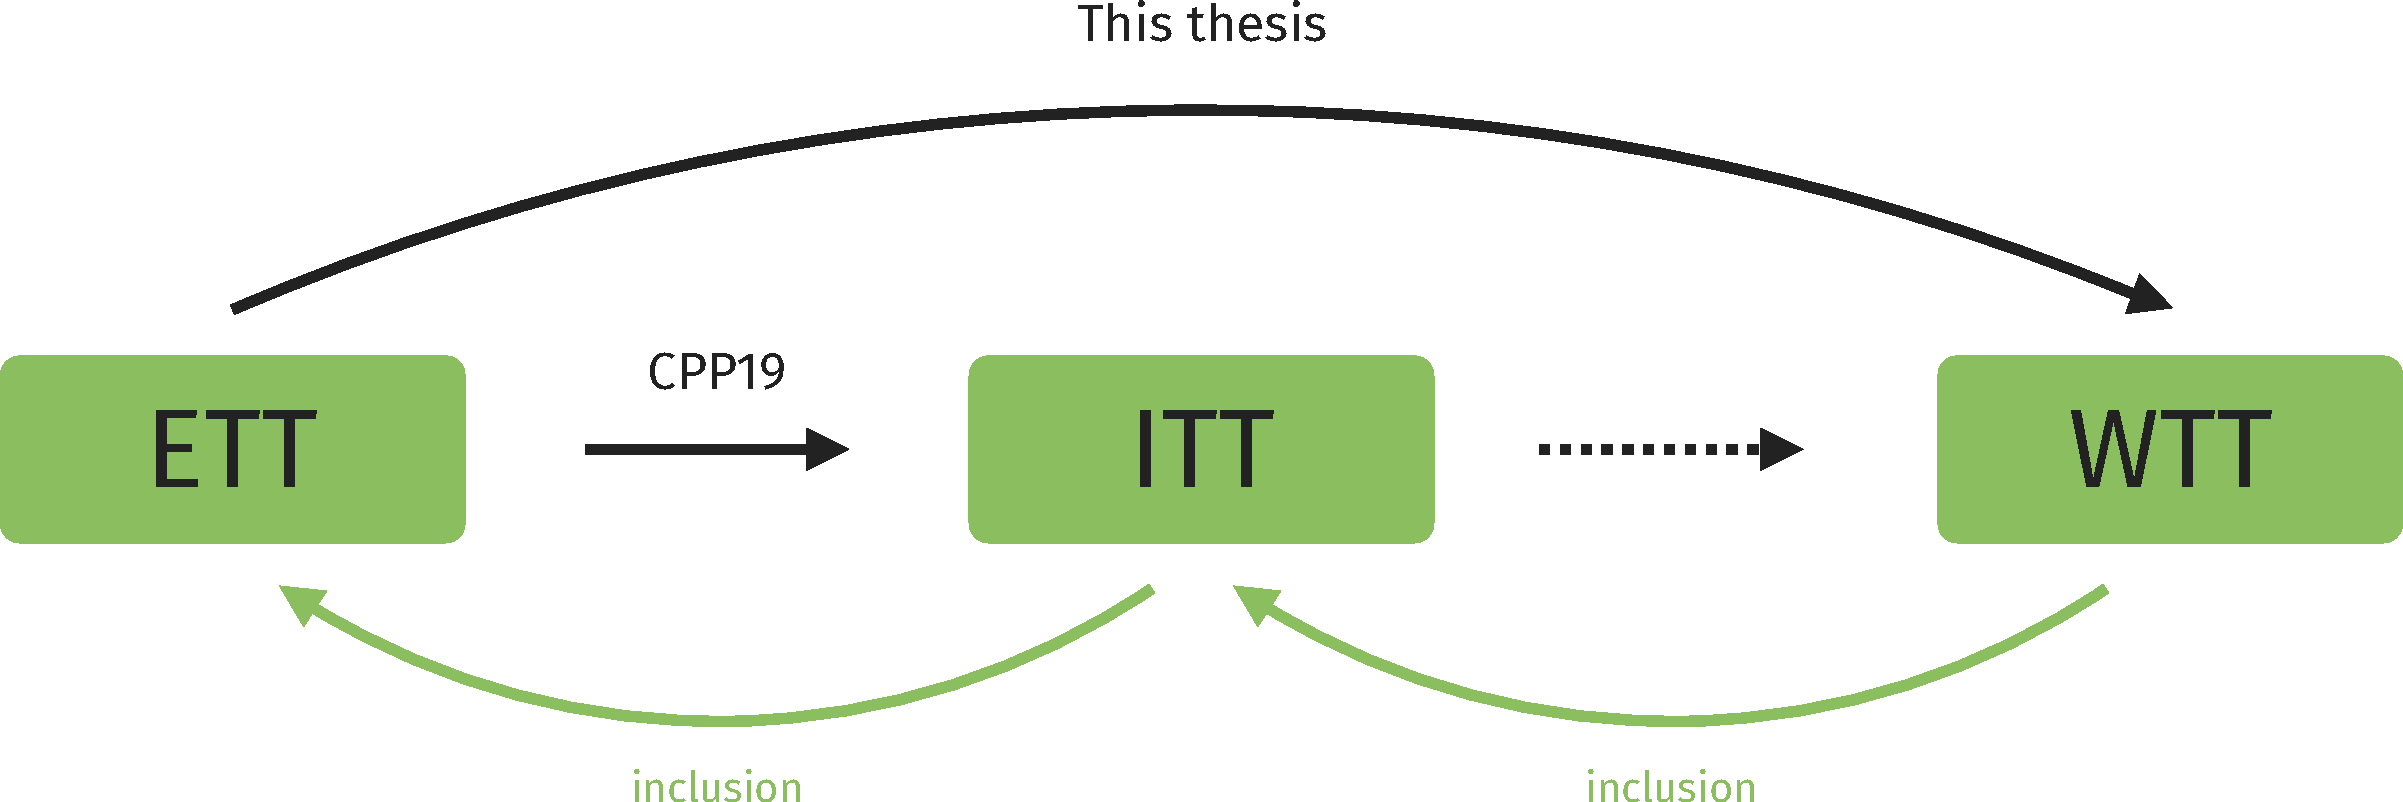
\includegraphics[width=0.9\textwidth]{elim-reflection-summary}
\end{figure}

From a translation of \acrshort{ETT} to \acrshort{WTT} we get an indirect one
from \acrshort{ETT} to \acrshort{ITT} as well as one from \acrshort{ITT} to
\acrshort{WTT}.
\marginnote[-0.5cm]{In both cases we exploit the fact that \acrshort{ETT}
extends \acrshort{ITT} which in turn extends \acrshort{WTT}.}

Note that in both cases, we're not dealing with arbitrary notions of
\acrshort{ITT} and \acrshort{WTT} but ones extended with some principles on
equality that will be described in \nrefsec{ext-principles}.
I will summarise the definitions for \acrshort{ETT}, \acrshort{ITT} and
\acrshort{WTT} I use for this translation in \nrefch{elim-reflection-framework}.

\section{Goal of the translation}

Why would we want to eliminate reflection? The first interest is that it
justfies that adding the reflection rule preserves consistency.
The main take-away however comes from the fact that we can show that
\acrshort{ETT} is conservative over both \acrshort{ITT} and \acrshort{WTT},
meaning that in order to prove a statement in one of those, it is enough
to prove it using the refleciton rule.
%
\reminder[-2.3cm]{Conservativity (roughly)}{
  A theory \cS is said to be \emph{conservative} over a
  theory \cT when every statement in \cT that
  is provable in \cS is also provable in \cT.
}
%

This can have practical use when proving theorems in a proof assistant like \Coq
which doesn't have reflection. If the translation is constructive, it gives
rise to an algorithm to transform a proof using reflection into a proof without.

The deduced \acrshort{ITT} to \acrshort{WTT} even teaches us that computation
is more of a commodity than a necessity as proofs can be transformed not to
exploit any computational behaviour.

\section{Extensionality principles on equality}
\labsec{ext-principles}

As we said earier, the \acrshort{ITT} and \acrshort{WTT} we consider are
actually extended with extensional principles on equality.
The main principles we require are \acrshort{UIP} and fonctional extensionality.
These two principles are valid statements of \acrshort{ITT} and \acrshort{WTT}
which are provable in \acrshort{ETT}, to show \acrshort{ETT} is a conservative
extension of the target, it must be provable in it; as it isn't the case we need
to extend the target with those principles.
\reminder[-3.6cm]{\acrshort{UIP}}{
\[ \Pi\ x \ y\ (e \ e' : x = y).\ e = e' \]
}
\reminder[-2.1cm]{\Acrshort{funext}}{
\[ \Pi\ f \ g .\ (\Pi x.\ f\ x = g\ x) \to f = g \]
}

For \acrshort{UIP} it can be show equivalent to Streicher's axiom K
\[
\begin{array}{rcl}
  \mathtt{K} & : & \Prod{A: s} \Prod{x :A} \Prod{e : x = x} e = \refl{x} \\
\end{array}
\]
where \(s\) is a sort, using the elimination on the identity type.
K is provable in \acrshort{ETT} by considering the type
\[
  \Prod{A: s} \Prod{x \ y:A} \Prod{e : x = y} e = \refl{x} \\
\]
which is well typed (using the reflection rule to show that $e$ has
type $x= x$) and which can be inhabited by elimination of the identity
type.

In the same way, \acrshort{funext} is provable in \acrshort{ETT} as shown by the
following diagram.
\[
\begin{array}{cll}
  &\Prod{x : A} f\ x = g\ x \\
  \to & x : A \vdash f\ x \equiv g\ x &
  \mbox{by reflection} \\
  \to &  (\lambda (x:A). {f \ x}) \equiv (\lambda{(x:A)}.{g \ x}) &
  \mbox{by congruence of $\equiv$} \\
  \to &  f \equiv g & \mbox{by $\eta$-law} \\
  \to &  f = g
\end{array}
\]

Therefore, applying our translation to the proofs of those theorems in
\acrshort{ETT} gives corresponding proofs of the same theorems in the target.

As I said, \acrshort{UIP} is independent from \acrshort{ITT}, as first shown by
Hofmann and Streicher using the groupoid model~\sidecite{groupoid-interp}, which
has recently been extended in the setting of univalent type theory using the
simplicial or cubical models~\sidecite{kapulkin2012simplicial,coquand:cubical}.

Similarly, \acrshort{funext} is independent from \acrshort{ITT}, it is folklore
but has recently been formalised by Boulier \emph{et al.} using a simple
syntactical translation~\sidecite{boulier17:next-syntac-model-type-theor}.

As previously said in \vrefsubsec{wtt}, \acrshort{WTT} has to be extended with
more principles in the vein of functional extensionality, like extensionality
of \(\Pi\)-types for similar reasons.

\section{Basic idea of the translation}

The basic idea behind the translation is to interpret conversion using the
internal notion of equality, \ie the identity type.
The naive approach would thus be to use transport to simulate the conversion
rule.
\reminder[-2.3cm]{Transport}{
Transport turns an equality \(e : A = B\) into a map
\(A \to B\).
}

This means however that for two terms \(a : A\) and \(b : B\) such that
\(A \equiv B\) and \(u \equiv v\) in \acrshort{ETT}, there translations
become comparable in the target only up-to the equality
between the two types. \([u] =_{[A]} [v]\) doesn't necessarilly make sense
anymore.

To solve this proper we use instead a notion of heterogeneous equality.
This is also the approach followed by
Oury~\sidecite[1.7cm]{oury2005extensionality}
although we decided on a slightly different presentations of heterogeneous
equality to avoid the axioms involved with the use of \acrshort{JMeq}.
\reminder[-2.3cm]{Heterogenous equality}{
\(\Heq{T}{t}{U}{u}\), equality between \(t : T\) and \(u : U\) is defined as
\(\Sum{p:\Eq{}{T}{U}} \Eq{}{\transpo{p}\ t}{u}\).
}

During the translation, the same term occurring twice can be
translated in two different manners, if the corresponding typing
derivations are different. Even the types of the two different
translations may be different.
%
However, we have the strong property that any two translations of the
same term only differ in places where transports of proofs of equality have been
injected.

To keep track of this property, we introduce the relation $t \sim t'$
between two terms of the target, of possibly different
types\sidenote{The relation is fully syntactic.}.
%
The crux of the proof of the translation is to guarantee that for
every two terms $t_1$ and $t_2$ such that $\isterm{\Ga}{t_1}{T_1}$,
$\isterm{\Ga}{t_2}{T_2}$ and $t_1 \sim t_2$, there exists $p$ such that
$\isterm{\Ga} {p} {\Heq{{T_1}} {{t_1}} {{T_2}} {{t_2}}}$.

During the proof, variables of different but (propositionally) equal
types are introduced and the context cannot be maintained to be the same
for both $t_1$ and $t_2$. Therefore, the translation needs to keep
track of this duplication of variables, plus a proof that they are
heterogeneously equal.
%
This mechanism is similar to what happens in the (relational) internal
parametricity translation in \acrshort{ITT} introduced by
\sidecite[-0.4cm]{bernardy2012proofs} and recently rephrased in the setting of
\MetaCoq~\sidecite{DBLP:conf/itp/AnandBCST18}. Namely, a context is not
translated as a telescope of variables, but as a telescope of triples
consisting of two variables plus a witness that they are in the
parametric relation: \(x : A\) is (roughly) sent to
\(x_1 : A_1, x_2 : A_2, x_\varepsilon : A_\varepsilon\ x_1\ x_2\).
%
In our setting, this amounts to consider telescope of triples
consisting of two variables plus a witness that they are
heterogeneously equal. We can express this by considering the
following dependent sums:
\[
\Pack{A_1}{A_2} := \Sum{x:A_1} \Sum{y:A_2} \Heq{A_1}{x}{A_2}{y}.
\]

This presentation inspired by the parametricity translation is crucial
in order to get an effective translation, because it is necessary to
keep track of the evolution of contexts when doing the translation on
open terms.
%
This ingredient is missing in Oury's work~\sidecite{oury2005extensionality},
which prevents him from deducing an effective (\ie constructive and
computable) translation from his theorem.
The construction of this relation is discussed in \nrefch{elim-rel}.
% \setchapterpreamble[u]{\margintoc}
\chapter{Framework}
\labch{elim-reflection-framework}

Now that the problem is stated, I will clearly define what the type theories
I will use as source and target. This is a bit redundant with \nrefch{flavours}
but I think it's worthwhile to make it clear what the translation is operating
on.

\section{Syntax(es)}

To make things simple I will consider the syntax of \acrshort{ITT} and
\acrshort{WTT} as extensions of the syntax of \acrshort{ETT}.
Actually, \acrshort{WTT} will also extend \acrshort{ITT}.

\subsection{Syntax of \acrshort{ETT}}

First, comes the syntax of \acrshort{ETT}.

\[
  \begin{array}{l@{~\,}r@{~\,}l}
    s &\in& \cS \\
    T,A,B,t,u,v &\bnf& x \bnfor \lam{x:A}{B} t \bnfor \app{t}{x:A}{B}{u} \\
    &\bnfor& \pair{x:A}{B}{u}{v} \bnfor \pio{x:A}{B}{p} \bnfor \pit{x:A}{B}{p} \\
    &\bnfor& \refl{A} u \bnfor \J{A}{u}{x.e.P}{w}{v}{p} \\
    % &\bnfor& \funext{x:A}{B}{f}{g}{e} \bnfor \uip{A}{u}{v}{p}{q} \\
    &\bnfor& \ax{n} \\
    &\bnfor& s \bnfor \Prod{x:A} B \bnfor \Sum{x:A} B \bnfor \Eq{A}{u}{v} \\
    \Ga, \D &\bnf& \ctxempty \bnfor \Ga, x:A \\
    \Sigma &\bnf& \ctxempty \bnfor \Sigma, n:A
  \end{array}
\]

\paragraph{Sorts.}

Sorts are kept abstract (as represented by the generic \cS) but are not
unrestricted. With the sorts should come the sort of a sort (or successor
sort) \(\succs{s}\), the sort of a \(\Pi\)-type \(\pisort{s_1}{s_2}\)
where \(s_1\) and \(s_2\) are the sorts of the domain and codomain respecitvely,
and likewise for each constructor.
These are functions, so the underlying \acrshort{PTS} is functional.
\todo{Define fun PTS}
Additionally, we ask that equality of sorts is decidable and that the successor
function is injective:
\[
  \succs{s_1} = \succs{s_2} \longrightarrow s_1 = s_2.
\]
Keeping the sorts abstract means that the proof can be instantiated with a lot
of different hierarchies, as long as they do not feature cumulativity
unfortunately. This will help us apply our result in the homotopy framework.

\paragraph{Annotations.}

Although it may look like a technical detail, the use of annotation is more
fundamental in \acrshort{ETT} than it is in \acrshort{ITT}/\acrshort{WTT}
where it is irrelevant and doesn't affect the theory.
This is actually one of the main differences between our work
(and that of Martin Hofmann~\sidecite{hofmann1995conservativity} who has a
similar presentation) and the work of Nicolas
Oury~\sidecite[0.7cm]{oury2005extensionality}.

Indeed, by using the standard model where types are interpreted as
cardinals rather than sets, it is possible to see that the equality
$\nat \to \nat = \nat \to \bool$ is independent from the theory, it is
thus possible to assume it (as an axiom, or for those that would still
not be convinced, simply under a $\lambda$ that would introduce this
equality).  In that context, the identity map $\lambda(x : \nat).\ x$
can be given the type $\nat \to \bool$ and we thus type
$(\lambda(x : \nat).\ x)\ \zero : \bool$.  Moreover, the
$\beta$-reduction of the non-annotated system used by Oury concludes
that this expression reduces to $\zero$, but cannot be given the type
$\bool$ (as we said, the equality $\nat \to \nat = \nat \to \bool$ is
independent from the theory, so the context is consistent). This means
we lack subject reduction in this case (or unique typing,
depending on how we see the issue).  Our presentation has a blocked
$\beta$-reduction limited to matching annotations:
$\app{(\lam{x:A}{B}\ t)}{x:A}{B}{u} = t[x \sto u]$, from which subject
reduction and unique typing follow.

\marginnote{
  \[
    \infer[JMAPP]
      {
        \Heq{\forall (x : U_1). V_1}{f_1}{\forall (x : U_2). V_2}{f_2} \\
        \Heq{U_1}{u_1}{U_2}{u_2}
      }
      {\Heq{V_1[x \sto u_1]}{f_1\ u_1}{V_2[x \sto u_2]}{f_2\ u_2}}
    %
  \]
}
Although subtle, this difference is responsible for Oury's need for an
extra axiom. Indeed, to treat the case of equality of applications in
his proof, he needs to assume the congruence rule for heterogeneous
equality of applications, which is not provable when formulated with
\acrshort{JMeq}. Thanks to annotations and our notion of heterogeneous equality,
we can prove this congruence rule for applications.
\todo{Maybe move this earlier? At least part of this discussion should already
be treated.}

\paragraph{Axioms.}

\subsection{Syntax of \acrshort{ITT}}

\subsection{Syntax of \acrshort{WTT}}

\subsection{Isn't \acrshort{ETT} no longer an extension of either \acrshort{ITT}
or \acrshort{WTT}?}

\todo{Maybe separate ITT and WTT as syntactical extensions, then talk
about how ETT is no longer an extension but it doesn't really matter
conservativity can still be stated with a simple translation from ITT/WTT to
ETT.}
\todo{WTT is not included right now}

\section{Typing rules}
\todo{Mention no cumulativity}
% \setchapterpreamble[u]{\margintoc}
\chapter{Relating translated expressions}
\labch{elim-rel}

We want to define a relation on terms that equates two terms that are
the same up to transport.
%
This begs the question of what notion of transport is going to be
used.
%
Transport can be defined from elimination of equality as in \nrefch{usual-defs}.
However, in order not to confuse the transports added by the
translation with the transports that were already present in the
source, we consider $\transpo{p}$ as part of the syntax in the
reasoning. It will be unfolded to its definition only after the
complete translation is performed.
%
This idea is not novel as Hofmann already had a $\mathsf{Subst}$ operator that
was part of his \acrshort{ITT} (noted TT\textsubscript{I} in his
paper~\sidecite{hofmann1995conservativity}).

\section{Relating terms and their translation}

We first define the (purely syntactic) relation $\ir$ between \acrshort{ETT}
terms and target terms by saying the translated term must be a decoration of the
first term by transports.
Its purpose is to state how close to the original term its translation is.
% In the definition, the most important rule is highlighted.

\marginnote[1cm]{
  As you can see, this relation doesn't talk about \acrshort{ITT} or
  \acrshort{WTT} specific terms.
}
\begin{mathpar}

  \highlight{
    \infer[]
      {t_1 \ir t_2}
      {t_1 \ir \transpo{p}\ t_2}
    %
  }

  \infer[]
    { }
    {x \ir x}
  %

  \infer[]
    {A_1 \ir A_2 \\
     B_1 \ir B_2
    }
    {\Prod{x:A_1} B_1 \ir \Prod{x:A_2} B_2}
  %

  \infer[]
    {A_1 \ir A_2 \\
     B_1 \ir B_2
    }
    {\Sum{x:A_1} B_1 \ir \Sum{x:A_2} B_2}
  %

  \infer[]
    {A_1 \ir A_2 \\
     u_1 \ir u_2 \\
     v_1 \ir v_2
    }
    {\Eq{A_1}{u_1}{v_1} \ir \Eq{A_2}{u_2}{v_2}}
  %

  \infer[]
    { }
    {s \ir s}
  %

  \infer[]
    {A_1 \ir A_2 \\
     B_1 \ir B_2 \\
     t_1 \ir t_2
    }
    {\lam{x:A_1}{B_1} t_1 \ir \lam{x:A_2}{B_2} t_2}
  %

  \infer[]
    {t_1 \ir t_2 \\
     A_1 \ir A_2 \\
     B_1 \ir B_2 \\
     u_1 \ir u_2
    }
    {\app{t_1}{x:A_1}{B_1}{u_1} \ir \app{t_2}{x:A_2}{B_2}{u_2}}
  %

  \infer[]
    {A_1 \ir A_2 \\
     B_1 \ir B_2 \\
     t_1 \ir t_2 \\
     u_1 \ir u_2
    }
    {\pair{x:A_1}{B_1}{t_1}{u_1} \ir \pair{x:A_2}{B_2}{t_2}{u_2}}
  %

  \infer[]
    {A_1 \ir A_2 \\
     B_1 \ir B_2 \\
     p_1 \ir p_2
    }
    {\pio{x:A_1}{B_1}{p_1} \ir \pio{x:A_2}{B_1}{p_2}}
  %

  \infer[]
    {A_1 \ir A_2 \\
     B_1 \ir B_2 \\
     p_1 \ir p_2
    }
    {\pit{x:A_1}{B_1}{p_1} \ir \pit{x:A_2}{B_2}{p_2}}
  %

  \infer[]
    {A_1 \ir A_2 \\
     u_1 \ir u_2
    }
    {\refl{A_1} u_1 \ir \refl{A_2} u_2}
  %

  \infer
    {
      A_1 \ir A_2 \\
      u_1 \ir u_2 \\
      P_1 \ir P_2 \\
      w_1 \ir w_2 \\
      v_1 \ir v_2 \\
      p_1 \ir p_2
    }
    {
      \J{A_1}{u_1}{x.e.P_1}{w_1}{v_1}{p_1} \ir
      \J{A_2}{u_2}{x.e.P_2}{w_2}{v_2}{p_2}
    }
  %
\end{mathpar}

From this relation we build a new one (\(\sim\)) between translated terms.
\(u \sim v\) basically means that \(u\) and \(v\) are both decorations of the
same term.

\[
  \sim\ \coloneqq\ \sqsupset^+ . \ir^+
\]

In order to better reason about it however, we actually define it inductively
again.

\begin{mathpar}
  \highlight{
    \infer[]
      {t_1 \sim t_2}
      {\transpo{p}\ t_1 \sim t_2}
    %
  }

  \highlight{
    \infer[]
      {t_1 \sim t_2}
      {t_1 \sim \transpo{p}\ t_2}
    %
  }

  \infer[]
    {A_1 \sim A_2 \\
     B_1 \sim B_2
    }
    {\Prod{x:A_1} B_1 \sim \Prod{x:A_2} B_2}
  %

  \infer[]
    {A_1 \sim A_2 \\
     B_1 \sim B_2
    }
    {\Sum{x:A_1} B_1 \sim \Sum{x:A_2} B_2}
  %

  \infer[]
    {A_1 \sim A_2 \\
     u_1 \sim u_2 \\
     v_1 \sim v_2
    }
    {\Eq{A_1}{u_1}{v_1} \sim \Eq{A_2}{u_2}{v_2}}
  %

  \infer[]
    { }
    {s \sim s}
  %

  \infer[]
    {A_1 \sim A_2 \\
     B_1 \sim B_2 \\
     t_1 \sim t_2
    }
    {\lam{x:A_1}{B_1} t_1 \sim \lam{x:A_2}{B_2} t_2}
  %

  \infer[]
    {t_1 \sim t_2 \\
     A_1 \sim A_2 \\
     B_1 \sim B_2 \\
     u_1 \sim u_2
    }
    {\app{t_1}{x:A_1}{B_1}{u_1} \sim \app{t_2}{x:A_2}{B_2}{u_2}}
  %

  \infer[]
    {A_1 \sim A_2 \\
     B_1 \sim B_2 \\
     t_1 \sim t_2 \\
     u_1 \sim u_2
    }
    {\pair{x:A_1}{B_1}{t_1}{u_1} \sim \pair{x:A_2}{B_2}{t_2}{u_2}}
  %

  \infer[]
    {A_1 \sim A_2 \\
     B_1 \sim B_2 \\
     p_1 \sim p_2
    }
    {\pio{x:A_1}{B_1}{p_1} \sim \pio{x:A_2}{B_1}{p_2}}
  %

  \infer[]
    {A_1 \sim A_2 \\
     B_1 \sim B_2 \\
     p_1 \sim p_2
    }
    {\pit{x:A_1}{B_1}{p_1} \sim \pit{x:A_2}{B_2}{p_2}}
  %

  \infer[]
    {A_1 \sim A_2 \\
     u_1 \sim u_2
    }
    {\refl{A_1} u_1 \sim \refl{A_2} u_2}
  %

  \infer
    {
      A_1 \sim A_2 \\
      u_1 \sim u_2 \\
      P_1 \sim P_2 \\
      w_1 \sim w_2 \\
      v_1 \sim v_2 \\
      p_1 \sim p_2
    }
    {
      \J{A_1}{u_1}{x.e.P_1}{w_1}{v_1}{p_1} \sim
      \J{A_2}{u_2}{x.e.P_2}{w_2}{v_2}{p_2}
    }
  %
\end{mathpar}

Once more, constructions specific to \acrshort{ITT} or \acrshort{WTT} are not
related with \(\sim\): these will only appear in the equalities that are
transported (the \(p\) in the highlighted rules).

\section{Properties of the relation}

As I just remarked, the relation is not reflexive; but only in that respect
doest it fall short of being an equivalence relation.

\begin{lemma}[$\sim$ is a partial equivalence relation]
  \lablemma{sim-er}
  $\sim$ is symmetric and transitive.
\end{lemma}

% \begin{proof}
%   For reflexivity we proceed by induction on the term.
% \end{proof}

The goal is to prove that two terms in this relation, that are well-typed in the
target type theory, are heterogeneously equal.

\todo{Properties on heterogeneous equality should have their own section.
Maybe with its def in usual defs, and a reminder here.}
Heterogeneous equality is reflexive, symmetric and transitive.
Thanks to \acrshort{UIP}, heterogeneous equality collapses to regular equality
when taken on the same type on both sides.

\begin{lemma}
  \lablemma{uip-cong}
  If $\isterm{\Ga}{e}{\Heq{A}{u}{A}{v}}$
  then there exists $p$ such that $\isterm{\Ga}{p}{\Eq{A}{u}{v}}$.
\end{lemma}

\begin{proof}
  This holds thanks to \acrshort{UIP} on equality, which implies K, and so the
  proof of $A = A$ can be taken to be reflexivity.
\end{proof}

\begin{remark}
  As a corollary, $\Heqs$ on types corresponds to equality.
  Indeed when we have $\isterm{\Ga}{e}{\Heq{s}{A}{s'}{B}}$ we have
  that $\Eq{}{s}{s'}$, which implies that $s$ and $s'$ have the same sort
  and thus are syntactically the same (by an inversion argument).
\end{remark}

Before we can prove the fundamental lemma stating that two terms in relation
are heterogeneously equal, we need to consider another construction.
%
As explained earlier~\misref, when proving the property by induction on terms, we
introduce variables in the context that are equal only up to heterogeneous
equality.
%
This phenomenon is similar to what happens in the parametricity
translation~\sidecite{bernardy2012proofs}.
%
Our fundamental lemma on the decoration relation $\sim$ assumes two
related terms of potentially different types $T1$ and $T2$ to produce an
heterogeneous equality between them. For induction to go through under
binders (e.g. for dependent products and abstractions), we hence need to
consider the two terms under different, but heterogeneously equal
contexts.
%
Therefore, the context we produce will not only be a telescope of
variables, but rather a telescope of triples consisting of two variables
of possibly different types, and a witness that they are heterogeneously
equal.
%
To make this precise, we define the following macro:
%
\[
\Pack{A_1}{A_2} := \Sum{x:A_1} \Sum{y:A_2} \Heq{}{x}{}{y}
\]
together with its projections
\begin{mathpar}
  \ProjO{p} := \pio{}{}{p}

  \ProjT{p} := \pio{}{}{\pit{}{}{p}}

  \ProjE{p} := \pit{}{}{\pit{}{}{p}}.
\end{mathpar}
%
We can then extend this notion canonically to contexts of the same
length that are well formed using the same sorts:
\marginnote[-0,5cm]{
  That is \(\Ga_1 \coloneqq x_1 : A_1, \dots, x_n : A_n\),
  \(\Ga_2 \coloneqq y_1 : B_1, \dots, y_n : B_n\) where
  there exists \(s_i\) such that \(A_i : s_i\) and \(B_i : s_i\) for each \(i\).
}
%
\[
\begin{array}{l}
    \Pack{(\Ga_1, x:A_1)}{(\Ga_2, x:A_2)} := \\
    (\Pack{\Ga_1}{\Ga_2}),
    x : \Pack{(\llift{\gamma}{}{A_1})}{(\rlift{\gamma}{}{A_2})} \\
    \\
    \Pack{\ctxempty}{\ctxempty} := \ctxempty.
\end{array}
\]
%
When we pack contexts, we also need to apply the correct projections for
the types in that context to still make sense. Assuming two contexts
$\Ga_1$ and $\Ga_2$ of the same length, we can define left and right
substitutions:
\[
\begin{array}{ll}
  \gamma_1 &:= [ x \leftarrow \ProjO{x}\ |\ (x : \_) \in \Ga_1 ] \\
  \gamma_2 &:= [ x \leftarrow \ProjT{x}\ |\ (x : \_) \in \Ga_2 ].
\end{array}
\]
These substitutions implement lifting of terms to packed contexts:
we have
$\isterm{\Ga, \Pack{\Ga_1}{\Ga_2}}{\llift{\gamma}{}{t}}{\llift{\gamma}{}{A}}$
whenever $\isterm{\Ga, \Ga_1}{t}{A}$
and
$\isterm{\Ga, \Pack{\Ga_1}{\Ga_2}}{\rlift{\gamma}{}{t}}{\rlift{\gamma}{}{A}}$
whenever $\isterm{\Ga, \Ga_2}{t}{A}$.

For readability, when $\Ga_1$ and $\Ga_2$ are understood we will write $\Gp$ for
$\Pack{\Ga_1}{\Ga_2}$.

Implicitly, whenever we use the notation $\Pack{\Ga_1}{\Ga_2}$ it means that
the two contexts are of the same length and well-formed with the same
sorts.
%
We can now tackle the fundamental lemma.

\begin{lemma}[Fundamental lemma]
  \lablemma{sim-cong}
  Let $t_1$ and $t_2$ be two terms such that \(t_1 \sim t_2\).
  For all contexts \(\Ga\), \(\Ga_1\) and \(\Ga_2\) we can \emph{construct}
  another term \(p\) such that whenever $\isterm{\Ga, \Ga_1}{t_1}{T_1}$ and
  $\isterm{\Ga, \Ga_2}{t_2}{T_2}$ we have
  $\isterm{\Ga, \Pack{\Ga_1}{\Ga_2}}
          {p}
          {\Heq{\llift{\gamma}{}{T_1}}
               {\llift{\gamma}{}{t_1}}
               {\rlift{\gamma}{}{T_2}}
               {\rlift{\gamma}{}{t_2}}}$.
\end{lemma}

\begin{proof}
  The proof is by induction on the derivation of $t_1 \sim t_2$. We show
  the three most interesting cases:

  \begin{itemize}
  \item \textsc{Var}
    \[
      \infer[]
        { }
        {x \sim x}
      %
    \]
    If $x$ belongs to $\Ga$, we apply reflexivity---together with uniqueness of
    typing~\eqref{lemma:uniq}---to conclude.
    Otherwise, $\ProjE{x}$ has the expected type (since
    $\llift{\gamma}{}{x} \equiv \ProjO{x}$ and $\rlift{\gamma}{}{x} \equiv \ProjT{x}$).

  \item \textsc{Application}
    \[
      \infer[]
        {t_1 \sim t_2 \\
         A_1 \sim A_2 \\
         B_1 \sim B_2 \\
         u_1 \sim u_2
        }
        {\app{t_1}{x:A_1}{B_1}{u_1} \sim \app{t_2}{x:A_2}{B_2}{u_2}}
      %
    \]
    We have $\isterm{\Ga, \Ga_1}{\app{t_1}{x:A_1}{B_1}{u_1}}{T_1}$ and
    $\isterm{\Ga, \Ga_2}{\app{t_2}{x:A_2}{B_2}{u_2}}{T_2}$ which means by
    inversion~\eqref{lemma:inversion} that the subterms are well-typed.
    We apply the induction hypothesis and then conclude.
  \item \textsc{TransportLeft}
    \[
      \infer[]
        {t_1 \sim t_2}
        {\transpo{p}\ t_1 \sim t_2}
      %
    \]
    We have $\isterm{\Ga, \Ga_1}{\transpo{p}\ t_1}{T_1}$ and
    $\isterm{\Ga, \Ga_2}{t_2}{T_2}$.
    By inversion~\eqref{lemma:inversion} we have
    $\isterm{\Ga, \Ga_1}{p}{\Eq{}{T_1'}{T_1}}$ and
    $\isterm{\Ga, \Ga_1}{t_1}{T_1'}$.
    By induction hypothesis we have $e$ such that
    $\isterm{\Ga, \Gp}{e}{\Heq{}{\llift{\gamma}{}{t_1}}{}{\rlift{\gamma}{}{t_2}}}$.
    From transitivity and symmetry we only need to provide a proof of
    $\Heq{}{\llift{\gamma}{}{t_1}}{}{\transpo{\llift{\gamma}{}{p}}\ \llift{\gamma}{}{t_1}}$ which is inhabited by
    $\pair{\_}{\_}{\llift{\gamma}{}{p}}{\refl{} (\transpo{\llift{\gamma}{}{p}}\ \llift{\gamma}{}{t_1})}$.
  \end{itemize}

  The complete proof can be found in \frefsec{proof-fund-lemma}.
  \todo{Should I keep it though?}
\end{proof}

We can also prove that $\sim$ preserves substitution.

\begin{lemma}
  If $t_1 \sim t_2$ and $u_1 \sim u_2$ then
  $t_1[x \sto u_1] \sim t_2[x \sto u_2]$.
\end{lemma}

\begin{proof}
  We proceed by induction on the derivation of $t_1 \sim t_2$.
\end{proof}

The fundamental lemma, as the name suggests, is the main ingredient to proving
the translation correct (and actually building the translation). Now that we
have it, we can proceed with the translation.
% \setchapterpreamble[u]{\margintoc}
\chapter{Translation from \acrshort{ETT} to \acrshort{ITT} and \acrshort{WTT}}
\labch{elim-trans}

\section{The Translation}
\labsec{the-translation}

We now define the translations (let us stress the plural here) of an
extensional judgment. We extend $\ir$ canonically to contexts
($\Ga \ir \Gb$ when they bind the same variables and the types are in
relation for $\ir$).

Before defining the translation, we define a set
$\transl{\xisterm{\Ga}{t}{A}}$ of typing judgments
in ITT associated to a typing judgment $\xisterm{\Ga}{t}{A}$ in ETT.
%
The idea is that this set describes all the possible translations that
lead to the expected property. When
$\isterm{\Gb}{\tb}{\Ab} \in \transl{\xisterm{\Ga}{t}{A}}$, we say that
$\isterm{\Gb}{\tb}{\Ab}$ realises $\xisterm{\Ga}{t}{A}$. The
translation will be given by showing that this set is inhabited by
induction on the derivation.

\begin{definition}[Characterisation of possible translations]
  \leavevmode
  \begin{itemize}
    \item For any $\xisctx{\Ga}$ we define $\transl{\xisctx{\Ga}}$ as a set of
    valid judgments (in ITT) such that
    $\isctx{\Gb} \in \transl{\xisctx{\Ga}}$ if and only if $\Ga \ir \Gb$.

    \item Similarly, $\isterm{\Gb}{\tb}{\Ab} \in \transl{\xisterm{\Ga}{t}{A}}$
    iff $\isctx{\Gb} \in \transl{\xisctx{\Ga}}$ and $A \ir \Ab$ and $t \ir \tb$.
  \end{itemize}
\end{definition}

In order to better master the shape of the produced realiser, we state the
following lemma which shows that it has the same head
type constructor as the type it realises.
%
This is important for instance for the case of an application, where we
do not know a priori if the translated function has a dependent product
type, which is required to be able to use the typing rule for application.

\begin{lemma}
  \lablemma{choose}
  We can always \emph{choose} types $\Tb$ that have the same head constructor
  as $T$.
\end{lemma}

\begin{proof}
  Assume we have $\isterm{\Gb}{\tb}{\Tb} \in \transl{\xisterm{\Ga}{t}{T}}$.
  By definition of $\ir$,
  $T \ir \Tb$ means that $\Tb$ is shaped
  $\transpo{p}\ \transpo{q}\ ...\ \transpo{r}\ \Tb'$ with $\Tb'$ having
  the same head constructor as $T$. By inversion~\eqref{lemma:inversion}, the
  subterms are typable, including $\Tb'$. Actually, from inversion, we
  even get that the type of $\Tb'$ is a universe. Then,
  using \reflemma{sim-cong} and \reflemma{uip-cong}, we get
  $\isterm{\Gb}{e}{\Eq{}{\Tb}{\Tb'}}$.
  We conclude with
  $\isterm{\Gb}{\transpo{e}\ \tb}{\Tb'} \in \transl{\xisterm{\Ga}{t}{T}}$.
\end{proof}

Finally, in order for the induction to go through, we need to know
that when we have a realiser of a derivation $\xisterm{\Ga}{t}{T}$, we can
pick an arbitrary other type realising $\xistype{\Ga}{T}$ and still
get a new derivation realising $\xisterm{\Ga}{t}{T}$ with that type.
%
This is important for instance for the case of an application, where
the type of the domain of the translated function may differ from the
type of the translated argument. So we need to be able to change it \textit{a
posteriori}.


\begin{lemma}
  \lablemma{change-type}
  When we have $\isterm{\Gb}{\tb}{\Tb} \in \transl{\xisterm{\Ga}{t}{T}}$
  and $\istype{\Gb}{\Tb'} \in \transl{\xistype{\Ga}{T}}$ then we also have
  $\isterm{\Gb}{\tb'}{\Tb'} \in \transl{\xisterm{\Ga}{t}{T}}$ for some $\tb'$.
\end{lemma}

\begin{proof}
  By definition we have $T \ir \Tb$ and $T \ir \Tb'$ and thus $T \sim \Tb$ and
  $T \sim \Tb'$, implying $\Tb \sim \Tb'$ by transitivity~\eqref{lemma:sim-er}.
  By \reflemma{sim-cong}
  (in the case $\Ga_1 \equiv \Ga_2 \equiv \ctxempty$) we get
  $\isterm{\Gb}{p}{\Heq{}{\Tb}{}{\Tb'}}$ for some $p$.
  By \reflemma{uip-cong} (and \reflemma{choose} to give
  universes as types to $\Tb$ and $\Tb'$) we can assume
  $\isterm{\Gb}{p}{\Eq{}{\Tb}{\Tb'}}$. Then
  $\isterm{\Gb}{\transpo{p}\ \tb}{\Tb'}$ is still a translation since $\ir$
  ignores transports.
\end{proof}

We can now define the translation. This is done by mutual induction on
context well-formedness, typing and conversion derivations. Indeed,
in order to be able to produce a realiser by induction, we need to show
that every conversion in ETT is translated as an heterogeneous equality
in ITT.

\begin{theorem}[Translation]
  \label{thm:translation}
  \leavevmode
  \begin{itemize}
    \item If\,\,\,$\xisctx{\Ga}$ then there exists
    $\isctx{\Gb} \in \transl{\xisctx{\Ga}}$,

    \item If\,\,\,$\xisterm{\Ga}{t}{T}$ then for any
    $\isctx{\Gb} \in \transl{\xisctx{\Ga}}$ there exist $\tb$ and $\Tb$ such
    that $\isterm{\Gb}{\tb}{\Tb} \in \transl{\xisterm{\Ga}{t}{T}}$,

    \item If\,\,\,$\xeqterm{\Ga}{u}{v}{A}$ then for any
    $\isctx{\Gb} \in \transl{\xisctx{\Ga}}$ there exist
    $A \ir \Ab, A \ir \Ab', u \ir \ub, v \ir \vb$ and $\eb$ such that
    $\isterm{\Gb}{\eb}{\Heq{\Ab}{\ub}{\Ab'}{\vb}}$.
  \end{itemize}
\end{theorem}

\begin{proof}
  We prove the theorem by induction on the derivation in the
  extensional type theory. We only show the two most interesting cases
  of application and conversion.
  The complete proof is given in Appendix~\refsec{corr-transl}.

  \begin{itemize}
    \item \textsc{Application}
    \[
      \infer[]
        {\xisterm{\Ga}{A}{s} \\
         \xisterm{\Ga,x:A}{B}{s'} \\
         \xisterm{\Ga}{t}{\Prod{x:A} B} \\
         \xisterm{\Ga}{u}{A}
        }
        {\xisterm{\Ga}{\app{t}{x:A}{B}{u}}{B[x \sto u]}}
      %
    \]
    Using IH together with \reflemma{choose} and \reflemma{change-type}
    we get $\isterm{\Gb}{\Ab}{s}$ and $\isterm{\Gb,x:\Ab}{\Bb}{s'}$ and
    $\isterm{\Gb}{\tb}{\Prod{x:\Ab} \Bb}$ and $\isterm{\Gb}{\ub}{\Ab}$
    meaning we can conclude
    $\isterm{\Gb}{\app{\tb}{x:\Ab}{\Bb}{\ub}}{\Bb[x \sto \ub]}
    \in \transl{\xisterm{\Ga}{\app{t}{x:A}{B}{u}}{B[x \sto u]}}$.

    \item \textsc{Conversion}
    \[
      \infer[]
        {\xisterm{\Ga}{u}{A} \\
         \xeqtype{\Ga}{A}{B}
        }
        {\xisterm{\Ga}{u}{B}}
      %
    \]
    By IH and \reflemma{uip-cong} we have
    $\isterm{\Gb}{\eb}{\Eq{}{\Ab}{\Bb}}$ which implies
    $\istype{\Gb}{\Ab} \in \transl{\xistype{\Ga}{A}}$ by
    inversion~\eqref{lemma:inversion}, thus, from \reflemma{change-type}
    and IH we get $\isterm{\Gb}{\ub}{\Ab}$, yielding
    $\isterm{\Gb}{\transpo{\eb}\ \ub}{\Bb} \in \transl{\xisterm{\Ga}{u}{B}}$.
  \end{itemize}

\end{proof}


\section{Meta-theoretical Consequences}
\labsec{meta-consequences}

We can check that all ETT theorems whose type are typable in ITT have
proofs in ITT as well:

\begin{corollary}[Preservation of ITT]
  \labcor{preservation}
  If $\xisterm{}{t}{T}$ and $\istype{}{T}$ then there exist $\tb$ such that
    $\isterm{}{\tb}{T} \in \transl{\xisterm{}{t}{T}}$.
\end{corollary}
\begin{proof}
  Since $\isctx{\ctxempty} \in \transl{\xisctx{\ctxempty}}$, by
  Theorem~\eqref{thm:translation}, there exists $\tb$ and $\Tb$ such
  that
  $\isterm{}{\tb}{\Tb} \in \transl{\xisterm{}{t}{T}}$
  But as $\istype{}{T}$, we have
  $\istype{}{T} \in \transl{\xistype{}{T}}$, and,
  using \reflemma{change-type}, we obtain
  $\isterm{}{\tb}{T} \in \transl{\xisterm{}{t}{T}}$.
\end{proof}

\begin{corollary}[Relative consistency]
  \labcor{consistency}
  Assuming ITT is consistent, there is no term $t$ such that
  $\xisterm{}{t}{\Prod{A:\Ty{0}}{A}}$.
\end{corollary}

\begin{proof}
  Assume such a $t$ exists. By the Corollary~\refcor{preservation},
  because $\istype{}{\Prod{A:\Ty{0}}{A}}$,
  there exists $\tb$ such that $\isterm{}{\tb}{\Prod{A:\Ty{0}}{A}}$ which
  contradicts the assumed consistency of ITT.
\end{proof}

\section{Optimisations}
\labsec{optim}

Up until now, we remained silent about one thing: the size of the
translated terms. Indeed, the translated term is a decoration of the
initial one by transports which appear in many locations. For example,
at each application we use a transport by \reflemma{choose} to
ensure that the term in function position is given a function type. In
most cases---in particular when translating ITT terms---this produces
unnecessary transports (often by reflexivity) that we wish to avoid.

In order to limit the size explosion, in the above we use a different version of
transport, namely $\mathsf{transport}'$ such that
%
\begin{align*}
  \otransport{A_1}{A_2}{p}{t} &= t &\text{ when } A_1 =_\alpha A_2 \\
  &= \transpo{p}{t} &\text{ otherwise.}
\end{align*}
%
The idea is that we avoid \emph{trivially} unnecessary transports (we do not
deal with $\beta$-conversion for instance).
We extend this technique to the different constructors of equality (symmetry,
transitivity, \dots) so that they reduce to reflexivity whenever possible.
Take transitivity for instance:
%
\begin{align*}
  \otransitivity{\refl{} u}{q} &= q \\
  \otransitivity{p}{\refl{} u} &= p \\
  \otransitivity{p}{q} &= \translitivity{p}{q}.
\end{align*}
%
We show these \emph{defined terms} enjoy the same typing rules as their
counterparts and use them instead.
In practice it is enough to recover the exact same term when it is typed in ITT.
% \setchapterpreamble[u]{\margintoc}
\chapter{Reflection and homotopy}
\labch{elim-hott}
% \setchapterpreamble[u]{\margintoc}
\chapter{Formalisation of the translation}
\labch{elim-formalised}

The formalisation is inspired from that of \Coq in \MetaCoq and \emph{besides}
\MetaCoq to allow for some interoperability to bring about faily realistic
examples. This provides evidence that the translation is constructive \emph{and}
computes!
Note that we also rely on the
\Equations~\sidecite{DBLP:conf/itp/Sozeau10,sozeau2019equations} plugin to
derive nice dependent induction principles.

Our formalisation takes full advantage of its easy interfacing with \MetaCoq:
we define two theories, namely \acrshort{ETT} and \acrshort{ITT}
(or \acrshort{WTT}), but the target features a lot of syntactic
sugar by having things such as transport, heterogeneous equality and packing as
part of the syntax. The operations regarding these constructors---in particular
the tedious ones---are written in \Coq and then quoted to finally be
\emph{realised} in the translation from \acrshort{ITT} to \MetaCoq.
\marginnote[1cm]{
  Some work for the future\dots
}
For \acrshort{WTT} the story is a bit different because there is no \emph{weak}
\Coq or \MetaCoq so for now there is no translation to a purer \acrshort{WTT}
though this is work that we started but put on hold by coming to realise the
target wouldn't be that much simpler.

\paragraph{Interoperability with \MetaCoq.}
The translation we define from \acrshort{ITT} to \MetaCoq is not proven
correct, but it is not really important as it can just be seen as a
feature to observe the produced terms in a nicer setting.
\marginnote{
  We will discuss about \MetaCoq and its theory in greater detail in
  \nrefpart{coq-in-coq}.
}
In any case, \MetaCoq does not yet provide a complete formalisation of
\acrshort{CIC} rules, as guard checking of recursive definitions and strict
positivity of inductive type declarations are not formalised yet.

Our formalised theorems however do not depend on \MetaCoq itself and as such
there is no need to \emph{trust} the plugin or the formalisation of \Coq inside
it.

We also provide a translation from \MetaCoq (and thus \Coq!) to \acrshort{ETT}
that we will describe more extensively with the examples in
\nrefsec{ett-flavoured}.

\section{Quick Overview of the Formalisation}

\todo{Old below}

The file \rpath{SAst.v} contains the definition of the (common) abstract syntax
of ETT and ITT in the form of an inductive definition with de Bruijn
indices for variables (like in \TemplateCoq).
Sorts are defined separately in \rpath{Sorts.v} and we will address them later
in Section~\ref{sec:sorts}.

\begin{minted}{coq}
Inductive sterm : Type :=
| sRel (n : nat)
| sSort (s : sort)
| sProd (nx : name) (A B : sterm)
| sLambda (nx : name) (A B t : sterm)
| sApp (u : sterm) (nx : name) (A B v : sterm)
| sEq (A u v : sterm)
| sRefl (A u : sterm)
| (* ... *) .
\end{minted}

The files \rpath{ITyping.v} and \rpath{XTyping.v} define respectively the
typing judgments for ITT and ETT, using mutual inductive types.
Then, most of the files are focused on the meta-theory of ITT and can be ignored
by readers who don't need to see yet another proof of subject reduction.

The most interesting files are obviously those where the fundamental lemma
and the translation are formalised: \rpath{FundamentalLemma.v} and
\rpath{Translation.v}.
For instance, here is the main theorem, as stated in our formalisation:
%
\begin{minted}{coq}
Theorem complete_translation Σ :
  type_glob Σ ->
  (forall Γ (h : XTyping.wf Σ Γ), ∑ Γ', Σ |--i Γ' # ⟦ Γ ⟧ ) *
  (forall Γ t A (h : Σ ;;; Γ |-x t : A)
   Γ' (hΓ : Σ |--i Γ' # ⟦ Γ ⟧),
    ∑ A' t', Σ ;;;; Γ' |--- [t'] : A' # ⟦ Γ |--- [t] : A ⟧) *
  (forall Γ u v A (h : Σ ;;; Γ |-x u = v : A)
   Γ' (hΓ : Σ |--i Γ' # ⟦ Γ ⟧),
    ∑ A' A'' u' v' p', eqtrans Σ Γ A u v Γ' A' A'' u' v' p').
\end{minted}
%
Herein \mintinline{coq}{type_glob Σ} refers to the fact that some global
context is well-typed, its purpose is detailed in
Section~\ref{sec:inductives}.
The fact that the theorem holds in \Coq ensures we can actually
compute a translated term and type out of a derivation in ETT.

\section{Inductive Types and Recursion}
\label{sec:inductives}

In the proof of Section~\ref{sec:translation}, we didn't mention
anything about inductive types, pattern-matching or recursion as it is
a bit technical on paper.  In the formalisation, we offer a way to
still be able to use them, and we will even show how it works in
practice with the examples (Section\ref{sec:examples}).

The main guiding principle is that inductive types and induction are orthogonal
to the translation, they should more or less be translated to
themselves.
%
To realise that easily, we just treat an inductive definition as a way
to introduce new constants in the theory, one for the type, one for
each constructor, one for its elimination principle, and one equality
per computation rule.
%
For instance, the natural numbers can be represented by having the following
constants in the context:
%
\[
\begin{array}{l@{~}c@{~}l}
  \nat &:& \Ty{0} \\
  \zero &:& \nat \\
  \natsucc &:& \nat \to \nat \\
  \natrec &:& \forall P,\
  P\ \zero \to (\forall m,\ P\ m \to P\ (\natsucc\ m)) \to
  \forall n,\ P\ n \\
  \natrec_\zero &:& \forall P\ P_z\ P_s,\ \natrec\ P\ P_z\ P_s\ \zero = P_z \\
  \natrec_\natsucc &:& \forall P\ P_z\ P_s\ n,\\
  &&\natrec\ P\ P_z\ P_s\ (\natsucc\ n) = P_s\ n\ (\natrec\ P\ P_z\ P_s\ n)
\end{array}
\]
%
Here we rely on the reflection rule to obtain the computational behaviour of the
eliminator $\natrec$.

This means for instance that we do not consider inductive types that would only
make sense in ETT, but we deem this not to be a restriction and to the best of
our knowledge isn't something that is usually considered in the literature.
%
With that in mind, our translation features a global context of typed constants
with the restriction that the types of those constants should be well-formed
in ITT. Those constants are thus used as black boxes inside ETT.

With this we are able to recover what we were missing from
\Coq, without having to deal with the trouble of proving that the translation
doesn't break the guard condition of fixed points, and we are instead relying on
a more type-based approach.

\section{About Universes and Homotopy}
\label{sec:sorts}

The experienced reader might have noticed that our treatment of universes
(except perhaps for the absence of cumulativity) was really superficial and the
notion of sorts used is rather orthogonal to our main development.
This is even more apparent in the formalisation. Indeed, we didn't fix a
specific universe hierarchy, but instead specify what properties it should
have, in what is reminiscent to a (functional\sidenote{Meaning the sort of a
sort, and the sort of a product are functions, necessary to the uniqueness of
types~\eqref{lem:uniq}.}) PTS formulation.
%
\begin{minted}{coq}
Class Sorts.notion := {
  sort : Type ;
  succ : sort -> sort ;
  prod_sort : sort -> sort -> sort ;
  sum_sort : sort -> sort -> sort ;
  eq_sort : sort -> sort ;
  eq_dec : forall s z : sort, {s = z} + {s <> z} ;
  succ_inj : forall s z, succ s = succ z -> s = z
}.
\end{minted}
%
From the notion of sorts, we require functions to get the sort of a sort,
the sort of a product from the sorts of its arguments, and (crucially) the sort
of an identity type.
We also require some measure of decidable equality and injectivity on those.

This allows us to instantiate this by a lot of different notions including the
one presented earlier in the paper or even its extension with a universe $\Prop$
of propositions (like CIC~\sidecite{bertot2004interactive}). We present here two
instances that have their own interest.

\paragraph{$\Type$ in $\Type$.}
One of the instances we provide is one with only one universe $\Type$, with the
inconsistent typing rule $\Type : \Type$.
Although inconsistent, this allows us to interface with \TemplateCoq, without
the---for the time being---very time-consuming universe constraint checking.

\section{ETT-flavoured \Coq: Examples}
\labsec{ett-flavoured}

In this section we demonstrate how our translation can bring extensionality to
the world of \Coq in action. The examples can be found in
\rpath{plugin\_demo.v}.

\paragraph{First, a pedestrian approach.}
%
We would like to begin by showing how one can write an example step by step
before we show how it can be instrumented and automated as a plugin.
For this we use a self-contained example without any inductive
types or recursion, illustrating a very simple case of reflection.
The term we want to translate is our introductory example of transport:
\[
  \lambda\ A\ B\ e\ x.\ x : \Pi\ A\ B.\ A = B \to
  A \to B
\]
which relies on the equality $e : A = B$ and reflection to convert $x
: A$ to $x : B$.
%
Of course, this definition isn't accepted in \Coq because this
conversion is not valid in ITT.
%
\begin{minted}{coq}
Fail Definition pseudoid (A B : Type) (e : A = B) (x : A) : B := x.
\end{minted}
%
However, we still want to be able to write it \emph{in some way}, in order to
avoid manipulating de Bruijn indices directly.
For this, we use a little trick by first defining a \Coq axiom to represent
an ill-typed term:
%
\begin{minted}{coq}
Axiom candidate : forall A B (t : A), B.
\end{minted}
%
\mintinline{coq}|candidate A B t| is a candidate \mintinline{coq}|t| of type
\mintinline{coq}|A| to inhabit type \mintinline{coq}|B|.
We complete this by adding a notation that is reminiscent to
\Agda's~\sidecite{norell2007towards} hole mechanism.
%
\begin{minted}{coq}
Notation "'{!' t '!}'" := (candidate _ _ t).
\end{minted}

We can now write the ETT function within \Coq.
%
\begin{minted}{coq}
Definition pseudoid (A B : Type) (e : A = B) (x : A) : B := {! x !}.
\end{minted}
%
We can then quote the term and its type to \TemplateCoq thanks to the
\mintinline{coq}|Quote Definition| command provided by the plugin.
%
\begin{minted}{coq}
Quote Definition pseudoid_term :=
  ltac:(let t := eval compute in pseudoid in exact t).
Quote Definition pseudoid_type :=
  ltac:(let T := type of pseudoid in exact T).
\end{minted}
%
The terms that we get are now \TemplateCoq terms, representing \Coq syntax.
We need to put them in ETT, meaning adding the annotations, and also removing
the \mintinline{coq}|candidate| axiom.
This is the purpose of the \mintinline{coq}|fullquote| function that we provide
in our formalisation.
%
\begin{minted}{coq}
Definition pretm_pseudoid :=
  Eval lazy in fullquote (2^18) Σ [] pseudoid_term empty empty nomap.
Definition tm_pseudoid :=
  Eval lazy in match pretm_pseudoid with
              | Success t => t
              | Error _ => sRel 0
              end.

Definition prety_pseudoid :=
  Eval lazy in fullquote (2^18) Σ [] pseudoid_type empty empty nomap.
Definition ty_pseudoid :=
  Eval lazy in match prety_pseudoid with
               | Success t => t
               | Error _ => sRel 0
               end.
\end{minted}
%
\mintinline{coq}|tm_pseudoid| and \mintinline{coq}|ty_pseudoid| correspond
respectively to the ETT representation of \mintinline{coq}|pseudoid| and its
type.
We then produce, using our home-brewed Ltac type-checking tactic, the
corresponding ETT typing derivation (notice the use of reflection to typecheck).
%
\begin{minted}{coq}
Lemma type_pseudoid : Σi ;;; [] |-x tm_pseudoid : ty_pseudoid.
Proof.
  unfold tm_pseudoid, ty_pseudoid.
  ettcheck. cbn.
  eapply reflection with (e := sRel 1).
  ettcheck.
Defined.
\end{minted}
%
We can then translate this derivation, obtain the translated term and then
convert it to \TemplateCoq.
%
\begin{minted}{coq}
Definition itt_pseudoid : sterm :=
  Eval lazy in
  let '(_ ; t ; _) :=
    type_translation type_pseudoid istrans_nil
  in t.

Definition tc_pseudoid : tsl_result term :=
  Eval lazy in
  tsl_rec (2 ^ 18) Σ [] itt_pseudoid empty.
\end{minted}
%
Once we have it, we \emph{unquote} the term to obtain a \Coq term
(notice that the only use of reflection has been replaced by a transport).
%
\begin{minted}{coq}
fun (A B : Type) (e : A = B) (x : A) => transport e x
     : forall A B : Type, A = B -> A -> B
\end{minted}

\paragraph{Making a Plugin with \TemplateCoq.}
%
All of this work is pretty systematic. Fortunately for us,
\TemplateCoq also features a monad to reify \Coq commands which we can
use to \emph{program} the translation steps.
As such we have written a complete procedure, relying on type checkers we
wrote for ITT and ETT, which can generate equality obligations.

Thanks to this, the user doesn't have to know about the details of
implementation of the translation, and stay within the \Coq ecosystem.

For instance, our previous example now becomes:
%
\begin{minted}{coq}
Definition pseudoid (A B : Type) (e : A = B) (x : A) : B := {! x !}.

Run TemplateProgram (Translate ε "pseudoid").
\end{minted}
%
This produces a \Coq term \mintinline{coq}{pseudoid'} corresponding to the
translation (\mintinline{coq}{ε} is the empty translation
context, see the next example to understand the need for a
translation context).
Notice how the user doesn't even have to provide any proof of equality or
derivations of any sort. The derivation part is handled by our own typechecker
while the obligation part is solved automatically by the \Coq obligation mechanism.

\paragraph{About inductive types.}
%
As we promised, our translation is able to handle inductive types.
For this consider the inductive type of vectors (or length-indexed lists) below,
together with a simple definition (we will remain in ITT for simplicity).
%
\begin{minted}{coq}
Inductive vec A : nat -> Type :=
| vnil : vec A 0
| vcons : A -> forall n, vec A n -> vec A (S n).

Arguments vnil {_}.
Arguments vcons {_} _ _ _.

Definition vv := vcons 1 _ vnil.
\end{minted}
%
This time, in order to apply the translation we need to extend the translation
context with \mintinline{coq}|nat| and \mintinline{coq}|vec|.
%
\begin{minted}{coq}
Run TemplateProgram (
    Θ <- TranslateConstant ε "nat" ;;
    Θ <- TranslateConstant Θ "vec" ;;
    Translate Θ "vv"
).
\end{minted}
%
The command \mintinline{coq}|TranslateConstant| enriches the current
translation context with the types of the inductive type and of its
constructors. The translation context then also contains associative
tables between our own representation of constants and those of \Coq.
Unsurprisingly, the translated \Coq term is the same as the original
term.

\paragraph{Reversal of vectors.}
%
Next, we tackle a motivating example: reversal on vectors.
Indeed, implementing this operation the same way it can
be done on lists ends up in the following conversion problem:
%
\begin{minted}{coq}
Fail Definition vrev {A n m} (v : vec A n) (acc : vec A m)
: vec A (n + m) :=
  vec_rect A (fun n _ => forall m, vec A m -> vec A (n + m))
           (fun m acc => acc)
           (fun a n _ rv m acc => rv _ (vcons a m acc))
           n v m acc.
\end{minted}
%
The recursive call returns a vector of length \mintinline{coq}|n + S m|
where the context expects one of length \mintinline{coq}|S n + m|. In ITT, these
types are not convertible. This example is thus a perfect fit for ETT where we
can use the fact that these two expressions always compute to the same thing
when instantiated with concrete numbers.
%
\begin{minted}{coq}
Definition vrev {A n m} (v : vec A n) (acc : vec A m)
: vec A (n + m) :=
  vec_rect A (fun n _ => forall m, vec A m -> vec A (n + m))
           (fun m acc => acc)
           (fun a n _ rv m acc => {! rv _ (vcons a m acc) !})
           n v m acc.

Run TemplateProgram (
    Θ <- TranslateConstant ε "nat" ;;
    Θ <- TranslateConstant Θ "vec" ;;
    Θ <- TranslateConstant Θ "Nat.add" ;;
    Θ <- TranslateConstant Θ "vec_rect" ;;
    Translate Θ "vrev"
).
\end{minted}
%
This generates four obligations that are all solved automatically. One of
them contains a proof of \mintinline{coq}|S n + m = n + S m| while the remaining
three correspond to the computation rules of addition (as mentioned before,
\mintinline{coq}|add| is simply a constant and does not compute in our
representation, hence the need for equalities).
%
The returned term is the following, with only one transport remaining
(remember our interpretation map removes unnecessary transports).
\begin{minted}{coq}
fun (A : Type) (n m : nat) (v : vec A n) (acc : vec A m) =>
vec_rect A
  (fun n _ => forall m, vec A m -> vec A (n + m))
  (fun m acc => acc)
  (fun a n₀ v₀ rv m₀ acc₀ =>
    transport (vrev_obligation_3 A n m v acc a n₀ v₀ rv m₀ acc₀)
      (rv (S m₀) (vcons a m₀ acc₀))) n v m acc
: forall A n m, vec A n -> vec A m -> vec A (n + m)
\end{minted}

\section{Towards an Interfacing between \Andromeda and \Coq}

\Andromeda~\sidecite{andromeda} is a proof assistant implementing ETT in a sense
that is really close to our formalisation. Aside from a concise nucleus with
a basic type theory, most things happen with the declaration of constants
with given types, including equalities to define the computational behaviour
of eliminators for instance.
This is essentially what we do in our formalisation.
Furthermore, their theory relies on $\Type : \Type$, meaning, our modular
handling of universes can accommodate for this as well.

All in all, it should be possible in the near future to use our translation
to produce \Coq terms out of \Andromeda developments.
%
Note that this would not suffer from the difficulties in generating typing
derivations since \Andromeda generates them.

\section{Composition with other Translations}

This translation also enables the formalisation of translations that
target ETT rather than ITT and still get mechanised proofs of (relative)
consistency by composition with this ETT to ITT translation.  This could
also be used to implement plugins based on the composition of
translations. In particular, supposing we have a theory which forms a
subset of ETT and whose conversion is decidable. Using this translation,
we could formalise it as an embedded domain-specific type theory and
provide an automatic translation of well-typed terms into witnesses in
\Coq. This would make it possible to extend conversion with the theory
of lists for example.

This would provide a simple way to justify the consistency of
CoqMT~\sidecite{DBLP:conf/lpar/JouannaudS17} for example, seeing it as an
extensional type theory where reflection is restricted to equalities
on a specific domain whose theory is decidable.
% \setchapterpreamble[u]{\margintoc}
\chapter{Conclusions regarding elimination of reflection}
\labch{elim-conclusion}

\section{Limitations and Axioms}
\label{sec:axioms}

\marginnote[0.2cm]{
  I'd like to use a minimal representation of derivations that does not contain
  everything that can be inferred automatically for one.
}
Currently, the representation of terms and derivations and the
computational content of the proof only allow us to deal with the
translation of relatively small terms but I hope to improve that in
the future. As we have seen, the actual translation involves the
computational content of lemmata of inversion, substitution, weakening
and equational reasoning and thus cannot be presented as a simple
recursive definition on derivations.


As I already mentioned, the axioms K and \acrshort{funext} are both
necessary in \acrshort{ITT} if we want the translation to be conservative as
they are provable in \acrshort{ETT}~\sidecite{hofmann1995conservativity}.
However, one might still be concerned about having axioms
as they can for instance hinder canonicity of the system.
In that respect, K is not really a restriction since it preserves canonicity.
The best proof of that is probably \Agda itself which natively features K---in
fact, one needs to explicitly deactivate it with a flag if they wish to work
without.

The case of \acrshort{funext} is trickier. It should be possible to realise
the axiom by composing our translation with a setoid
interpretation~\sidecite{altenkirch99} which validates it, or by going into a
system featuring it, for instance by implementing
\acrlong{OTT}~\sidecite{altenkirch2007observational} like
\Epigram~\sidecite[1cm]{mcbride2004epigram}.

However, these two axioms are not used to define the translation itself,
but only to witness \acrshort{UIP} and \acrlong{funext} in the translation to
\Coq.
The translation itself only relies on one axiom, called
\mintinline{coq}|conv_trans_AXIOM|, stating that conversion
of \acrshort{ITT} is transitive.
The translation to \acrshort{WTT} is totally axiom-free however!

The proof of transivity in \acrshort{ITT} basically sums up to the confluence of
the reduction rules which is out of scope for this thesis and has
recently been formalised in Agda~\sidecite{Abel:2017:DCT:3177123.3158111} (in a
simpler setting with only one universe).
\MetaCoq also features a proof of confluence for
\Coq~\sidecite[0.7cm]{sozeau2019coq}.
Regardless, this axiom inhabits a proposition (the type of conversion is in
\mintinline{coq}|Prop|) and is thus irrelevant for computation. Actually no
information about the derivation leaks to the production of the \acrshort{ITT}
term.

On a different note, the \mintinline{coq}|candidate| axiom allows us to derive
\mintinline{coq}|False| but is merely used to write ill-typed terms in \Coq.
The translated term will never make us of it and one can always check if a
term is relying on unsafe assumptions thanks to the
\mintinline{coq}|Print Assumptions| command.

\section{Related Works and Conclusion}
\label{sec:related-works}

The seminal works on the precise connection between \acrshort{ETT} and
\acrshort{ITT} go back to \sidecite{streicher1993investigations} and
\sidecite[0.7cm]{hofmann1995conservativity,HofmannPhD}.
%
In particular, the work of Hofmann provides a categorical answer to
the question of consistency and conservativity of \acrshort{ETT} over
\acrshort{ITT} with \acrshort{UIP} and \acrshort{funext}.
%
Ten years later, \sidecite[1.6cm]{oury2005extensionality,Oury2006} provided
a translation from \acrshort{ETT} to \acrshort{ITT} with
\acrshort{UIP} and \acrshort{funext} and other axioms (mainly due to
technical difficulties).
%
Although a first step towards a move from categorical semantics to a
syntactic translation, his work does not stress any constructive
aspect of the proof and shows that there merely exist translations in
\acrshort{ITT} to a typed term in \acrshort{ETT}.

\sidecite[0.5cm]{van2013explicit} have later proposed and
formalised a similar translation between a \acrshort{PTS} with and without
explicit conversion. This does not entail anything about \acrshort{ETT} to
\acrshort{ITT} but we can find similarities in that there is a witness of
conversion between any term and itself under an explicit conversion, which
internalises irrelevance of explicit conversions. This morally corresponds to a
\emph{Uniqueness of Conversions} principle.

The \name{Program} \sidecite{sozeau:icfp07} extension of \Coq performs a
related coercion insertion algorithm, between objects in subsets on the
same carrier or in different instances of the same inductive family,
assuming a proof-irrelevance axiom. Inserting coercions locally is not
as general as the present translation from \acrshort{ETT} to \acrshort{ITT}
which can insert transports in any context.

In this document (and in the orginal paper) we provide the first effective
translation from \acrshort{ETT} to \acrshort{ITT} with \acrshort{UIP} and
\acrshort{funext}. The translation has been formalised in \Coq.
This translation is also effective in the sense that we can produce in the end a
\Coq term using the \MetaCoq denotation machinery.
%
With ongoing work to extend the translation to the inductive fragment
of \Coq, we are paving the way to an extensional version of the \Coq
proof assistant which could be translated back to its intensional
version, allowing the user to navigate between the two modes, and in
the end produce a proof term checkable in the intensional fragment.

This thesis also introduces a translation from \acrshort{ETT} to \acrshort{WTT}
which thus yields a translation from \acrshort{ITT} to \acrshort{WTT}. This
shows that computation is not \emph{essential} to the logical power of a type
theory.

In both formalisations I implemented type-checkers for the theories involved.
In \acrshort{WTT}, since the meta-theory is so simple---I was able to prove the
type-checker to be sound and complete. I do not detail them in this thesis as
I will dedicate \arefpart{coq-in-coq} to the implemtation and verification of
a full-fledged type-checker of \Coq in \Coq.

\pagelayout{wide} % No margins
\addpart{A verified type-checker for \Coq, in \Coq}
\labpart{coq-in-coq}
\pagelayout{margin} % Restore margins

% \setchapterpreamble[u]{\margintoc}
\chapter{Overview}
\labch{coq-overview}

\Coq is built around a well-delimited kernel that contains a representation of
terms and performs type-checking for \acrshort{PCUIC}.
This kernel makes up a so-called \acrlong{TCB}: its \ocaml implementation has to
be \emph{trusted} by the user to \emph{trust} in \Coq. This paradigm allows
several \emph{unsafe} features to be implemented outside of this kernel so that
they do not have to be trusted. Tactis for instance will produce terms, but in
the end, \Coq's kernel will type-check those and will complain if the tactics
produced ill-typed terms. This means the implementation of the tactic language
and other \emph{surface}-features are not critical. It is better if they do their
job properly, but there is a safety net in case they do not.
\marginnote[2.5cm]{
  The green arrow is the only \emph{trusted} one. The others can fail.
}
\begin{figure}[hb]
  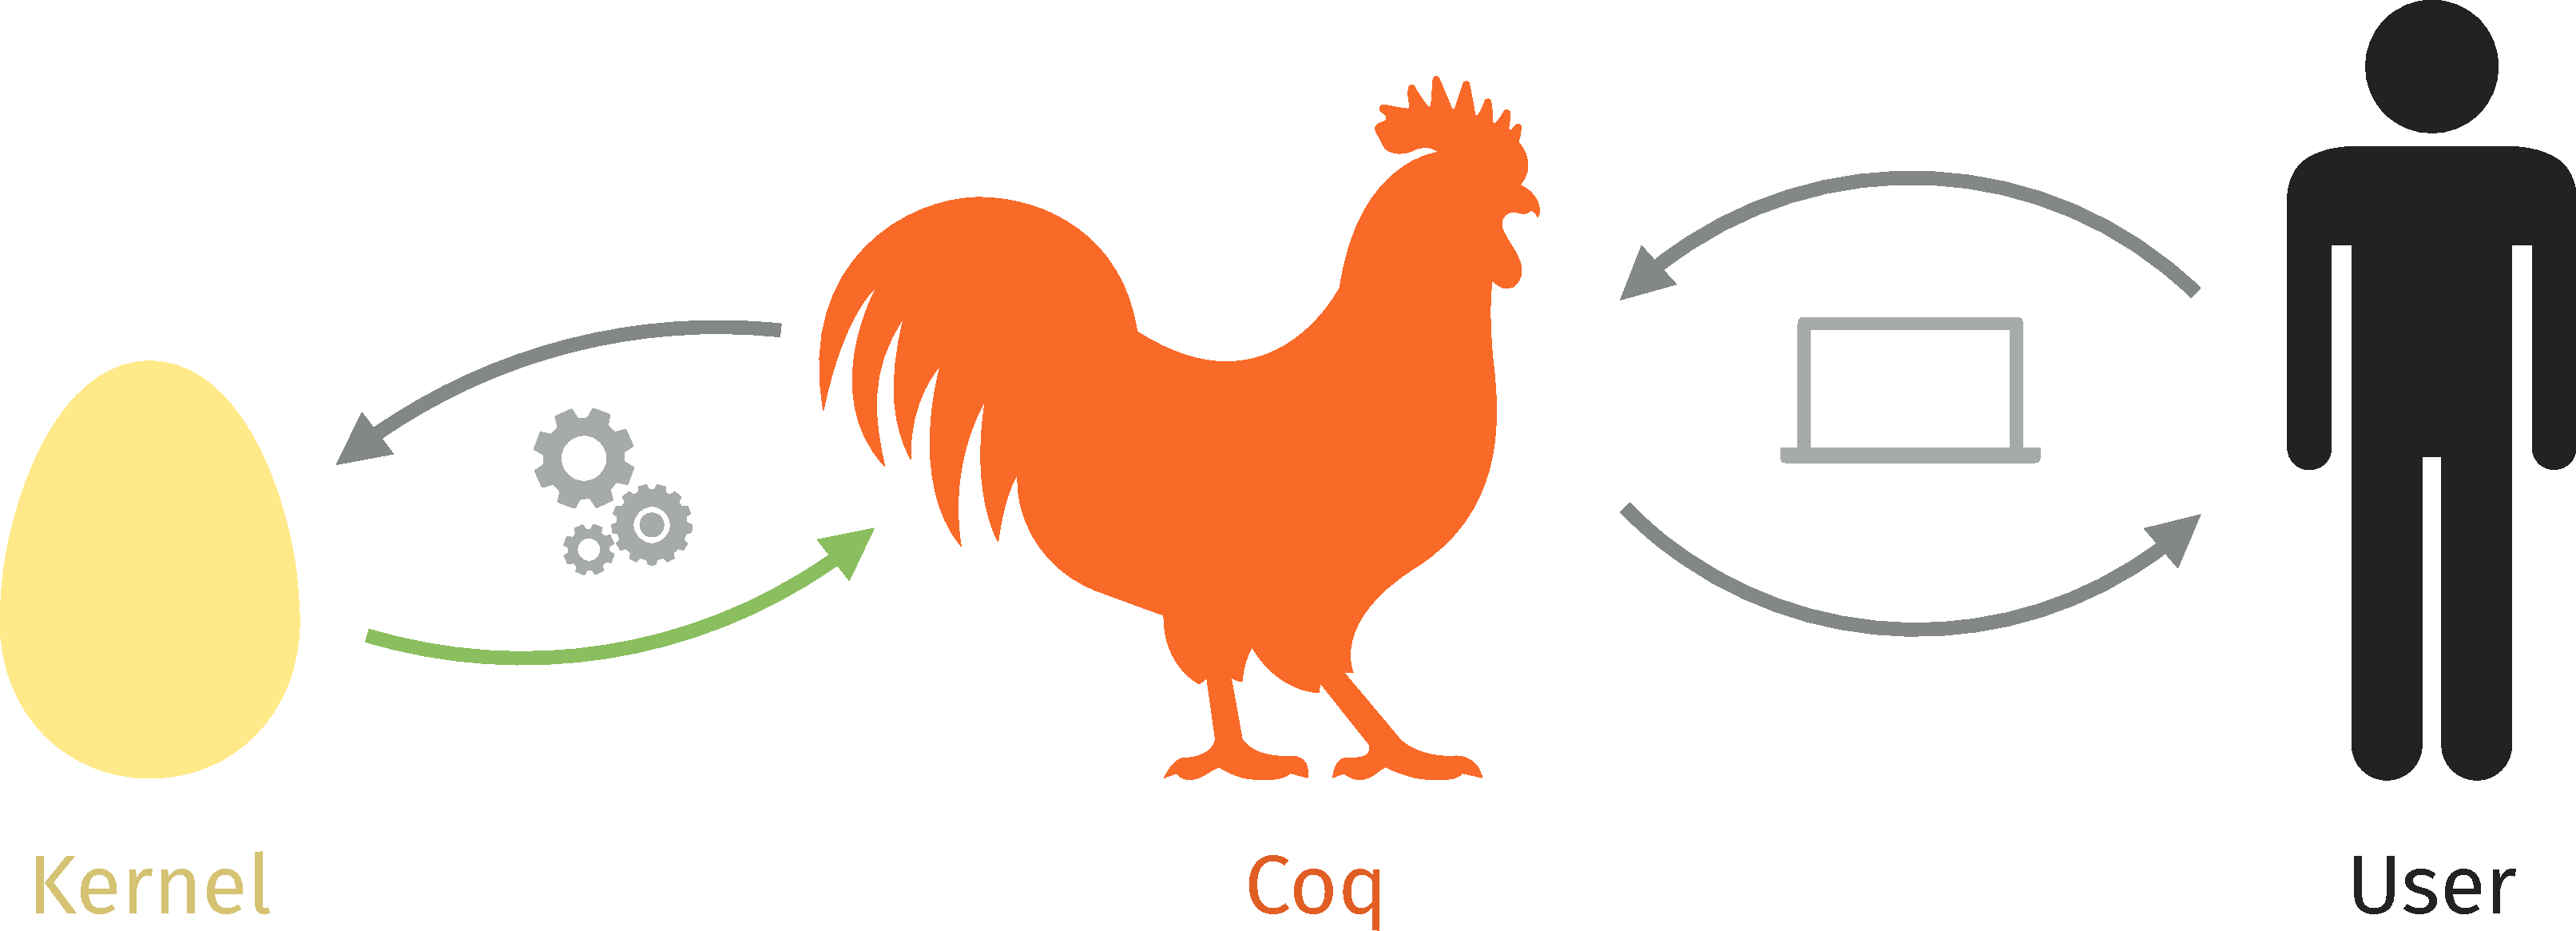
\includegraphics[width=0.99\textwidth]{coq-kernel.pdf}
\end{figure}

In this setting the kernel has to be kept as small as possible for inspection
by humans. In particular experimental features are dangerous in there.
\marginnote[0.1cm]{
  The interested reader can have a look at
  \url{https://github.com/coq/coq/blob/master/dev/doc/critical-bugs}
  where a list of critical bugs of \Coq is maintained.
}
Unfortunately, \Coq's kernel is not free of mistakes, and one critical bug has
been found roughly every year for the last two decades. Even then the kernel
presentation offers some damage control as it usually requires minor changes to
fix the problem.
In fact, those bugs are always related to the implementation rather than beeing
consistency issues of \acrshort{PCUIC}.

\acrshort{PCUIC} on the other hand seems more worthy of trust. The idea of our
project~\sidecite{sozeau2019coq} represents a paradigm shift: we propose to
replace the \acrshort{TCB} by a \acrfull{TTB}.
\begin{figure}[hb]
  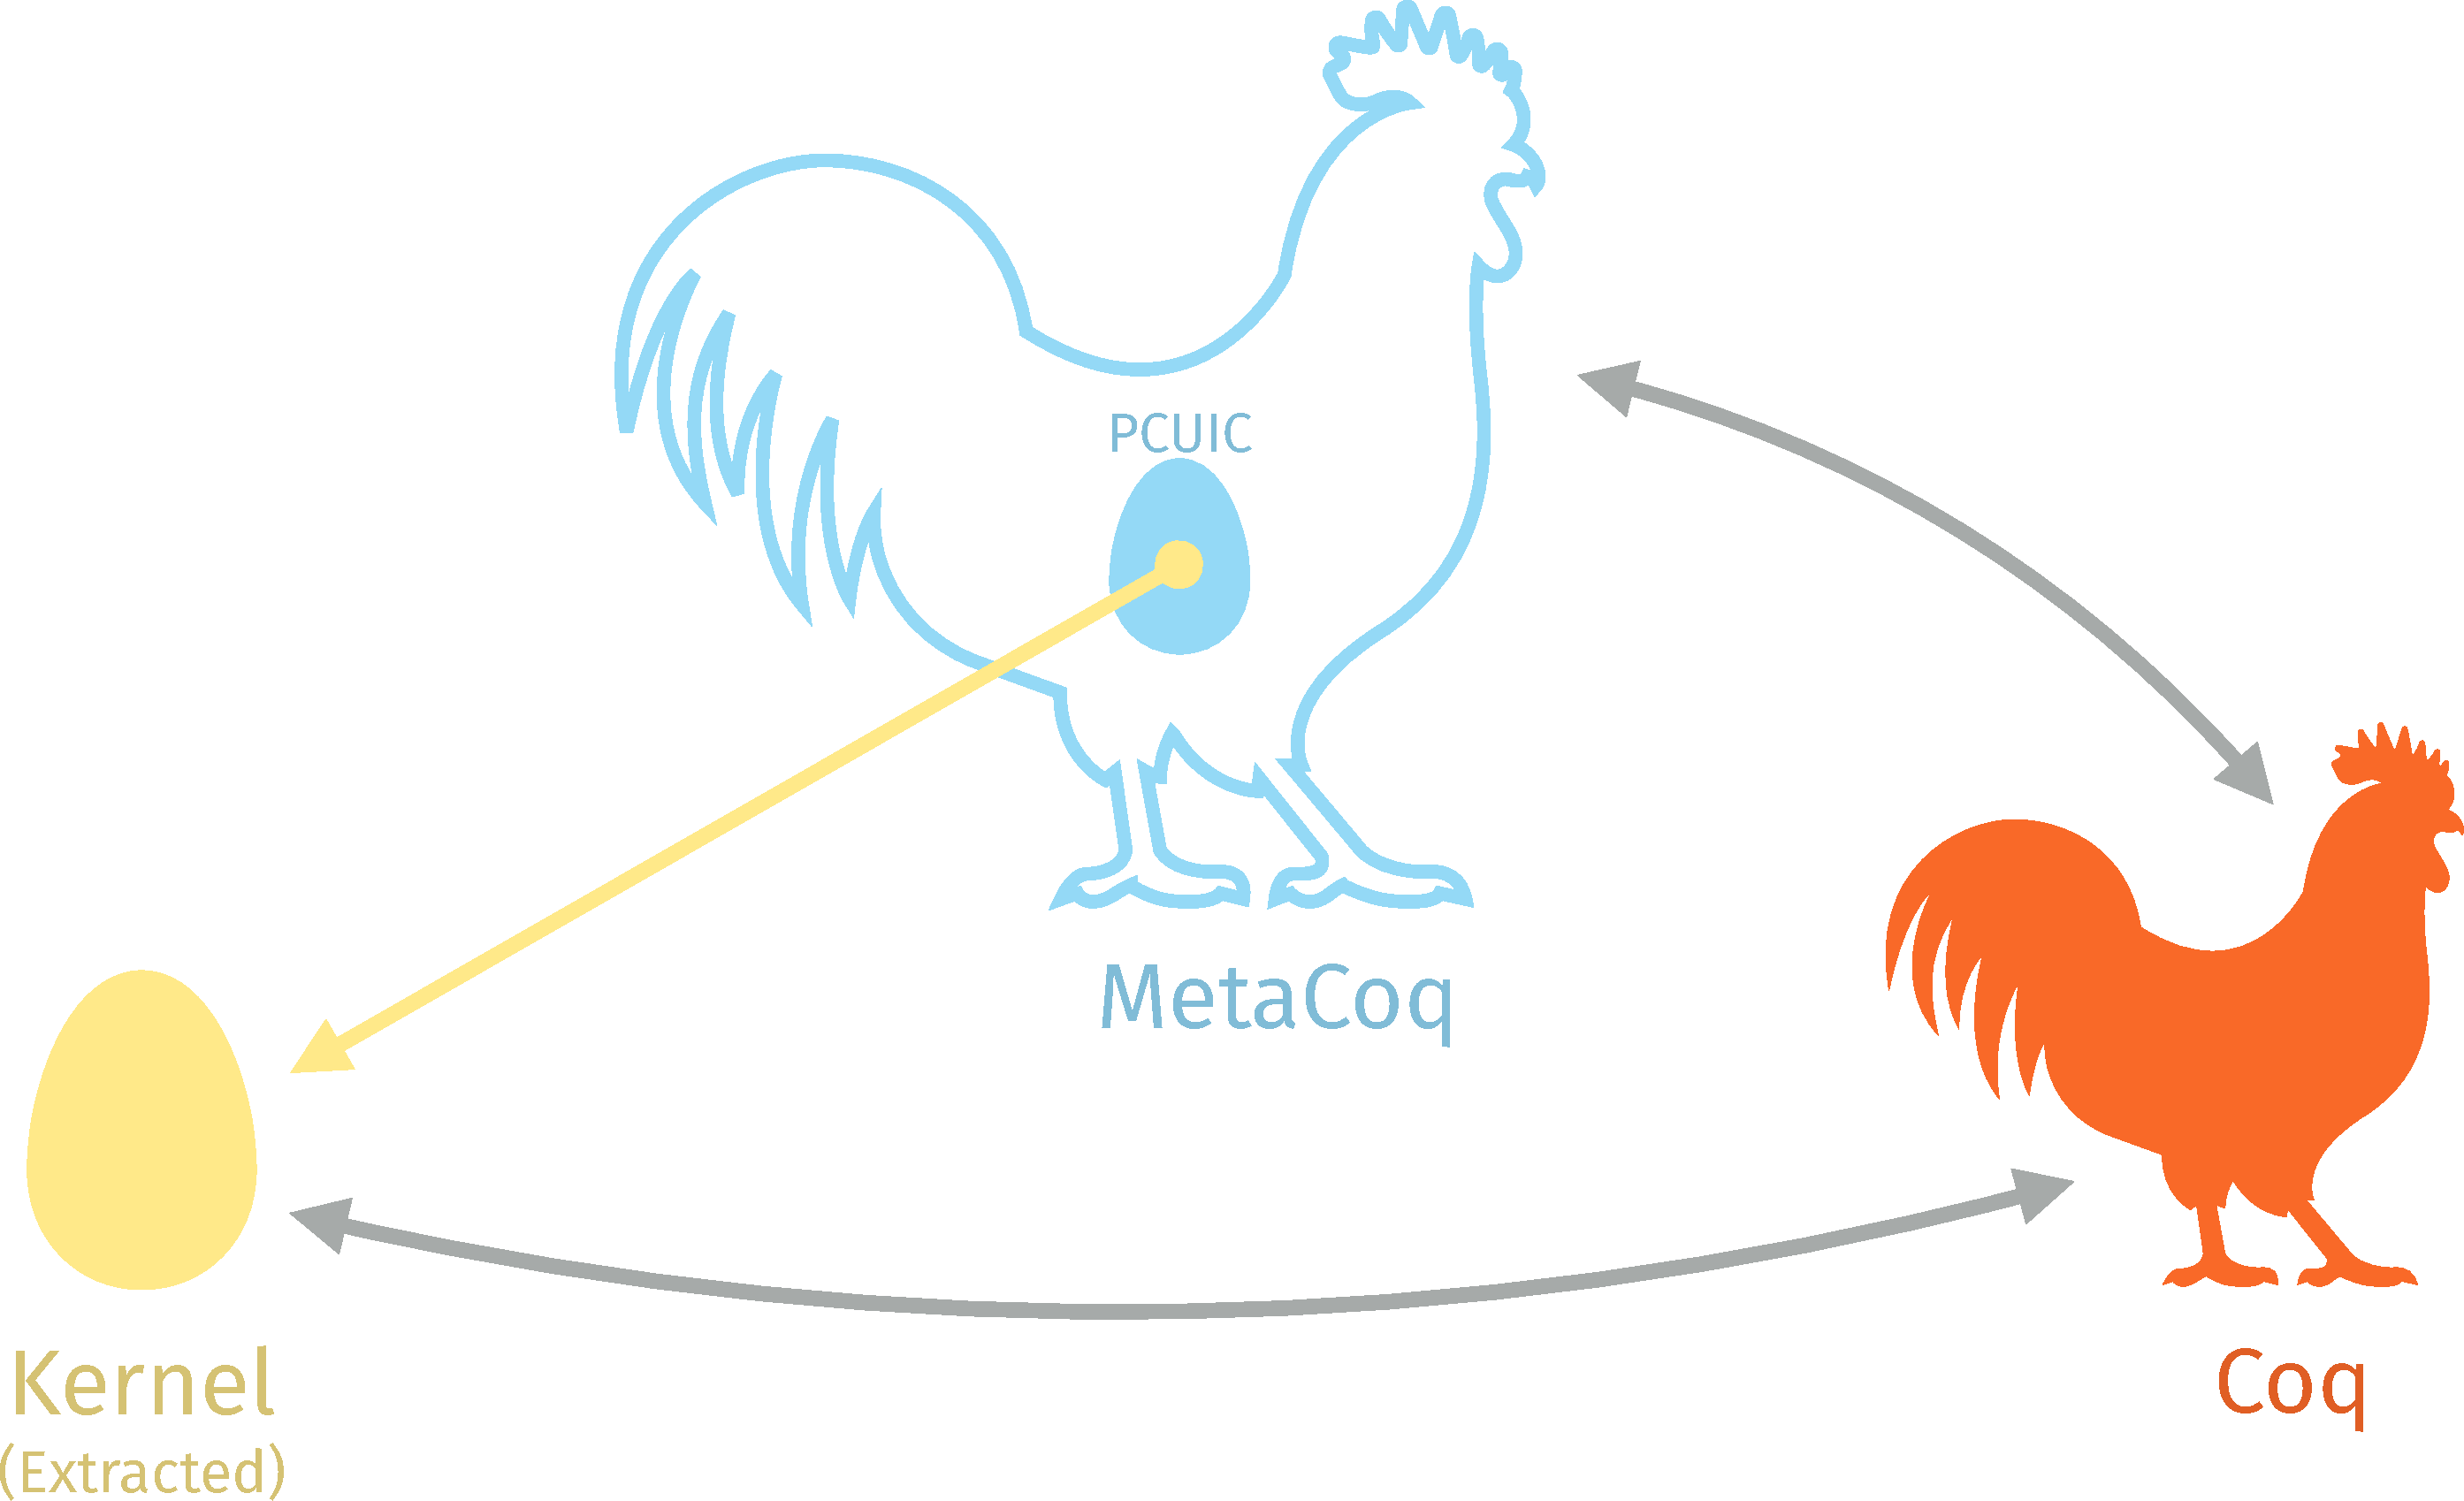
\includegraphics[width=0.7\textwidth]{trusted-theory.pdf}
\end{figure}

This time the idea is to rely on \MetaCoq which contains a specification of
\acrshort{PCUIC} to implement a verified kernel, assuming that the theory is
correct (hence the \acrshort{TTB}).
This \acrshort{TTB} is also kept to a minimum, only a few lemmata are part of it
now, and in time it should only consist in assuming strong normalisation.
The new kernel can be extracted to \Coq using its extraction
mechanism~\sidecite{Let2008} and it no longer has to be trusted. Of course this
requires trusting the extraction mechanism and even \Coq itself in which
\acrshort{PCUIC} is formalised.
The first point is mitigated by a verified extraction that is also part of the
project. The latter is more fundamental but I would like to argue that this is
\emph{not} entirely detrimental to our goal: the verified implementation is
still more detailed than the \ocaml implementation, in particular all the
invariants are made explicit; implementation and specification are now clearly
separated.

\marginnote[0.2cm]{
  See \nrefch{proof-theory} for more on Gödel's incompleteness theorems.
}
Note that we still have to rely on a \acrshort{TTB} because of Gödel's
incompleteness theorems which prevent us from proving consistency of
\Coq within \Coq.
\marginnote[0.1cm]{
  See \nrefch{desirable-props}.
}
This implies that we have to admit strong normalisation of the system, as it
would lead us to canonicity, hence consistency.
Thus, the assumption that the meta-theory enjoys the well-known assumed
properties is the main shortcoming of our formalisation. If those did not hold,
it would either raise a serious issue in \Coq's theory, or a problem in the
specification we made of it. For this last reason, the relatively small
specification we have is welcome.

\marginnote[1.2cm]{
  See \nrefch{flavours}.
}
Besides that, the theory of \acrshort{PCUIC} we specify and implement is a bit
simpler than that of \Coq: we use lists where arrays are involved and more
importantly we do not feature modules and template polymorphism.
The implementation also provides efficient universe constraint checking and
guard condition checking, we chose to remain abstract over those and simply
assume the existence of those in the specification: any implementation
satisfaying the specification can thus be plugged in. We use a rather naive
universe checker for now and do not provide any guard checking at all.
% \setchapterpreamble[u]{\margintoc}
\chapter{A specification of \Coq}
\labch{coq-spec}

In \nrefsec{coq-theory} I already talked about the type theory of \Coq we call
\acrshort{PCUIC} while in \nrefch{formalisation} you caught a glimpse of its
representation inside \Coq itself. In this chapter I will recall a few things
focusing on the points that were not discussed in those chapters like
representation of fixed-points and inductive types, as well as typing.

All this is the subject of~\sidecite{sozeau2019coq}.

\section{Syntax of \acrshort{PCUIC}}

In \MetaCoq, the syntax of \acrshort{PCUIC} is defined as the following
inductive type.
\begin{minted}{coq}
Inductive term :=
| tRel (n : nat)
| tSort (u : Universe.t)
| tProd (na : name) (A B : term)
| tLambda (na : name) (A t : term)
| tLetIn (na : name) (b B t : term)
| tApp (u v : term)
| tConst (k : kername) (ui : Instance.t)
| tInd (ind : inductive) (ui : Instance.t)
| tConstruct (ind : inductive) (n : nat) (ui : Instance.t)
| tCase
    (indn : inductive * nat)
    (p c : term)
    (brs : list (nat * term))
| tProj (p : projection) (c : term)
| tFix (mfix : mfixpoint term) (idx : nat)
| tCoFix (mfix : mfixpoint term) (idx : nat).
\end{minted}

I will not present again variables, \(\Pi\)-types, etc. and will focus on
the other constructors, for this I need to introduce the global environment.
% \mintinline{coq}{tConst}, \mintinline{coq}{tInd}, \mintinline{coq}{tConstruct},
% \mintinline{coq}{tCase}, \mintinline{coq}{tProj}, \mintinline{coq}{tFix}
% and \mintinline{coq}{tCoFix}.

\paradot{Global environment}

Just as for the translation presented in \arefpart{elim-reflection}, we have
a global environment \(\Sigma\) containing the axioms, definitions and
declarations of inductive types. Instead of using de Bruijn indices we use
strings to refer to these declarations. In fact, \mintinline{coq}{kername}
is simply a notation for \mintinline{coq}{string} which we use to lift
ambiguity as to its purpose.


\paradot{Universes}

Besides the global environment we have a set of universes with their
constraints. Indeed, although we usually present the hierarchy of universes in
\Coq using \(\Type_i\) with \(i \in \mathbb{N}\), the implementation is a bit
different in that universes are not fixed but floating.
\marginnote[0.65cm]{
  In \Coq, \(\Type_i\) is written \mintinline{coq}{Type@{i}}.
}
\begin{minted}{coq}
Type@{i} : Type@{j}
\end{minted}
holds in \Coq as long as the constraint \(i < j\) is satisfied but neither \(i\)
nor \(j\) correspond to natural numbers. Satisfying the constraints means that
there exist a valuation in the natural numbers preserving the constraints.
We also have local universes and constraints for polymorphic definitions;
universe instances (of type \mintinline{coq}{Instance.t}) are there to
substitute those for other universes.
Aside from \mintinline{coq}{Type}, we also represent \mintinline{coq}{Set}
and \mintinline{coq}{Prop}. We do not deal with \mintinline{coq}{SProp} yet.

\paradot{Constants}

\mintinline{coq}{tConst k ui} represents a definition or axiom declared in the
environment under name \mintinline{coq}{k}. Constant declarations are
inhabitants of the following record type.
\begin{minted}{coq}
Record constant_body := {
  cst_type : term ;
  cst_body : option term ;
  cst_universes : universes_decl
}.
\end{minted}
A constant comes with its type and an optional definition. Constants without
definitions are simply axioms.
The \mintinline{coq}{universes_decl} is there in case the constant happens to
be universe polymorphic.

\paradot{Inductive types}

\mintinline{coq}{tInd ind ui} represents an inductive type defined in the global
context. The type inductive is
\begin{minted}{coq}
Record inductive : Set := mkInd {
  inductive_mind : kername ;
  inductive_ind : nat
}.
\end{minted}
It is not just a \mintinline{coq}{kername} because inductive types can be
mutually defined: the kername points to the mutual block,
\mintinline{coq}{inductive_ind} points to one inductive in the block.
Note that this term refers to the inductive type, without its parameters or
indices. For vectors this would be
\begin{minted}{coq}
vec : Type -> nat -> Type
\end{minted}
In the global environment an inductive declaration provides the following
information.
\begin{minted}{coq}
Record mutual_inductive_body := {
  ind_finite    : recursivity_kind ;
  ind_npars     : nat ;
  ind_params    : context ;
  ind_bodies    : list one_inductive_body ;
  ind_universes : universes_decl ;
  ind_variance  : option (list Universes.Variance.t)
}.
\end{minted}
These informations include the number of parameters, the type of these
parameters in the form of a context and the universe declarations.
\mintinline{coq}{ind_variance} deals with variance of universes in the case
of cumulative inductive types.
The \mintinline{coq}{recursivity_kind} determines what kind of inductive type
we are building, this in fact include the usual inductive types, but also
record types and coinductive types.
Finally, \mintinline{coq}{ind_bodies} is a list of declarations for each of
the inductive types in the mutual block.
\begin{minted}{coq}
Record one_inductive_body := {
  ind_name  : ident ;
  ind_type  : term ;
  ind_kelim : sort_family ;
  ind_ctors : list (ident * term * nat) ;
  ind_projs : list (ident * term)
}.
\end{minted}
Each of those comes with its name and type.
\mintinline{coq}{ind_kelim} states in which univeres the definition can be
eliminated (in most cases inductive types living in \mintinline{coq}{Prop}
cannot be scrutinised to build terms in \mintinline{coq}{Type}).
Then we either have a list of constructors for (co)inductive types, or a list
of projections for (negative) records.

\paradot{Constructors}

\mintinline{coq}{tConstruct ind n ui} comes with \mintinline{coq}{ind} to point
to the right inductive type while \mintinline{coq}{n} tells us which constructor
it is.
For instance it would be \mintinline{coq}{0} for \mintinline{coq}{true} and
\mintinline{coq}{1} for \mintinline{coq}{false}.
Each constructor is given by a term of type
\begin{minted}{coq}
ident * term * nat
\end{minted}
as we saw in the previous paragraph. It consists in a name, a type and an arity.

\paradot{Pattern-matching}
\mintinline{coq}{tCase (ind, n) p c brs} is the representation of the
pattern-matching on \mintinline{coq}{c} of inductive type \mintinline{coq}{ind}
with \mintinline{coq}{n} parameters, return predicate \mintinline{coq}{p}
and branches \mintinline{coq}{brs}.
There is one branch for each constructor and it contains the arity of the
constructor and the term corresponding to the branch.

\paradot{Projections}
\mintinline{coq}{tProj p c} represents the projection \mintinline{coq}{p}
applied to term \mintinline{coq}{c}.
\begin{minted}{coq}
Definition projection :=
  inductive * nat * nat.
\end{minted}
A projection is described by the inductive (or rather record) to which it
belongs, the number of parameters of the record, and the index of the projected
argument. In the case of dependent pairs, the latter will be \mintinline{coq}{0}
for the first projection and \mintinline{coq}{1} for the second.

\paradot{Fixed-points}
Finally we have \mintinline{coq}{tFix mfix idx} representing fixed-points and
\mintinline{coq}{tCoFix mfix idx} for cofixed-points.
Like inductive types, fixed-points can be defined mutually, as such
\mintinline{coq}{mfix} is a list of (mutual) definitions:
\begin{minted}{coq}
Definition mfixpoint term :=
  list (def term).
\end{minted}
while \mintinline{coq}{idx} tells which one we are referring to.
Definitions which are given as
\begin{minted}{coq}
Record def term := mkdef {
  dname : name ;
  dtype : term ;
  dbody : term ;
  rarg  : nat
}.
\end{minted}
that is with a name, a type and a body (the definition itself).
The \mintinline{coq}{rarg} field points to the recursive argument of the
fixed-point.
For instance in
\begin{minted}{coq}
Fixpoint map {A B : Type} (f : A -> B) (l : list A) {struct l}
  : list B :=
  match l with
  | [] => []
  | x :: l => f x :: map f l
  end.
\end{minted}
the \mintinline{coq}{{struct l}} means that \mintinline{coq}{l} is the recursive
argument. That is all recursive calls must be structually decreasing on
\mintinline{coq}{l}. It is part of the syntax because \Coq uses it as a
syntactic guard to avoid unfolding fixed-points indefinitely: only when the
recursive argument is a constructor can the fixed-point be unfolded.

\paradot{Local environments}
Local environments or contexts are lists of declarations we write in \emph{snoc}
order:
\begin{itemize}
  \item \mintinline{coq}{[]} is the empty context;
  \item \mintinline{coq}{Γ ,, vass na A} extends \mintinline{coq}{Γ} with
  an \emph{assumption} variable of type \mintinline{coq}{A}, named
  \mintinline{coq}{na};
  \item \mintinline{coq}{Γ ,, vdef na a A} extends \mintinline{coq}{Γ} with
  a \emph{local definition} \mintinline{coq}{a} of type \mintinline{coq}{A},
  named \mintinline{coq}{na}.
\end{itemize}

Now that the syntax is out of the way we can move to the semantics.

\section{Semantics of \acrshort{PCUIC}}

There are two important properties defined on the syntax: reduction and typing.
The former being necessary for the latter as it is the base for conversion.

\subsection{Reduction}

We define reduction as a relation on terms, however, unlike for \acrshort{STL}
or many systems, because of constants and let-bindings which can be unfolded
to their definitions, the relation has to mention the global and local
environment. Note also that the relation is not functional, that is that the
reduction we define is not deterministic.

The inductive type of \(1\)-step reduction is
\begin{minted}{coq}
Inductive red1 (Σ : global_env) (Γ : context) :
  term -> term -> Type
\end{minted}
I will give the different constructors one by one, while explaining them,
focusing on the computation rules.

\paradot{\(\beta\)-reduction}
\begin{minted}{coq}
red_beta na t b a :
  red1 Σ Γ (tApp (tLambda na t b) a) (subst10 a b)
\end{minted}
This is the usual \(\beta\)-reduction rule, \mintinline{coq}{subst10 a b}
is just the term \mintinline{coq}{b} where the \(0\)-th variable is substituted
by \mintinline{coq}{a}.

\paradot{\(\zeta\)-reduction}
\begin{minted}{coq}
red_zeta na b t b' :
  red1 Σ Γ (tLetIn na b t b') (subst10 b b')
\end{minted}
This rule is similar to \(\beta\)-reduction, it states that the expression
\begin{minted}{coq}
let x := b in t x
\end{minted}
reduces to \mintinline{coq}{t b}.

\paradot{Local definition unfolding}
\begin{minted}{coq}
red_rel i body :
  option_map decl_body (nth_error Γ i) = Some (Some body) ->
  red1 Σ Γ (tRel i) (lift0 (S i) body)
\end{minted}
If the context contains some local definition \(x := t\) then the variable
\(x\) \emph{reduces} to \(t\). Because the definition makes sense in a
smaller context, it needs to be weakened, hence the \mintinline{coq}{lift}.

\paradot{\(\iota\)-reduction}
\marginnote[1.5cm]{
  \mintinline{coq}{mkApps} is a shortcut to apply a term to a list of arguments.
}
\begin{minted}{coq}
red_iota ind pars c u args p brs :
  red1 Σ Γ
    (tCase (ind, pars) p (mkApps (tConstruct ind c u) args) brs)
    (iota_red pars c args brs)
\end{minted}
Pattern-matching reduces when the term under scrutiny is a constructor
(potentially applied to some arguments).
\mintinline{coq}{iota_red} is defined as follows
\begin{minted}{coq}
Definition iota_red npar c args brs :=
  mkApps
    (snd (List.nth c brs (0, tDummy)))
    (List.skipn npar args).
\end{minted}
\mintinline{coq}{List.nth} takes a default value, so
\mintinline{coq}{(0, tDummy)} can be safely ignored. \mintinline{coq}{iota_red}
basically picks the branch corresponding to the constructor giving it the list
of indices \mintinline{coq}{List.skipn npar args}.

\paradot{Fixed-point unfolding}
\begin{minted}{coq}
red_fix mfix idx args narg fn :
  unfold_fix mfix idx = Some (narg, fn) ->
  is_constructor narg args = true ->
  red1 Σ Γ (mkApps (tFix mfix idx) args) (mkApps fn args)
\end{minted}
Here we can witness the syntactic guard I talked about when describing
fixed-points: when a fixed-point is applied to arguments such that its recursive
argument is an applied constructor, it can safely be unfolded.
\mintinline{coq}{unfold_fix mfix idx} returns the recursive argument
\mintinline{coq}{narg} and the body of the fixed-point \mintinline{coq}{fn}.

\paradot{Cofixed-point unfolding}
There are two rules to deal with unfolding of cofixed-points: one when it is
pattern-matched, the other when it is projected.
\begin{minted}{coq}
red_cofix_case ip p mfix idx args narg fn brs :
  unfold_cofix mfix idx = Some (narg, fn) ->
  red1 Σ Γ
    (tCase ip p (mkApps (tCoFix mfix idx) args) brs)
    (tCase ip p (mkApps fn args) brs)

red_cofix_proj p mfix idx args narg fn :
  unfold_cofix mfix idx = Some (narg, fn) ->
  red1 Σ Γ
    (tProj p (mkApps (tCoFix mfix idx) args))
    (tProj p (mkApps fn args))
\end{minted}
The are very similar to fixed-points except this time there is no syntactic
guard with respect to a recursive argument.

\paradot{\(\delta\)-reduction}
\begin{minted}{coq}
red_delta c decl body (isdecl : declared_constant Σ c decl) u :
  decl.(cst_body) = Some body ->
  red1 Σ Γ (tConst c u) (subst_instance_constr u body)
\end{minted}
A constant can reduce to its definition in the global environment (if it has
one, \ie if it is not an axiom). Since the definition is potentially universe
polymorphic, we instantiate its universes with the one the constant was used
with.

\paradot{Projection}
\begin{minted}{coq}
red_proj i pars narg args k u arg:
  nth_error args (pars + narg) = Some arg ->
  red1 Σ Γ
    (tProj (i, pars, narg) (mkApps (tConstruct i k u) args))
    arg
\end{minted}
When a constructor of a record (that is the record is given with its fields) is
projected, it reduces to the corresponding field.

\paradot{Congruence rules}
All remaining rules are congruence rules we have for instance the two congruence
rules for \mintinline{coq}{tLambda}:
\begin{minted}{coq}
| abs_red_l na M M' N :
    red1 Σ Γ M M' ->
    red1 Σ Γ (tLambda na M N) (tLambda na M' N)

| abs_red_r na M M' N :
    red1 Σ (Γ ,, vass na N) M M' ->
    red1 Σ Γ (tLambda na N M) (tLambda na N M')
\end{minted}
They state that you can reduce either subterm.

\subsection{Conversion}

Unlike \Agda, conversion in \Coq is not typed but rather based primarily on
reduction. Its definition is the following, corresponding basically to the
reflexive, symmetric and transitive closure of reduction:
\marginnote[1cm]{
  Here \mintinline{coq}{Σ} is a pair comprised of a global environment and the
  universe declarations.
}
\begin{minted}{coq}
Inductive conv Σ Γ : term -> term -> Type :=
| conv_refl t u :
    eq_term (global_ext_constraints Σ) t u ->
    Σ ;;; Γ |- t = u

| conv_red_l t u v :
    red1 Σ Γ t v ->
    Σ ;;; Γ |- v = u ->
    Σ ;;; Γ |- t = u

| conv_red_r t u v :
    Σ ;;; Γ |- t = v ->
    red1 (fst Σ) Γ u v ->
    Σ ;;; Γ |- t = u

where " Σ ;;; Γ |- t = u " := (@conv _ Σ Γ t u) : type_scope.
\end{minted}

In terms of inference rules this would be written
\begin{mathpar}
  \infer
    {t =_{\alpha} u}
    {\Sigma ; \Ga \vdash t \equiv u}
  %

  \infer
    {
      \Sigma ; \Ga \vdash t \red v \\
      \Sigma ; \Ga \vdash v \equiv u
    }
    {\Sigma ; \Ga \vdash t \equiv u}
  %

  \infer
    {
      \Sigma ; \Ga \vdash t \equiv v \\
      \Sigma ; \Ga \vdash u \red v
    }
    {\Sigma ; \Ga \vdash t \equiv u}
  %
\end{mathpar}
This is similar except that we do not merely use \(\alpha\)-conversion in the
reflexive case, we also equate the terms up to universes.
Indeed sometimes, two universes may be syntactically different but still be the
same like \(i\) and \(j\) with constraints \(i \le j\) and \(j \le i\).

This becomes more apparent in the cumulativity definition.
\begin{minted}{coq}
Inductive cumul Σ Γ : term -> term -> Type :=
| cumul_refl t u :
    leq_term (global_ext_constraints Σ) t u ->
    Σ ;;; Γ |- t <= u

| cumul_red_l t u v :
    red1 Σ Γ t v ->
    Σ ;;; Γ |- v <= u ->
    Σ ;;; Γ |- t <= u

| cumul_red_r t u v :
    Σ ;;; Γ |- t <= v ->
    red1 Σ Γ u v ->
    Σ ;;; Γ |- t <= u

where " Σ ;;; Γ |- t <= u " := (cumul Σ Γ t u) : type_scope.
\end{minted}

\begin{mathpar}
  \infer
    {t \le_{\alpha} u}
    {\Sigma ; \Ga \vdash t \cumul u}
  %

  \infer
    {
      \Sigma ; \Ga \vdash t \red v \\
      \Sigma ; \Ga \vdash v \cumul u
    }
    {\Sigma ; \Ga \vdash t \cumul u}
  %

  \infer
    {
      \Sigma ; \Ga \vdash t \cumul v \\
      \Sigma ; \Ga \vdash u \red v
    }
    {\Sigma ; \Ga \vdash t \cumul u}
  %
\end{mathpar}
Of course this time it is not symmetric. We break symmetry by using
\mintinline{coq}{leq_term} to perform \(\alpha\)-equlity up to universes.
In a sense this is what does all the work regarding cumulativity.

We define \mintinline{coq}{eq_term} and \mintinline{coq}{leq_term} at the same
time using a more general definition.
\marginnote[0.5cm]{
  \mintinline{coq}{φ} represents the universe constraints.
  \mintinline{coq}{eq_universe} and \mintinline{coq}{leq_universe} are relations
  on universes with self-explanatory names.
}
\begin{minted}{coq}
Definition eq_term φ :=
  eq_term_upto_univ (eq_universe φ) (eq_universe φ).

Definition leq_term φ :=
  eq_term_upto_univ (eq_universe φ) (leq_universe φ).
\end{minted}

The definition of \mintinline{coq}{eq_term_upto_univ} is rather long so I will
give an excerpt of it.
\begin{minted}{coq}
Inductive eq_term_upto_univ
  (Re Rle : Universe.t -> Universe.t -> Prop)
  : term -> term -> Type :=

| eq_Rel n  :
    eq_term_upto_univ Re Rle (tRel n) (tRel n)

| eq_Sort s s' :
    Rle s s' ->
    eq_term_upto_univ Re Rle (tSort s) (tSort s')

| eq_App t t' u u' :
    eq_term_upto_univ Re Rle t t' ->
    eq_term_upto_univ Re Re u u' ->
    eq_term_upto_univ Re Rle (tApp t u) (tApp t' u')

| eq_Const c u u' :
    R_universe_instance Re u u' ->
    eq_term_upto_univ Re Rle (tConst c u) (tConst c u')

| eq_Prod na na' a a' b b' :
    eq_term_upto_univ Re Re a a' ->
    eq_term_upto_univ Re Rle b b' ->
    eq_term_upto_univ Re Rle (tProd na a b) (tProd na' a' b')

(* ... *)
.
\end{minted}
As you can see, when comparing sorts we simply compare the universes with
\mintinline{coq}{Rle}. Otherwise, we simply compare the subterms with the same
relations. There is the exception of domains however, indeed they are in
contravariant positions and as such they should need to be compared in reverse
order. In \Coq we simply use conversion rather that cumulativity in
contravariant positions:
\begin{mathpar}
  \infer
    {
      A =_\alpha A' \\
      B \le_\alpha B'
    }
    {\Pi (x:A). B \le_\alpha \Pi (x:A'). B'}
  %
\end{mathpar}
We also compare universe instances for polymorphic constants.

\paradot{About \(\eta\)}
\reminder[-0.7cm]{\(\eta\)-expansion}{
  \(\eta\)-expansion is defined as follows
  \[
    t \red_\eta \lambda x.\ t\ x
  \]
}
\Coq supports \(\eta\)-expansion in the conversion. In a typed setting like
\Agda's conversion it is rather easy to add it. In \Agda the conversion rule can
be given as
\[
  \infer
    { }
    {\Ga \vdash t \equiv \lambda x.\ t\ x : \Pi (x:A). B}
  %
\]
or even in a more directed way as
\[
  \infer
    {\Ga, x:A \vdash f\ x \equiv g\ x : B}
    {\Ga \vdash f \equiv g : \Pi (x:A). B}
  %
\]
In an untyped setting the question is a bit more complex, we have several
candidates but are struggling to find a formulation that lets us preserve good
properties about conversion/cumulativity without going through to much trouble.

\subsection{Typing}

Again, typing is defined inductively.
\begin{minted}{coq}
Inductive typing (Σ : global_env_ext) (Γ : context)
  : term -> term -> Type
(* ... *)
where " Σ ;;; Γ |- t : T " := (typing Σ Γ t T) : type_scope.
\end{minted}
I will go over the rules one by one.

\paradot{Variables}
\begin{minted}{coq}
type_Rel n decl :
  All_local_env (lift_typing typing Σ) Γ ->
  nth_error Γ n = Some decl ->
  Σ ;;; Γ |- tRel n : lift0 (S n) decl.(decl_type)
\end{minted}
Herein \mintinline{coq}{All_local_env (lift_typing typing Σ) Γ} will later on
be written \mintinline{coq}{wf_local Σ Γ}, it corresponds to well-formedness
of the local environment \(\Sigma \vdash \Ga\). This basically means that
the types and local definitions in it are well-typed.
\begin{minted}{coq}
nth_error Γ n = Some decl
\end{minted}
verifies that the variable
\mintinline{coq}{n} corresponds to a declaration in \mintinline{coq}{Γ}.
The type of the variable is thus the type stored in this declaration. As always
it has to be \emph{lifted}, \ie weakened to account for the declarations
that were added successively in \mintinline{coq}{Γ}.

\paradot{Sorts}
\begin{minted}{coq}
type_Sort l :
  wf_local Σ Γ ->
  LevelSet.In l (global_ext_levels Σ) ->
  Σ ;;; Γ |- tSort (Universe.make l) : tSort (Universe.super l)
\end{minted}
For universes we once again require to local environment to be well-formed.
The universe should also make sense in the global environment, in which case it
is typed in its successor universe.

\paradot{\(\Pi\)-types}
\begin{minted}{coq}
type_Prod na A B s1 s2 :
  Σ ;;; Γ |- A : tSort s1 ->
  Σ ;;; Γ ,, vass na A |- B : tSort s2 ->
  Σ ;;; Γ |- tProd na A B : tSort (sort_of_product s1 s2)
\end{minted}
\(\Pi (x:A).B\) is well-typed if \(A\) and \(B\) are well-typed too.
The \(\Pi\)-types lives in another universe computed from the universes of
\(A\) and \(B\), if those are \(\Type_i\) and \(\Type_j\) this will be
\(\Type_{\max\ i\ j}\) but if the second is \(\Prop\), then the \(\Pi\)-type
lives in \(\Prop\) too thanks to impredicativity.

\paradot{\(\lambda\)-abstractions}
\begin{minted}{coq}
type_Lambda na A t s1 B :
  Σ ;;; Γ |- A : tSort s1 ->
  Σ ;;; Γ ,, vass na A |- t : B ->
  Σ ;;; Γ |- tLambda na A t : tProd na A B
\end{minted}

\paradot{let-bindings}
\begin{minted}{coq}
type_LetIn na b B t s1 A :
  Σ ;;; Γ |- B : tSort s1 ->
  Σ ;;; Γ |- b : B ->
  Σ ;;; Γ ,, vdef na b B |- t : A ->
  Σ ;;; Γ |- tLetIn na b B t : tLetIn na b B A
\end{minted}
Here we see the interesting fact that let-bindings are typed by let-bindings
themselves. That is because the type \mintinline{coq}{A} also makes sense in
\mintinline{coq}{Γ ,, vdef na b B} that is an environment extended with a local
definition.

\paradot{Application}
\begin{minted}{coq}
type_App t na A B u :
  Σ ;;; Γ |- t : tProd na A B ->
  Σ ;;; Γ |- u : A ->
  Σ ;;; Γ |- tApp t u : B{0 := u}
\end{minted}
Here \mintinline{coq}{B{0 := u}} stands for \mintinline{coq}{B} where the
\(0\)-th variable is substituted by \mintinline{coq}{u}.

\paradot{Constants}
\begin{minted}{coq}
type_Const k u :
  wf_local Σ Γ ->
  forall d (isdecl : declared_constant Σ.1 k d),
  consistent_instance_ext Σ d.(cst_universes) u ->
  Σ ;;; Γ |- tConst k u : subst_instance_constr u d.(cst_type)
\end{minted}
The rule is a complicated way of saying that if the constant
\mintinline{coq}{k} is declared in the global environment and used with
a consistent instance of universes, it has the type prescribed by
\mintinline{coq}{Σ} instantiated with those universes.

\paradot{Inductive types}
\begin{minted}{coq}
type_Ind ind u :
  wf_local Σ Γ ->
  forall md id (isdecl : declared_inductive Σ.1 md ind id),
  consistent_instance_ext Σ md.(ind_universes) u ->
  Σ ;;; Γ |- tInd ind u : subst_instance_constr u id.(ind_type)
\end{minted}
This rule is pretty similar to constants because without their constructors,
inductive types are really just constants.

\paradot{Constructors}
\begin{minted}{coq}
type_Construct ind i u :
  wf_local Σ Γ ->
  forall md id cd
    (isdecl : declared_constructor Σ.1 md id (ind, i) cd),
    consistent_instance_ext Σ md.(ind_universes) u ->
    Σ ;;; Γ |- tConstruct ind i u :
               type_of_constructor md cd (ind, i) u
\end{minted}
A constructor is well-typed when the inductive it refers to is declared and
the constructor itself is declared in it.
\mintinline{coq}{type_of_constructor} recovers the corresponding type and put it
in context, substituting the universes.

\paradot{Pattern-matching}
\begin{minted}{coq}
type_Case in u p c brs args :
  let ind := in.1 in
  let npar := in.2 in
  forall md id (isdecl : declared_inductive Σ.1 md ind id),
  md.(ind_npars) = npar ->
  let params := List.firstn npar args in
  forall ps pty,
  build_case_predicate_type ind md id params u ps = Some pty ->
  Σ ;;; Γ |- p : pty ->
  leb_sort_family (universe_family ps) id.(ind_kelim) ->
  Σ ;;; Γ |- c : mkApps (tInd ind u) args ->
  forall btys,
  map_option_out (build_branches_type ind md id params u p) =
  Some btys ->
  All2 (fun br bty =>
    (br.1 = bty.1) *
    (Σ ;;; Γ |- br.2 : bty.2) *
    (Σ ;;; Γ |- bty.2 : tSort ps)
  ) brs btys ->
  Σ ;;; Γ |- tCase in p c brs :
             mkApps p (skipn npar args ++ [c])
\end{minted}
This rule is rather hairy. We verify that the inductive type given for the
scrutinee is declared; we verify that the return predicate has the right type and
is in a sort which can be eliminated to; we verify that the scrutinee is indeed
typed in the inductive type and we recover the indices from its type, they will
be used in the return type; finally we verify that each branch is well-typed
using the other information.

\paradot{Projection}
\begin{minted}{coq}
type_Proj p c u :
  forall md id pd
    (isdecl : declared_projection Σ.1 md id p pd) args,
    Σ ;;; Γ |- c : mkApps (tInd (fst (fst p)) u) args ->
    #|args| = ind_npars md ->
    let ty := snd pd in
    Σ ;;; Γ |- tProj p c :
    subst0 (c :: List.rev args) (subst_instance_constr u ty)
\end{minted}
As usual we verify that the projection is declared and corresponds to a declared
record type. The projected term must be of that record type, where universes
are instantited. The projection has then the type of the corresponding field
with these universes.

\paradot{Fixed-points}
\begin{minted}{coq}
type_Fix mfix n decl :
  fix_guard mfix ->
  nth_error mfix n = Some decl ->
  wf_local Σ Γ ->
  All (fun d => {s & Σ ;;; Γ |- d.(dtype) :  tSort s}) mfix ->
  All (fun d =>
    (Σ ;;; Γ ,,, fix_context mfix |-
      d.(dbody) :
      lift0 #|fix_context mfix| d.(dtype)
    ) *
    (isLambda d.(dbody) = true)
  ) mfix ->
  Σ ;;; Γ |- tFix mfix n : decl.(dtype)
\end{minted}
A fixed-point is well-typed if all the types of the different mutual functions
are sorted (\ie are typed in a universe) and if the bodies have their ascribed
types in the context extended with the mutual functions (the bodies can refer
to other functions or do a recusrive call to themselves).
We also ask that each body is at least a \(\lambda\)-abstraction to make sure it
takes at least one argument explicitly.
The interesting point however is
\begin{minted}{coq}
fix_guard mfix
\end{minted}
This is our own representation of the guard condition ensuring that the
fixed-point is terminating. As the guard condition of \Coq is rather complicated
and perhaps ad-hoc we instead assume we have such a guard condition satisfying
some properties and work with it in generality.
For this we use axioms
\begin{minted}{coq}
Axiom fix_guard : mfixpoint term -> bool.

Axiom fix_guard_red1 :
  forall Σ Γ mfix mfix' idx,
    fix_guard mfix ->
    red1 Σ Γ (tFix mfix idx) (tFix mfix' idx) ->
    fix_guard mfix'.

(* ... *)
\end{minted}
which has the drawback that they cannot be instantiated with actual guard
conditions. We will probably change this at some point in the future.

\paradot{Cofixed-points}
\begin{minted}{coq}
type_CoFix mfix n decl :
  allow_cofix ->
  nth_error mfix n = Some decl ->
  wf_local Σ Γ ->
  All (fun d => {s & Σ ;;; Γ |- d.(dtype) :  tSort s}) mfix ->
  All (fun d =>
    Σ ;;; Γ ,,, fix_context mfix |-
      d.(dbody) :
      lift0 #|fix_context mfix| d.(dtype)
  ) mfix ->
  Σ ;;; Γ |- tCoFix mfix n : decl.(dtype)
\end{minted}
Cofixed-points are pretty similar to fixed-points except we do not even check
productivity, so that is still something that we need to work on.

\paradot{Cumulativity}
\begin{minted}{coq}
type_Cumul t A B :
  Σ ;;; Γ |- t : A ->
  (isWfArity typing Σ Γ B + {s & Σ ;;; Γ |- B : tSort s}) ->
  Σ ;;; Γ |- A <= B ->
  Σ ;;; Γ |- t : B
\end{minted}
The cumulativity rule is mostly unsurprising, if \(t : A\) and \(A \cumul B\)
then \(t : B\). As I have showed several times we require \(B\) to be
well-formed because conversion is untyped.
The way it is written here might be surprising however: we ask for the existence
of a sort typing \(B\) \emph{or} that \(B\) is a well-formed \emph{arity}.
This is an oddity of \Coq coming from the presence of so-called
\emph{algebraic universes} consisting of things such as \(i+1\) or
\(\max\ i\ j\). These universes should only appear on the right-hand side of
the colon, \ie in types.
An arity is a well-formed quantification over a universe that may be
algebraic. As those can appear in types, we allow them in the cumulativity
rule.
This peculiar aspect can be mostly ignored for the rest of this document,
and well-formedness of types can be thought of as the usual.


Note that I did not talk about typing of environments, local and global, but
they of course are also specified in the formalisation.
For inductive type declarations there is another guard condition that we
axiomatise:
\begin{minted}{coq}
Axiom ind_guard : mutual_inductive_body -> bool.
\end{minted}
In \Coq this is implemented as the strict positivity condition but we once again
remain abstract and simply ask for some way of determining if an inductive type
is well-founded.
These axioms will become meaningful when we reach the question of strong
normalisation in \nrefch{coq-meta-theory}.
% \setchapterpreamble[u]{\margintoc}
\chapter{Meta-theoretical properties}
\labch{coq-meta-theory}

\marginnote[0.5cm]{
  Most of these properties are defined in \nrefch{desirable-props}.
}
Before we can formalise the type checker, we need to develop some of the
meta-theory. In particular the type checker relies on subject reduction,
confluence and strong normalisation of the reduction.
As I already said in \nrefch{coq-overview}, these properties can be part of
the trusted base (and some of them like strong normalisation have to be in it
lest we prove consistency of \Coq whithin \Coq). Moreover they are not the
subject of this work. I will thus focus on their statements and not their
potential proofs, those are explained in~\sidecite{sozeau2019coq} or will be
in upcoming publications regarding the \MetaCoq project.

\paradot{Substitutivity and weakening}

Weakening and substitution preserve typing, a fact which we prove rather early
in the development. Such statements cannot really be assumed anyway since it is
really easy to make mistakes while manipulating de Bruijn indices.

The weakening theorem is rather simple:
\begin{minted}{coq}
Lemma weakening :
  forall Σ Γ Γ' (t : term) T,
    wf Σ ->
    wf_local Σ (Γ ,,, Γ') ->
    Σ ;;; Γ |- t : T ->
    Σ ;;; Γ ,,, Γ' |- lift0 #|Γ'| t : lift0 #|Γ'| T.
\end{minted}
It asks for the global environment and the extended local environment to make
sense as a precondition.

Substitution is slightly more complex
\begin{minted}{coq}
Lemma substitution :
  forall Σ Γ Γ' s Δ (t : term) T,
    wf Σ ->
    subslet Σ Γ s Γ' ->
    Σ ;;; Γ ,,, Γ' ,,, Δ |- t : T ->
    Σ ;;; Γ ,,, subst_context s 0 Δ |-
      subst s #|Δ| t : subst s #|Δ| T.
\end{minted}
This time we are replacing a bunch of variables at once using parallel
substitutions. Not only the term and type, but also the context that was built
on top of the substituted variables are substituted.
Unlike weakening, the substitution itself needs to be well-typed, this is
defined as follows.
\begin{minted}{coq}
Inductive subslet {cf:checker_flags} Σ (Γ : context)
  : list term -> context -> Type :=

| emptyslet :
    subslet Σ Γ [] []

| cons_let_ass Δ s na t T :
    subslet Σ Γ s Δ ->
    Σ ;;; Γ |- t : subst0 s T ->
    subslet Σ Γ (t :: s) (Δ ,, vass na T)

| cons_let_def Δ s na t T :
    subslet Σ Γ s Δ ->
    Σ ;;; Γ |- subst0 s t : subst0 s T ->
    subslet Σ Γ (subst0 s t :: s) (Δ ,, vdef na t T).
\end{minted}
Unlike substitution typing I presented earlier this needs to account for local
definitions (\ie let-bindings) in the environment.
In a more understable language this becomes
\marginnote[1cm]{
  This time I write \(\Ga \vdash \sigma : \D\) were earlier I wrote
  \(\sigma : \Ga \to \D\). This is because in this case \(\sigma\) is a list
  of terms.
}
\begin{mathpar}
  \infer
    { }
    {\Sigma ; \Ga \vdash \bullet : \ctxempty}
  %

  \infer
    {
      \Sigma ; \Ga \vdash \sigma : \D \\
      \Sigma ; \Ga \vdash t : A[\sigma]
    }
    {\Sigma ; \Ga \vdash \sigma, x \sto t : \D, x:A}
  %

  \infer
    {
      \Sigma ; \Ga \vdash \sigma : \D \\
      \Sigma ; \Ga \vdash t[\sigma] : A[\sigma]
    }
    {\Sigma ; \Ga \vdash \sigma, x \sto t[\sigma] : \D, x : A \coloneqq t}
  %
\end{mathpar}
Notice how the term of the substitution is forced when it targets a definition,
this is reassuring because a substitution should not overwrite definitions.

\paradot{Confluence}

Confluence is an important result that we have on \Coq's theory. In particular
it allows us to simplify greatly what it means to be convertible.
Indeed, right now, conversion involves reduction going in both directions so
that \(u\) and \(v\) can be convertible by something like the following picture.
\begin{center}
  \begin{tikzpicture}[baseline=(u.base), node distance=1cm]
    \node (u) { \(u\) } ;
    \node (d1) [above right = of u] {} ;
    \node (d2) [below right = of d1] {} ;
    \node (d3) [above right = of d2] {} ;
    \node (v) [below right = of d3] { \(v\) } ;
    \path (d1.center) edge[to*, tred] (u) ;
    \path (d1.center) edge[to*, tred] (d2) ;
    \path (d3.center) edge[to*, tred] (d2) ;
    \path (d3.center) edge[to*, tred] (v) ;
  \end{tikzpicture}
\end{center}
Thanks to confluence this picture can be completed into
\begin{center}
  \begin{tikzpicture}[baseline=(u.base), node distance=1cm]
    \node (u) { \(u\) } ;
    \node (d1) [above right = of u.center] {} ;
    \node (d2) [below right = of d1.center] {} ;
    \node (d3) [above right = of d2.center] {} ;
    \node (v) [below right = of d3.center] { \(v\) } ;
    \node (a) [below right = of u.center] {} ;
    \node (b) [below right = of d2.center] {} ;
    \node (c) [below right = of a.center] {} ;
    \path (d1.center) edge[to*, tred] (u) ;
    \path (d1.center) edge[to*, tred] (d2) ;
    \path (d3.center) edge[to*, tred] (d2) ;
    \path (d3.center) edge[to*, tred] (v) ;
    \path (u) edge[to*, tred, dashed] (a) ;
    \path (d2.center) edge[to*, tred, dashed] (a) ;
    \path (d2.center) edge[to*, tred, dashed] (b) ;
    \path (v) edge[to*, tred, dashed] (b) ;
    \path (a.center) edge[to*, tred, dashed] (c) ;
    \path (b.center) edge[to*, tred, dashed] (c) ;
  \end{tikzpicture}
\end{center}
This means that we can only regard conversion as \(u\) and \(v\) reducing to
the same term (up to names and universes).

\paradot{Context conversion}

This is property that I did not mention before: context conversion states that
you can replace a context in a judgment by another context where all types
and definitions are convertible to the original one.
This will often be used to replace \(\Ga, x:A\) by \(\Ga, x:A'\) with
\(A \equiv A'\) but is proven in full generality.

\paradot{Validity}

In \acrshort{PCUIC}, validity differs from the usual because of arities.
\begin{minted}{coq}
Lemma validity_term :
  forall Σ Γ t T,
    wf Σ ->
    Σ ;;; Γ |- t : T ->
    isWfArity_or_Type Σ Γ T.
\end{minted}
As you can see, \mintinline{coq}{T} is guaranteed to either be a type (as in
be typed in a universe) or a well-formed arity.

\paradot{Subject reduction}

At the time of writing, subject reduction is not entierly proven.
\begin{minted}{coq}
Conjecture subject_reduction :
  forall Σ Γ t A B,
    wf Σ ->
    Σ ;;; Γ |- t : A ->
    red Σ Γ A B ->
    Σ ;;; Γ |- t : B.
\end{minted}

\paradot{Principality}

Because of cumulativity, \acrshort{PCUIC} cannot have uniqueness of type, it
however has principal types which we express as follows.
\begin{minted}{coq}
Conjecture principal_typing :
  forall Σ Γ u A B,
    Σ ;;; Γ |- u : A ->
    Σ ;;; Γ |- u : B ->
    ∑ C,
      Σ ;;; Γ |- C <= A ×
      Σ ;;; Γ |- C <= B ×
      Σ ;;; Γ |- u : C.
\end{minted}
If a term \(u\) has two types, then there is a smaller type typing \(u\).
That property is also work-in-progress.

\paradot{Strong normalisation}

Unlike for principality and subject reduction, there is no hope of proving
strong normalisation of \acrshort{PCUIC} inside \Coq. As such it will not be
stated as a conjecture but rather as an axiom.

\marginnote[1cm]{
  An infinite decreasing sequence for the opposite of reduction is simply an
  infinite reduction sequence, so we are indeed talking about the same concept.
}
The usual presentation of strong normalisation stating that there is no infinite
reduction sequence is ill-suited in a constructive setting so we instead show
that the opposite of reduction is well-founded.
This opposite, which I call coreduction, is defined as follows:
\begin{minted}{coq}
Inductive cored Σ Γ : term -> term -> Prop :=
| cored1 :
    forall u v,
      red1 Σ Γ u v ->
      cored Σ Γ v u

| cored_trans :
    forall u v w,
      cored Σ Γ v u ->
      red1 Σ Γ v w ->
      cored Σ Γ w u.
\end{minted}
It is the transitive closure of the symmetric of \(1\)-step reduction.

As I will explain in more depth in \nrefch{coq-orders}, we use accessiblity
predicates to state that a relation is well-founded constructively.
As such the axiom of strong normalisation is
\begin{minted}{coq}
Axiom normalisation :
  forall Γ t,
    wf Σ ->
    wellformed Σ Γ t ->
    Acc (cored (fst Σ) Γ) t.
\end{minted}
Herein \mintinline{coq}{wellformed Σ Γ t} states that \(t\) is either a
well-typed term or a well-formed arity. \mintinline{coq}{wellformed} also lands
in \mintinline{coq}{Prop} so that it gets erased during extraction to \ocaml.
% \setchapterpreamble[u]{\margintoc}
\chapter{Well-founded induction and well-orders}
\labch{coq-orders}

This chapter is perhaps a bit off-track compared to the others in this chapter
as it is a bit general but I have it here because I am going to rely on it in
the next chapters.

\section{General setting}

The \emph{classical} definition of a well-founded order basically says that one
cannot \emph{go down} indefinitely in that order.

\begin{definition}[Well-order (classically)]
  An order \(\prec\) is said to be well-founded when there is not infinitely
  decreasing sequence for that order, \ie there is no sequence
  \((u_i)_{i \in \mathbb{N}}\) such that for all \(i\), \(u_{i+1} \prec u_i\).
\end{definition}

When \(\prec\) is a well-order, every non-increasing sequence has to become
stationary at some point.
The prototypical example of this the canonical order on \(\mathbb{N}\): if you
take a natural number and start going down, at some point you have to stop lest
you go below \(0\) and leave the realm of natural numbers.
We say that \(\mathbb{N}\) is a well-founded set in that case.

This is particularly useful to show that a process terminates. If after
completing each task you are left with the completion of smaller tasks,
you will eventually run out of tasks to complete.
This can be used to justify the termination of an \ocaml function like the
ever-famous factorial function.
\marginnote[0.5cm]{
  Even though the \ocaml \mintinline{ocaml}{int} type is not comprised only of
  natural numbers, the \mintinline{ocaml}{n < 1} condition ensures that the
  recursive call only happens when \(n \ge 1\).
}
\begin{minted}{ocaml}
let rec fact n =
  if n < 1
  then 1
  else n * (fact (n - 1))
\end{minted}
The recursive call is always on a smaller natural number and at some point it
will reach some \(n < 1\) and return a value.

This kind of reasoning is the key to proofs of termination in general, but this
presentation is not really suited to a constructive setting like \Coq because of
the negative formulation.

\section{Constructive setting}
% \setchapterpreamble[u]{\margintoc}
\chapter{Term positions and stacks}
\labch{coq-positions}

As we will see in \nrefch{coq-reduction} and \nrefch{coq-conversion}, when
manipulating terms we sometimes have to go deep withing subterms.
Positions point you to a specific subterm of a term while stacks operate as
some sort of terms with a hole or equivalently some evaluation environments.

\section{Positions}

In a general setting, positions in trees are given by sequences of choices or
directions. The empty sequence corresponds to the root of the tree, and at each
branching you have to say which branch you want to take.

\marginnote[1cm]{
  Sequences such as \(0.1.0\) are read from left to right, and correspond to
  directions starting from the root.
  In black is the subtree as the given position.
}
\begin{figure}[hb]
  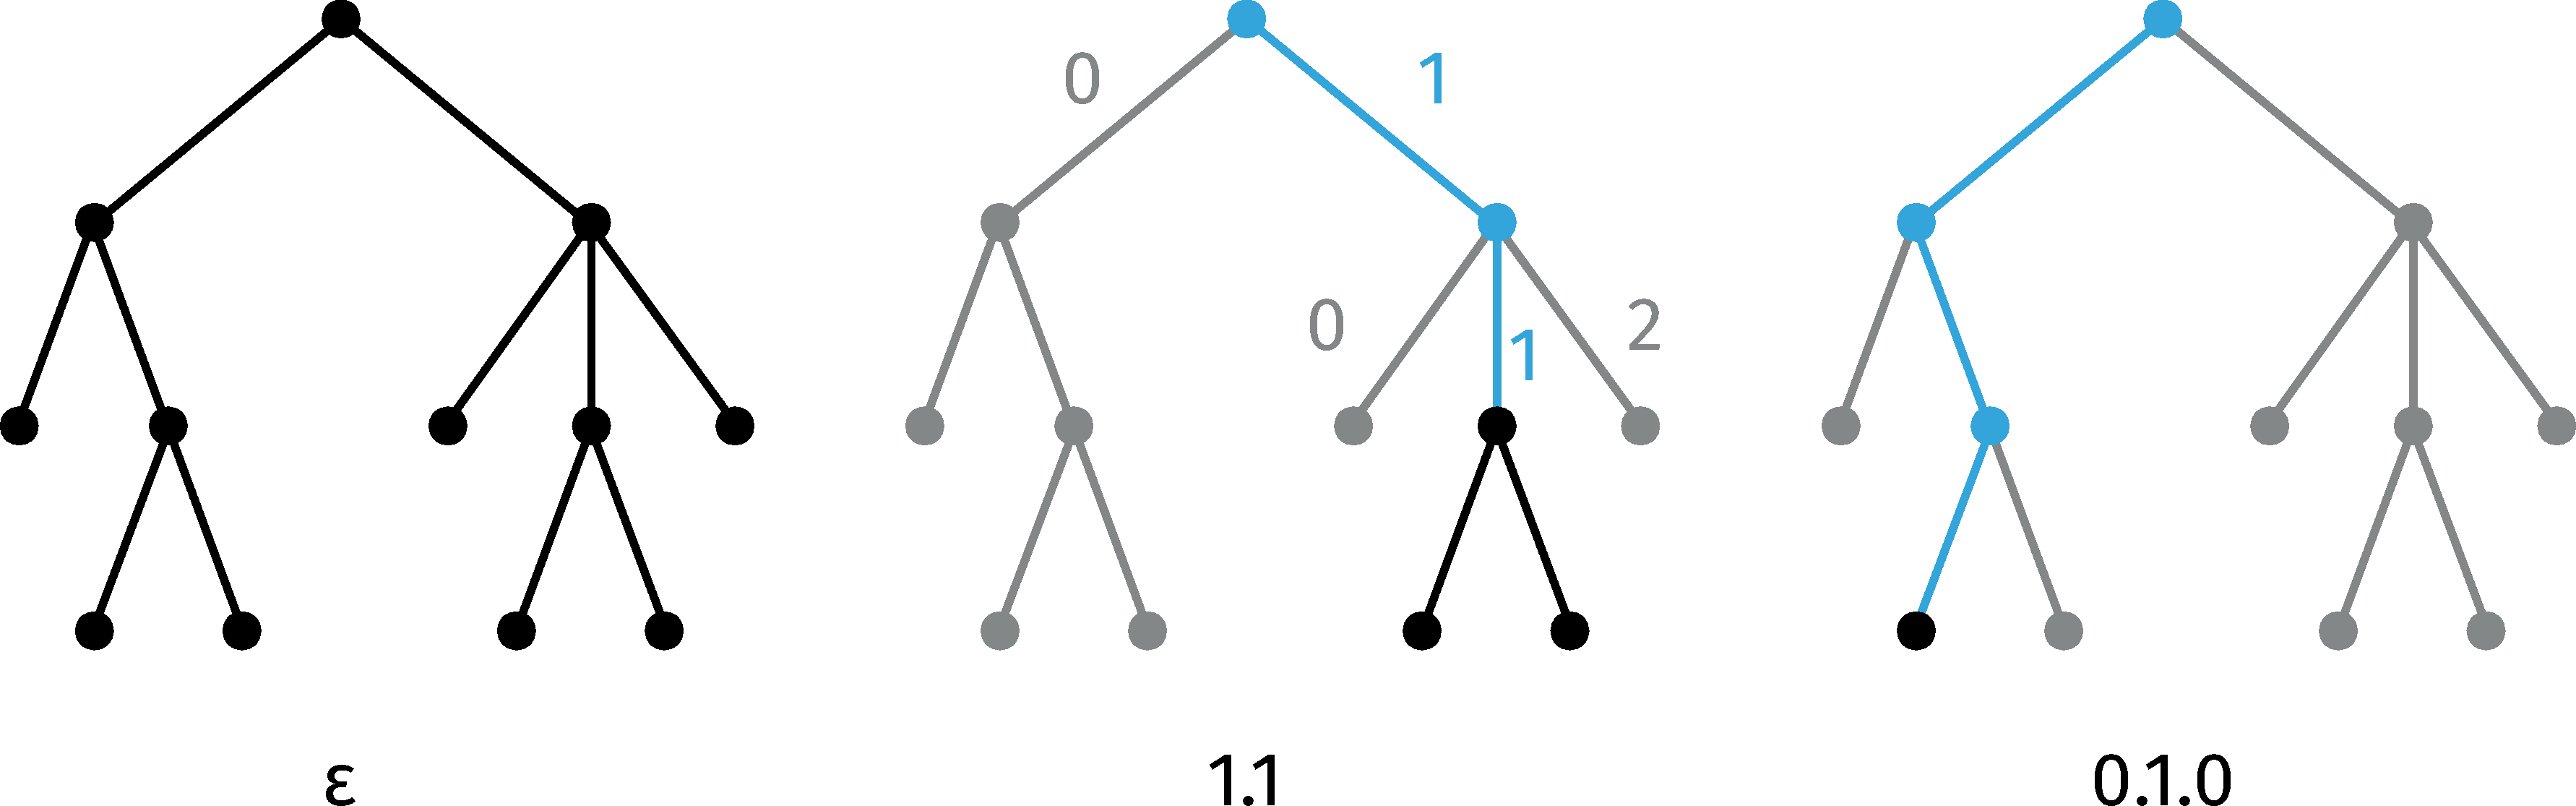
\includegraphics[width=0.9\textwidth]{tree-position.pdf}
\end{figure}

Now, terms are a special kind of tree so we can do something similar.
There are many ways to represent positions: for instance in the example above
the position \(0.3\) does not correspond to anything, so is it still considered
a position, only an \emph{invalid} one? Or should all expressable positions
be valid?

My approach is a bit in between, I constrain the syntax of choices a bit more
than this, but they are not necessarily valid.
Basically choices are defined inductively, with several constructors for each
of the constructs of the syntax: for instance, applications will have two
corresponding choices, one for the applicant, one for the argument.
\marginnote[1cm]{
  \mintinline{coq}{app_l} corresponds to going left under an application
  while \mintinline{coq}{app_r} corresponds to going right.
}
\begin{minted}{coq}
Inductive choice :=
| app_l
| app_r
| case_p
| case_c
| case_brs (n : nat)
| proj_c
| fix_mfix_ty (n : nat)
| fix_mfix_bd (n : nat)
| lam_ty
| lam_tm
| prod_l
| prod_r
| let_bd
| let_ty
| let_in.
\end{minted}

A position is just a list of choices.
\begin{minted}{coq}
Definition position := list choice.
\end{minted}

Now as I already said, these are not necessarily valid positions, for this
we define a function which verifies if a given position is valid in a given
term.
\marginnote[1cm]{
  It should not feel too surprising, the empty position is always valid,
  and otherwise, the head choice should match the structure of the term.
  There are some trickier cases for pattern-matching and fixed-points because
  they involve lists of terms but it is still pretty natural.
}
\begin{minted}{coq}
Fixpoint validpos t (p : position) {struct p} :=
  match p with
  | [] => true
  | c :: p =>
    match c, t with
    | app_l, tApp u v => validpos u p
    | app_r, tApp u v => validpos v p
    | case_p, tCase indn pr c brs => validpos pr p
    | case_c, tCase indn pr c brs => validpos c p
    | case_brs n, tCase indn pr c brs =>
        match nth_error brs n with
        | Some (_, br) => validpos br p
        | None => false
        end
    | proj_c, tProj pr c => validpos c p
    | fix_mfix_ty n, tFix mfix idx =>
        match nth_error mfix n with
        | Some d => validpos d.(dtype) p
        | None => false
        end
    | fix_mfix_bd n, tFix mfix idx =>
        match nth_error mfix n with
        | Some d => validpos d.(dbody) p
        | None => false
        end
    | lam_ty, tLambda na A t => validpos A p
    | lam_tm, tLambda na A t => validpos t p
    | prod_l, tProd na A B => validpos A p
    | prod_r, tProd na A B => validpos B p
    | let_bd, tLetIn na b B t => validpos b p
    | let_ty, tLetIn na b B t => validpos B p
    | let_in, tLetIn na b B t => validpos t p
    | _, _ => false
    end
  end.
\end{minted}
This function might serve as a specification for the positions.

Finally we can define a type of valid positions in a term using a subset type.
\begin{minted}{coq}
Definition pos (t : term) :=
  { p : position | validpos t p = true }.
\end{minted}

For instance \mintinline{coq}{[ app_l ; let_in ]} is valid position in term
\begin{minted}{coq}
  tApp (tLetIn na b B t) u
\end{minted}
which represents the term \mintinline{coq}{(let na := b : B in t) u}
and points to subterm \mintinline{coq}{t}.

We can also define a function to access the subterm at a given position.
\begin{minted}{coq}
Fixpoint atpos t (p : position) {struct p} : term :=
  match p with
  | [] => t
  | c :: p =>
    match c, t with
    | app_l, tApp u v => atpos u p
    | app_r, tApp u v => atpos v p
    | case_p, tCase indn pr c brs => atpos pr p
    | case_c, tCase indn pr c brs => atpos c p
    | case_brs n, tCase indn pr c brs =>
        match nth_error brs n with
        | Some (_, br) => atpos br p
        | None => tRel 0
        end
    | proj_c, tProj pr c => atpos c p
    | fix_mfix_ty n, tFix mfix idx =>
        match nth_error mfix n with
        | Some d => atpos d.(dtype) p
        | None => tRel 0
        end
    | fix_mfix_bd n, tFix mfix idx =>
        match nth_error mfix n with
        | Some d => atpos d.(dbody) p
        | None => tRel 0
        end
    | lam_ty, tLambda na A t => atpos A p
    | lam_tm, tLambda na A t => atpos t p
    | prod_l, tProd na A B => atpos A p
    | prod_r, tProd na A B => atpos B p
    | let_bd, tLetIn na b B t => atpos b p
    | let_ty, tLetIn na b B t => atpos B p
    | let_in, tLetIn na b B t => atpos t p
    | _, _ => tRel 0
    end
  end.
\end{minted}
\marginnote[-2.5cm]{
  The \mintinline{coq}{tRel 0} case is in an impossible branch when the position
  is valid, but for simplicity, the function is defined for any position.
  Otherwise we would have to carry the proof that it is valid everywhere.
}

Positions let you go deep inside a term, forgetting about its surrounding;
surrounding which can be recorded using stacks.

\section{Stacks}

My use of the term \emph{stack} might be an abuse as it is probably a
generalisation of it and might be better called an evaluation environment
or context; I will stick to \emph{stack} anyway.
The main reason behind the name is that it is not presented as a term with a hole
but rather as a succession of terms with a hole that stack on top of each other.

If you take the following example,
\[
  \stack{f\ \stack{\stack{(\lambda x. \stack{t})}\ u}}
\]
you are considering term \(t\) against the stack
\[
  \stack{f\ \stack{\stack{(\lambda x. \shole)}\ u}}
\]

It can be decomposed into
\marginnote[1cm]{
  \(\varepsilon\) represents the empty stack.
}
\[
  \stack{\lambda x. \shole} :: \stack{\shole\ u} :: \stack{f\ \shole}
  :: \varepsilon
\]
meaning that the term will first be put under an abstraction, the result of this
applied to \(u\) and the whole given as an argument to \(f\).
This notion will prove particularly useful when considering the reduction
machine in \nrefch{coq-reduction}, indeed the stack is way to remember the
surrounding term when focusing on a subterm, once it has reached a normal form,
we can use the stack as a \emph{continuation}.

You can see the process step by step in the following example.
\marginnote[2cm]{
  I use \(\red_\beta\) to denote the cases where a \emph{real} reduction
  happens and the focused term (a \(\lambda\)-abstraction) consumes its
  argument; the other cases are \emph{focusing}, \ie pushing some term with
  hole on the stack.
}
\[
  \begin{array}{lc}
    \stack{
      (
        (\lambda x.\ x\ u)\
        (\lambda y.\ y)
      ) \ v
    } & \red \\[0.2cm]
    \stack{
      \stack{(
        (\lambda x.\ x\ u)\
        (\lambda y.\ y)
      )} \ v
    } & \red \\[0.3cm]
    \stack{
      \stack{(
        \stack{(\lambda x.\ x\ u)}\
        (\lambda y.\ y)
      )} \ v
    } & \red_\beta \\[0.4cm]
    \stack{
      \stack{(
        (\lambda y.\ y)\ u
      )} \ v
    } & \red \\[0.3cm]
    \stack{
      \stack{(
        \stack{(\lambda y.\ y)}\ u
      )} \ v
    } & \red_\beta \\[0.4cm]
    \stack{
      \stack{u} \ v
    }
  \end{array}
\]

\marginnote{
  In the formalism above, \(\vscmd{t}{\stack{\shole\ u} :: \varepsilon}\)
  corresponds to \(\stack{\stack{t}\ u}\). I am simply now making explicit
  the separation between the focused term and the stack.
}
The intesting bit is that the focused term still interacts with the stack.
To see clearer we can use the notation \(\vscmd{t}{\pi}\) representing
term \(t\) \emph{against} stack \(\pi\). From this we can write the following
reduction rules that together correspond to \(\beta\)-reduction.

\marginnote[0.5cm]{
  \(\beta\)-reduction now happens in two steps:
  \(
    \vscmd{(\lambda x.\ t)\ u}{\pi} \red
    \vscmd{\lambda x.\ t}{\stack{\shole\ u} :: \pi} \red
    \vscmd{t[x \sto u]}{\pi}
  \)
}
\[
  \begin{array}{lcl}
    \vscmd{u \ v}{\pi} &\red& \vscmd{u}{\stack{\shole\ v} :: \pi} \\
    \vscmd{\lambda x.\ t}{\stack{\shole\ u} :: \pi}
    &\red& \vscmd{t[x \sto u]}{\pi}
  \end{array}
\]

In \Coq I define stacks as follows.
\begin{minted}{coq}
Inductive stack : Type :=
| Empty
| App (t : term) (π : stack)
| Fix (f : mfixpoint term) (n : nat) (args : list term)
      (π : stack)
| Fix_mfix_ty (na : name) (bo : term) (ra : nat)
              (mfix1 mfix2 : mfixpoint term) (id : nat)
              (π : stack)
| Fix_mfix_bd (na : name) (ty : term) (ra : nat)
              (mfix1 mfix2 : mfixpoint term) (id : nat)
              (π : stack)
| CoFix (f : mfixpoint term) (n : nat) (args : list term)
        (π : stack)
| Case_p (indn : inductive * nat) (c : term)
         (brs : list (nat * term)) (π : stack)
| Case (indn : inductive * nat) (p : term)
       (brs : list (nat * term)) (π : stack)
| Case_brs (indn : inductive * nat) (p c : term) (m : nat)
           (brs1 brs2 : list (nat * term)) (π : stack)
| Proj (p : projection) (π : stack)
| Prod_l (na : name) (B : term) (π : stack)
| Prod_r (na : name) (A : term) (π : stack)
| Lambda_ty (na : name) (b : term) (π : stack)
| Lambda_tm (na : name) (A : term) (π : stack)
| LetIn_bd (na : name) (B t : term) (π : stack)
| LetIn_ty (na : name) (b t : term) (π : stack)
| LetIn_in (na : name) (b B : term) (π : stack)
| coApp (t : term) (π : stack).

Notation "'ε'" := (Empty).
\end{minted}

\section{Positions induced by stacks}

The reason I present stacks and positions together is because they are related.
If you consider the term \(t\) against some stack \(\pi\) as one term, there
exists a position in that term that points to \(t\).
For instance if you consider
\[
  \stack{u\ \stack{\stack{t}\ v}}
\]
then the position that first chooses the right-hand term of the top-level
application and then the left-hand term will indeed point to \(t\).
In \Coq syntax as earlier this would be
\begin{minted}{coq}
[ app_r ; app_l ]
\end{minted}

In fact the position can be computed from the stack itself, regardless of the
term we want to plug in. In the example above, the stack is
\[
  \stack{\shole\ v} :: \stack{u\ \shole} :: \varepsilon
\]
We read it from right to left\sidenote{This is because the leftmost term with
hole corresponds to the innermost element in the resulting term.} to reconstruct
the position and simply give the position of the hole.

\begin{minted}{coq}
Fixpoint stack_position π : position :=
  match π with
  | ε => []
  | App u ρ => stack_position ρ ++ [ app_l ]
  | Fix f n args ρ => stack_position ρ ++ [ app_r ]
  | Fix_mfix_ty na bo ra mfix1 mfix2 idx ρ =>
      stack_position ρ ++ [ fix_mfix_ty #|mfix1| ]
  | Fix_mfix_bd na ty ra mfix1 mfix2 idx ρ =>
      stack_position ρ ++ [ fix_mfix_bd #|mfix1| ]
  | CoFix f n args ρ => stack_position ρ ++ [ app_r ]
  | Case_p indn c brs ρ => stack_position ρ ++ [ case_p ]
  | Case indn pred brs ρ => stack_position ρ ++ [ case_c ]
  | Case_brs indn pred c m brs1 brs2 ρ =>
      stack_position ρ ++ [ case_brs #|brs1| ]
  | Proj pr ρ => stack_position ρ ++ [ proj_c ]
  | Prod_l na B ρ => stack_position ρ ++ [ prod_l ]
  | Prod_r na A ρ => stack_position ρ ++ [ prod_r ]
  | Lambda_ty na u ρ => stack_position ρ ++ [ lam_ty ]
  | Lambda_tm na A ρ => stack_position ρ ++ [ lam_tm ]
  | LetIn_bd na B u ρ => stack_position ρ ++ [ let_bd ]
  | LetIn_ty na b u ρ => stack_position ρ ++ [ let_ty ]
  | LetIn_in na b B ρ => stack_position ρ ++ [ let_in ]
  | coApp u ρ => stack_position ρ ++ [ app_r ]
  end.
\end{minted}

As I said multiple times, we will use stacks for reduction machines, to show the
termination of such machines it is nice to have an order on stacks. This order
will be achieved by going from stacks to positions.

\section{Ordering positions}

If you consider the valid positions in a given term (\ie expressions of type
\mintinline{coq}{pos t} for some \mintinline{coq}{t}) there exists a
well-founded order on them. There are actually several due to some degree of
liberty as we shall see.

Since positions are defined as lists, the natural order on them would the
structural which says that any (strict) prefix of a position is smaller.
This order is not really of interest to us because it would correspond to
\emph{unfocusing}.
Conversely, by extending a position with a new choice you are going deeper into
the term, something which you cannot do indefinitely, you are bound to reach a
leaf at some (finite) point.

If you think about it dually, I'm merely explaining that the structural order on
terms is well-founded, so why bother?
The interesting part is that the order on positions can be more flexible than
the subterm relation in that it allows us to compare `going left' with
`going right'.
Say you have the application \(t \coloneqq u\ v\), both \(u\) and \(v\) are
subterms of \(t\) but there is no way to relate the two of them reliably and
have \(v\) \emph{always} smaller than \(u\) because \(u\) and \(v\) can be
arbitrary.
If instead we were to consider positions in \(t\) we would have the empty one
corresponding to \(t\) itself, \mintinline{coq}{[ app_l ]} corresponding to
\(u\) and \mintinline{coq}{[ app_r ]} for \(v\). This means we abstract over the
content of both \(u\) and \(v\). The positions can thus be ordered as follows:
\begin{minted}{coq}
[ app_r ] < [ app_l ] < []
\end{minted}

I am going to explain why this is desirable in \nrefch{coq-reduction}.

In \Coq, the definition of the order is done in two steps: first an order on
raw positions, from which we then derive an order on valid positions.
\marginnote[4.8cm]{
  The \mintinline{coq}{(` p)} notation corresponds to the first projection of
  a subset type.
}
\begin{minted}{coq}
Inductive positionR : position -> position -> Prop :=
| positionR_app_lr p q :
    positionR (app_r :: p) (app_l :: q)

| positionR_deep c p q :
    positionR p q ->
    positionR (c :: p) (c :: q)

| positionR_root c p :
    positionR (c :: p) [].

Definition posR {t} (p q : pos t) : Prop :=
  positionR (` p) (` q).
\end{minted}

While the first order is not well-founded, the second one is, as crystallised
by the following lemma.
\begin{minted}{coq}
Lemma posR_Acc :
  forall t p, Acc (@posR t) p.
\end{minted}
% \setchapterpreamble[u]{\margintoc}
\chapter{Reduction}
\labch{coq-reduction}

A key element to defining a type checker is to have a conversion checker.
Conversion in turn relies on reduction. The reduction I describe in
\nrefch{coq-spec} is just a relation and is non-deterministic. In this chapter
I will present an algorithmic implementation of reduction.
This implementation relies on the axiom of strong normalisation, but even then
it requires some more work to show the process is terminating.

\section{Weak head normalisation}

Since reduction is non deterministic, we have to pick a strategy to implement.
When checking terms for conversion, one thing we want to do is verify that they
have the same head constructor: if two terms are \(\lambda\)-abstractions
\(\lambda (x:A).t\) and \(\lambda (x:A').t'\) we need only compare \(A\) and
\(A'\), as well as \(t\) and \(t'\) for conversion.
Weak head reduction is a strategy that allows us to access the head of a term
rather efficiently.

The idea is to only deal with redexes (\ie left-hand side of reduction rules)
that appear at the top-level and might be hiding the head constructor. As such
when considering \(\lambda (x:A).t\), neither \(A\) nor \(t\) will be reduced
because we already know the head, or the shape, of the term: it is a
\(\lambda\). However, if we have an application \(t\ u\), we will first weak
head reduce \(t\) to see if it reaches a \(\lambda\): if it does we substitute
\(u\) and repeat the process, if it does not, then we have reached a weak head
normal form.

Weak head normal forms are by definition the terms that cannot be reduced
further by weak head reduction.

\begin{definition}[Normal form]
  A term \(t\) is a normal form for a reduction \(\red\) if it doesn't reduce
  for \(\red\).
  \[
    t \not \red
  \]
\end{definition}

It is however possible to characterise weak
head normal forms syntactically. For this we need to talk about \emph{neutral}
forms.

\begin{definition}[Neutral forms]
  A term \(t\) is neutral for a reduction \(\red\) if substituting it inside
  another term doesn't introduce redexes. Equivalently substituting a neutral
  term \(t\) in a normal form \(u\) will yield another normal form.
  \[
    u[x \sto t] \not \red
  \]
\end{definition}

\todo{Syntactic characterisation, on simple case and/or code version?}
% \setchapterpreamble[u]{\margintoc}
\chapter{Conversion}
\labch{coq-conversion}

We want to implement a correct conversion checker that is close enough to the
actual implementation that is rather efficient, instead of the naive solution
of reducing both terms to normal forms and then comparing them syntactically.
We also have to take care of universes and cumulativity which complicates matter
a little bit.

\section{High level description}

I will present our approach at the high level.
\begin{enumerate}[label=(\arabic*)]
  \item \label{itm:convred} First we weak head reduce the two terms without
  \(\delta\)-reduction (\ie without unfolding definitions);
  \item then we compare their heads, if they match we begin again at
  \ref{itm:convred};
  \item if they do not match, we check if some computation (pattern-matching
  or fixed-point)---or even the whole term---is blocked by a definition that
  could unfold to a value, and if so we unfold the definition and start again.
\end{enumerate}

Following reduction, we actually use terms versus stacks to deal with focusing.
Conversion is in fact split in four main phases that I codify as follows
\begin{itemize}
  \item \mintinline{coq}{Reduction} which corresponds to putting the two terms
  in weak head normal forms;
  \item \mintinline{coq}{Term} which corresponds to comparing the heads of the
  focused terms;
  \item \mintinline{coq}{Args} which corresponds to comparing the arguments
  on the stacks;
  \item \mintinline{coq}{Fallback} which happens when comparing different heads
  and we attempt to reduce both sides a bit more.
\end{itemize}
These roughly correspond each to one of the mutual definitions that yield
conversion. I will write these functions as judgements:
\marginnote[0.5cm]{
  Here I forget about the typing requirements, but conversion, like reduction,
  can only operate on well-typed terms.
}
\[
  \begin{array}{c}
    \isconv{\Ga}{t_1}{\pi_1}{t_2}{\pi_2}{A}
  \end{array}
\]
where \(A\) is the \emph{answer} which is basically `yes' or an error message.
\(A\) is the \emph{output} while everything else is the \emph{input}.
I will use the subscripts \(\cred\), \(\cterm\), \(\cargs\) and \(\cfall\)
to diffrenciate the four phases.
I will present them in more depth so that we can see what are
the requirements for termination.

\subsection{\mintinline{coq}{Reduction}}

The first phase takes two pairs of term and stack and reduce both using the
weak head reduction machine of \nrefch{coq-reduction}.
In order to avoid unfolding definitions unnecessarily, we disable the
\(\delta\)-reduction.
% This means that we pass the
% \begin{minted}{coq}
% RedFlags.nodelta
% \end{minted}
% flags to the machine.
This means that we pass the \mintinline{coq}{RedFlags.nodelta} flags to the
machine.

I will once again describe these functions and their recursive calls using
inference rules for simplicity.
\begin{mathpar}
  \infer
    {
      \Ga \vdash \vscmd{t_1}{\pi_1} \red_{\WM \not\delta} \vscmd{u_1}{\rho_1} \\
      \Ga \vdash \vscmd{t_2}{\pi_2} \red_{\WM \not\delta} \vscmd{u_2}{\rho_2} \\
      \convterm{\Ga}{u_1}{\rho_1}{u_2}{\rho_2}{A}
    }
    {\convred{\Ga}{t_1}{\pi_1}{t_2}{\pi_2}{A}}
  %
\end{mathpar}
Here we simply do a recursive call on the weak head normal forms of the two
inputs.

\subsection{\mintinline{coq}{Term}}

For this phase, we take two inputs that are in weak head normal form (without
\(\delta\)-reduction) and look at the heads of the terms.
The idea behind disabling \(\delta\) is that when comparing two constants
we hope not to have to unfold them if they already are the same.
\[
  \infer
    {
      u_1 \cong u_2 \\
      \convargs{\Ga}{\const\ k\ u_1}{\pi_1}{\const\ k\ u_2}{\pi_2}{\ayes}
    }
    {\convterm{\Ga}{\const\ k\ u_1}{\pi_1}{\const\ k\ u_2}{\pi_2}{\ayes}}
  %
\]
where \(\const\ k\ u\) refers to the constant of name \(k\) and universe
instance \(u\).
Here we first compare the universe instances to check that they are equal
(which is a bit more general that syntactic equality), and if so we compare
the stacks, or more specifically the arguments on those. I will explain this
part when presenting the corresponding function.
\marginnote[0.1cm]{
  One or the two of them might refer to axioms and in that case, we only unfold
  those that can be, and if we compare two axioms, we know they are distinct.
}
If the constant names aren't the same, or if the universe instances do not match
or if the argument comparison fails, we then unfold one of the constants and
compare them again.
\marginnote[1cm]{
  I informally write \(t_2[u_2]\) to mean \(t_2\) instantiated by \(u_2\).
}
\[
  \infer
    {
      (k_2 := t_2) \in \Sigma \\
      \convred{\Ga}{\const\ k_1\ u_1}{\pi_1}{t_2[u_2]}{\pi_2}{A}
    }
    {\convterm{\Ga}{\const\ k_1\ u_1}{\pi_1}{\const\ k_2\ u_2}{\pi_2}{A}}
  %
\]

Another interesting case is the comparison of \(\lambda\)-abstractions.
\marginnote[1cm]{
  Once again I show the rule when there are successes in each recursive calls,
  all the others yield errors.
}
\[
  \infer
    {
      \convred
        {\Ga}
        {A_1}
        {\stack{\lambda (x:\shole).\ t_1} :: \pi_1}
        {A_2}
        {\stack{\lambda (x:\shole).\ t_2} :: \pi_2}
        {\ayes}
      \\
      \convred
        {\Ga}
        {t_1}
        {\stack{\lambda (x:A_1).\ \shole} :: \pi_1}
        {t_2}
        {\stack{\lambda (x:A_2).\ \shole} :: \pi_2}
        {A}
    }
    {
      \convterm
        {\Ga}
        {\lambda (x:A_1).\ t_1}{\pi_1}
        {\lambda (x:A_2).\ t_2}{\pi_2}
        {A}
    }
  %
\]
First we compare the two domains and then we compare the two bodies.
This may seem like a simple case of recursing in the subterms but there is a
subtlety: the context when comparing the bodies is still \(\Ga\) and not
\(\Ga, x:A_1\) or \(\Ga, x:A_2\).
\marginnote[0.1cm]{
  A \emph{good} things that helps us complete proofs.
}
This is actually a good thing that we don't have to pick one of them and remain
symmetric.
We are saved by the stacks once more. Indeed, in
\(\stack{\lambda (x:A_1).\ \shole}\) we have the information corresponding to
\(x : A_1\). More generally, stacks do not only yield positions but also
contexts. In the expression
\[
  \isconv{\Ga}{t_1}{\pi_1}{t_2}{\pi_2}{A}
\]
\(t_1\) lives in \(\Ga, \stackctx\ \pi_1\), and \(t_2\) in
\(\Ga, \stackctx\ \pi_2\).

Other than those, we also deal with \(\Pi\)-types, pattern-matching,
projections, fixed- and cofixed-points.
The case of two applications is imposibble because the arguments would have been
pushed on the stacks.
If the terms do not fall in this diagonal, we instead call the fallback
function recursively.
\[
  \infer
    {\convfall{\Ga}{t_1}{\pi_1}{t_2}{\pi_2}{A}}
    {\convterm{\Ga}{t_1}{\pi_1}{t_2}{\pi_2}{A}}
  %
\]

\subsection{\mintinline{coq}{Args}}

When the two terms are convertible, it is time to move on the comparison of the
stacks, or rather the comparision of the leading arguments on said stacks.

A stack \(\pi\) can be decomposed into a list of arguments \(u_1, \dots, u_n\)
and a remaining stack \(\rho\) that does not start with some \(\coapp{u}\),
such that
\[
  \pi = \coapp{u_1} :: \dots :: \coapp{u_n} :: \rho
\]
With two such decomposed stacks, the meaning of the \mintinline{coq}{Args}
function is the following
\marginnote[1cm]{
  Notice how we have \(n\) arguments on both sides, if there is a mismatch,
  the function will return an error.
}
\[
  \footnotesize
  \infer
    {
      \convred
        {\Ga}
        {u_1}
        {\stack{t_1\ \shole\ u_2\ \dots u_n} :: \rho_1}
        {v_1}
        {\stack{t_2\ \shole\ v_2\ \dots v_n} :: \rho_2}
        {\ayes}
      \\\\
      \vdots \\\\
      \convred
        {\Ga}
        {u_n}
        {\stack{t_1\ u_1\ \dots u_{n-1}\ \shole} :: \rho_1}
        {v_n}
        {\stack{t_2\ v_1\ \dots v_{n-1}\ \shole} :: \rho_2}
        {\ayes}
    }
    {
      \convargs
        {\Ga}
        {t_1}
        {\coapp{u_1} :: \dots :: \coapp{u_n} :: \rho_1}
        {t_2}
        {\coapp{v_1} :: \dots :: \coapp{v_n} :: \rho_2}
        {A}
    }
  %
\]
Assuming that \(\Ga \vdash u_1 \equiv u_2\), it saying `yes' means that
\[
  \Ga \vdash t_1\ u_1\ \dots\ u_n \equiv t_2\ v_1\ \dots\ v_n
\]
(and also the stronger property that each \(u_i\) is convertible to \(v_i\) but
the property above is sufficient for our needs).

\subsection{\mintinline{coq}{Fallback}}

The fallback deals with terms outside of the diagonal that are potentially
stuck because of definitions that are not unfolded.
It tries to make progress on each side before resorting to plain and simple
syntactic equality.
\marginnote[1cm]{
  I use \(\red_\WM \not =\) to mean that the reduction produced a different term.
  In the formalisation its a different process that checks that the term is
  indeed stuck because of \(\delta\).
}
\marginnote[4.4cm]{
  Here \(t_1 = t_2\) means that \(t_1\) and \(t_2\) have been checked to be
  syntactically equal, up to universes.
}
\begin{mathpar}
  \infer
    {
      \Ga \vdash \vscmd{t_1}{\pi_1} \red_\WM \not= \vscmd{u}{\rho} \\
      \convterm{\Ga}{u}{\rho}{t_2}{\pi_2}{A}
    }
    {\convfall{\Ga}{t_1}{\pi_1}{t_2}{\pi_2}{A}}
  %

  \infer
    {
      \Ga \vdash \vscmd{t_2}{\pi_2} \red_\WM \not= \vscmd{u}{\rho} \\
      \convterm{\Ga}{t_1}{\pi_1}{u}{\rho}{A}
    }
    {\convfall{\Ga}{t_1}{\pi_1}{t_2}{\pi_2}{A}}
  %

  \infer
    {
      t_1 = t_2 \\
      \convargs{\Ga}{t_1}{\pi_1}{t_2}{\pi_2}{A}
    }
    {\convfall{\Ga}{t_1}{\pi_1}{t_2}{\pi_2}{A}}
  %
\end{mathpar}

\subsection{About cumulativity and universes}

In the (partial) definitions above I sometimes refer to syntactic equality of
terms or equality of universes. These are alaways refering to the universe
constraints to be decided, \ie their respective representations need not be the
same on both sides of the equality. This is the reason why I write \(u = v\)
when I could have unified them, the way I unified \(k_1\) and \(k_2\) into \(k\)
when considering constants.

Another important point is that we actually define conversion and cumulativity
at the same time, using an extra argument (essentially a boolean) telling us
which of those we are checking for.
I did everything in the setting of conversion to have lighter notations, but
everything works just as well with cumulativity.

I will not explain how we specify and check equality or cumulativity of
universes as it was not my own contribution.
The interested reader should refer either to~\sidecite{sozeau2019coq} or the
formalisation.

\section{Termination and correctness}

\subsection{Specification}

You will perhaps find my presentation surprising in that I didn't even specify
what was expected of the algorithm I was showing. I wanted to focus on the
intuition before going into these details.
It is time to correct this slight.

All the `judgements' I presented earlier, that is
\[
  \begin{array}{l}
    \convred{\Ga}{t_1}{\pi_1}{t_2}{\pi_2}{A} \\
    \convterm{\Ga}{t_1}{\pi_1}{t_2}{\pi_2}{A} \\
    \convargs{\Ga}{t_1}{\pi_1}{t_2}{\pi_2}{A} \\
    \convfall{\Ga}{t_1}{\pi_1}{t_2}{\pi_2}{A}
  \end{array}
\]
are correct if, when they return \(\ayes\), we have
\[
  \Ga \vdash t_1\ u_1\ \dots\ u_n \equiv t_2\ v_1\ \dots\ v_n
\]
where \(\pi_1\) and \(\pi_2\) are decomposed as
\[
  \begin{array}{rcl}
    \pi_1 &=& \coapp{u_1} :: \dots :: \coapp{u_n} :: \rho_1 \\
    \pi_2 &=& \coapp{v_1} :: \dots :: \coapp{v_n} :: \rho_2
  \end{array}
\]
This might be a bit surprising that we only conclude on applications at the head
of the stakcs and not about the whole stacks themselves.
If we were asking for
\[
  \Ga \vdash \zip\ \vscmd{t_1}{\pi_1} \equiv \vscmd{t_2}{\pi_2}
\]
instead, it would be too strong a requirement. Indeed, in the case of
\(\lambda\)-abstractions, we consider the recrusive call on the domains
\marginnote[1cm]{
  Note that \(\zip\ \vscmd{A}{\stack{\lambda (x:\shole).t} :: \pi}\)
  is equal to \(\zip\ \vscmd{\lambda (x:A).t}{\pi}\).
}
\[
  \convred
    {\Ga}
    {A_1}
    {\stack{\lambda (x:\shole).\ t_1} :: \pi_1}
    {A_2}
    {\stack{\lambda (x:\shole).\ t_2} :: \pi_2}
    {\ayes}
\]
which we want to conclude on \(A_1\) and \(A_2\), not on the full term,
otherwise the recusrive call on the bodies becomes superfluous.
This, I think, is a sign, that this approach is doomed to fail.

Going back to the bigger picture, it is also not a problem that we conclude only
on a portion of the stack since the conversion algorithm will be called with
empty stacks at the start.
\marginnote[0.8cm]{
  As you can see we also call the \mintinline{coq}{Reduction} phase first as
  well.
}
\[
  \convred{\Ga}{t_1}{\varepsilon}{t_2}{\varepsilon}{A}
\]

We can now move on to the main difficulty regarding conversion: its termination.

\subsection{Termination}

You can see that the definition of the conversion algorithm is reminiscent of
that of weak head reduction, and one might expect the termination orders to be
relatively close. This is indeed the case, but things are slightly more
complicated here, mainly for two reasons: we sometimes consider terms up to
universes; and we have mutually defined functions.

I will go over the different kind of recursive calls to motivate the order,
before introducing it.

The first rule I presented involves putting both terms in weak head normal
form before recursing on them. As we know from the correctness of weak head
reduction, the terms it yields are reducts of the orginal terms, and some
focusing potentially happened. As such, the order used by reduction seems like
a good option, save for one problem: in some cases---when the term is already
in weak head normal form---the weak reduction returns the original term.
Because of this, the phases must be part of the order.
In particular we want to have
\[
  \cterm \prec \cred
\]

Similarly, when comparing constants in the \mintinline{coq}{Term} phase,
we have a recursive call to the \mintinline{coq}{Args} phase with the same
arguments so we also want
\[
  \cargs \prec \cterm
\]
When we unfold one of the constants however, we go back from the
\mintinline{coq}{Term} phase to the \mintinline{coq}{Reduction} phase
so we really have to account for the fact that the unfolded definition is a
reduct of the constant, and it has to come before in the lexicographical
order.

The case of \(\lambda\)-abstractions tells us that similarly, the subterm
relation should come before the phase relation.

The \mintinline{coq}{Fallback} phase also happens with the same arguments as
that of the \mintinline{coq}{Term} phase so
\[
  \cfall \prec \cterm
\]

The \mintinline{coq}{Args} phase makes recrusive calls inside the stack meaning
that, like weak head reduction, we must in fact use positions rather than the
subterm relation.

Finally, the \mintinline{coq}{Fallback} phase can make recursive calls on the
\mintinline{coq}{Args} phase with the same arguments, meaning
\[
  \cargs \prec \cfall
\]

\paradot{The order}

Let me now introduce the order that we use to prove conversion terminating.
First we need to define the notion of phases (that I call states in the
formalisation):
\begin{minted}{coq}
Inductive state :=
| Reduction
| Term
| Args
| Fallback.
\end{minted}
as well as a well-founded order on them
\marginnote[0.3cm]{
  It should not prove to hard to see that it is indeed well-founded since we
  essentially have
  \[
    \cargs \prec \cfall \prec \cterm \prec \cred
  \]
}
\begin{minted}{coq}
Inductive stateR : state -> state -> Prop :=
| stateR_Term_Reduction : stateR Term     Reduction
| stateR_Args_Term      : stateR Args     Term
| stateR_Fallback_Term  : stateR Fallback Term
| stateR_Args_Fallback  : stateR Args     Fallback.
\end{minted}

I already said we needed to consider equality of terms up to universes, as such
we define an altered version of coreduction that is coreduction up to universes.
\marginnote[0.6cm]{
  The notation \mintinline{coq}{∥ A ∥} is for the \emph{squashed} version of
  \mintinline{coq}{A}, \ie its plunging into \mintinline{coq}{Prop}.
  This is to make sure it goes away after extraction.
}
\begin{minted}{coq}
Notation eqt u v :=
  (∥ eq_term (global_ext_constraints Σ) u v ∥).

Definition cored' Γ u v :=
  exists u' v', cored Σ Γ u' v' /\ eqt u u' /\ eqt v v'.
\end{minted}

\marginnote[2cm]{
  \mintinline{coq}{` w} is the first projection of \mintinline{coq}{w}, \ie
  a term, forgetting about its well-formedness proof.
}
Because coreduction is only well-founded for well-formed terms, I also define
the type of well-formed terms and coreduction on them.
\begin{minted}{coq}
Definition wterm Γ :=
  { t : term | wellformed Σ Γ t }.

Definition wcored Γ (u v : wterm Γ) :=
  cored' Σ Γ (` u) (` v).

Definition weqt {Γ} (u v : wterm Γ) :=
  eqt (` u) (` v).
\end{minted}

We can finally move on to the definition of the (auxiliary) order:
\marginnote[0.6cm]{
  Here I use \Equations which allows me to leave the coercions blank and provide
  them using tactics.
}
\begin{minted}{coq}
Equations R_aux (Γ : context) :
  (∑ t : term, pos t × (∑ w : wterm Γ, pos (` w) × state)) ->
  (∑ t : term, pos t × (∑ w : wterm Γ, pos (` w) × state)) ->
  Prop :=
  R_aux Γ :=
    t ⊨ eqt \ cored' Σ Γ by _ ⨷
    @posR t ⊗
    w ⊨ weqt \ wcored Γ by _ ⨷
    @posR (` w) ⊗
    stateR.
\end{minted}
So what we have here are nested dependent lexicographical orders modulo
syntactical equality up to universes.
The order operates on a term, a position in it, another term and position, and
finally a state, using coreduction for terms.

The real order simply repacks this information, computing the positions from
the stacks.
\begin{minted}{coq}
Record pack (Γ : context) := mkpack {
  st   : state ;
  tm1  : term ;
  stk1 : stack ;
  tm2  : term ;
  stk2 : stack ;
  wth  : wtp Γ tm2 stk2
}.

Arguments st {_} _.
Arguments tm1 {_} _.
Arguments stk1 {_} _.
Arguments tm2 {_} _.
Arguments stk2 {_} _.
Arguments wth {_} _.

Notation pzt u := (zipc (tm1 u) (stk1 u)) (only parsing).
Notation pps1 u := (stack_pos (tm1 u) (stk1 u)) (only parsing).
Notation pwt u := (exist _ (wth u)) (only parsing).
Notation pps2 u := (stack_pos (tm2 u) (stk2 u)) (only parsing).

Notation obpack u :=
  (pzt u ; (pps1 u, (pwt u ; (pps2 u, st u)))) (only parsing).

Definition R Γ (u v : pack Γ) :=
  R_aux Γ (obpack u) (obpack v).
\end{minted}

The order is well-founded and sufficient to prove termination of the conversion
algorithm which is also correct by construction.
In the end we get a conversion checker that operates on well-formed terms and
is proven sound:
\begin{minted}{coq}
Theorem isconv_term_sound :
  forall Γ leq t1 h1 t2 h2,
    isconv_term Γ leq t1 h1 t2 h2 = Success I ->
    conv_cum leq Σ Γ t1 t2.
\end{minted}
where \mintinline{coq}{leq} is the flag saying whether we compare for
cumulativity or conversion, and \mintinline{coq}{conv_cum leq} is either
cumulativity or conversion.

\section{Future work: \(\eta\)-conversion}

In the \Coq implementation, \(\eta\)-expansion is handled even though the
conversion is untyped. The way this is achieved is by only expanding a term
(which is not a \(\lambda\)-abstraction) when it is compared to a
\(\lambda\)-abstraction.
\[
  \infer
    {\convterm{\Ga}{\lambda (x:A).\ t_1\ x}{\pi_1}{\lambda (x:A).\ u}{\pi_2}{A}}
    {\convterm{\Ga}{t_1}{\pi_1}{\lambda (x:A).\ u}{\pi_2}{A}}
  %
\]
The recursive call would thus be followed by the congruence rule for
\(\lambda\)-abstractions.
For termination purposes this step is actually skipped and we directly do
\marginnote[1cm]{
  We also take advantage of this to skip the comparison of the domains since
  they are both necessarily the same.
}
\[
  \infer
    {
      \convred
        {\Ga}
        {t_1\ x}
        {\stack{\lambda (x:A).\ \shole} :: \pi_1}
        {u}
        {\stack{\lambda (x:A).\ \shole} :: \pi_2}
        {A}
    }
    {\convterm{\Ga}{t_1}{\pi_1}{\lambda (x:A).\ u}{\pi_2}{A}}
  %
\]

In our setting however, we would need to have the order not only modulo
universes but also modulo \(\eta\), and I have not yet managed to find a way
to account for \(\eta\) in a way that preserves well-foundedness.
As unfortunate as it is---it gets in the way of actually using our typechecker
on real-life examples---it will have to be future work for us.
% \setchapterpreamble[u]{\margintoc}
\chapter{Type inference and checking}
\labch{coq-inference}

Now that we have our conversion algorithm, we can move on to type-checking.
This work is not mine but that of Simon Boulier so I will go over it briefly.
It needs to be mentioned as it is the goal of both the weak head reduction
and the conversion algorithms.

\paradot{Inference versus checking}
In \Coq, without existential variables, type inference is decidable. That is,
given a term of \acrshort{PCUIC} in a well-formed environment \(\Ga\), there is
an algorithm that decides whether there exists a type \(A\) such that
\[
  \Ga \vdash t : A
\]
\marginnote[-0.3cm]{
  This implies that the inference algorithm should not return any type, but the
  principal type of \(t\).
}%
Checking that \(t\) has type \(B\) is then implemented by inferring the type of
\(A\) and verifying that it is a subtype of \(B\).

The good news is that this time, termination is structural so it does not require
extra work like we had for reduction and conversion.
Inference looks like this
\begin{minted}{coq}
Program Fixpoint infer
  (Γ : context) (HΓ : ∥ wf_local Σ Γ ∥) (t : term) {struct t}
  : typing_result ({ A : term & ∥ Σ ;;; Γ |- t : A ∥ }) :=
  match t with
  | tRel n =>
    match nth_error Γ n with
    | Some c => ret ((lift0 (S n)) (decl_type c) ; _)
    | None   => raise (UnboundRel n)
    end

  | tSort u =>
    match Universe.get_is_level u with
    | Some l =>
      check_eq_true
        (LevelSet.mem l (global_ext_levels Σ))
        (Msg ("undeclared level " ++ string_of_level l)) ;;
      ret (tSort (Universe.super l) ; _)
    | None  =>
      raise (Msg (string_of_sort u ++ " is not a level"))
    end

  | tProd na A B =>
    s1 <- infer_type infer Γ HΓ A ;;
    s2 <- infer_type infer (Γ ,, vass na A) _ B ;;
    ret (tSort (Universe.sort_of_product s1.π1 s2.π1) ; _)

  | tLambda na A t =>
    s1 <- infer_type infer Γ HΓ A ;;
    B <- infer (Γ ,, vass na A) _ t ;;
    ret (tProd na A B.π1 ; _)

  | tLetIn n b b_ty b' =>
    infer_type infer Γ HΓ b_ty ;;
    infer_cumul infer Γ HΓ b b_ty _ ;;
    b'_ty <- infer (Γ ,, vdef n b b_ty) _ b' ;;
    ret (tLetIn n b b_ty b'_ty.π1 ; _)

  | tApp t u =>
    ty <- infer Γ HΓ t ;;
    pi <- reduce_to_prod Γ ty.π1 _ ;;
    infer_cumul infer Γ HΓ u pi.π2.π1 _ ;;
    ret (subst10 u pi.π2.π2.π1 ; _)

  | tConst cst u =>
    match lookup_env (fst Σ) cst with
    | Some (ConstantDecl d) =>
      check_consistent_instance d.(cst_universes) u ;;
      let ty := subst_instance_constr u d.(cst_type) in
      ret (ty ; _)
    |  _ => raise (UndeclaredConstant cst)
    end

  (* ... *)

  end.
\end{minted}

We use \Program this time to allow us to solve some parts using tactics as,
once again, the function is defined to be correct by construction.
The function is written in monadic style, using the following monad
\begin{minted}{coq}
Inductive typing_result (A : Type) :=
| Checked (a : A)
| TypeError (t : type_error).
\end{minted}
which corresponds to either returning a type or an error message.

We can then decide checking
\begin{minted}{coq}
Program Definition infer_cumul Γ HΓ t A (hA : wellformed Σ Γ A)
  : typing_result (∥ Σ ;;; Γ |- t : A ∥) :=
  A' <- infer Γ HΓ t ;;
  X <- convert_leq Γ A'.π1 A _ _ ;;
  ret _.
\end{minted}

I do not expect you to read the definition in detail. For a variable it checks if
it is bound, and if so returns the type it is assigned in the environment,
otherwise it raises an error.
For a sort, it checks if it is algebraic, if not and it is a declared level,
it returns the successor level.
For a \(\Pi\)-type it infers the types of the domain and codomain, checking that
they are indeed sorts, and returns the sort of the product (\ie the maximum
of the two sorts if the second one is not \(\Prop\), and \(\Prop\) otherwise).
In the case of application we use \mintinline{coq}{infer_cumul} to \emph{check}
rather than infer the type of the argument. The checking function is defined
afterwards so this is another version of it (as you can see it takes
\mintinline{coq}{infer} as argument).

All this is as one should expect, and concludes our quest of a type-checker
defined in \Coq and proven correct while relying only on a few axioms stating
that the theory is well behaved.
% \setchapterpreamble[u]{\margintoc}
\chapter{Towards completeness}
\labch{coq-completeness}
% \setchapterpreamble[u]{\margintoc}
\chapter{Conclusion}
\labch{coq-conclusion}

\todo{
  Perspective : towards completeness
  we can also talk about eta once again (also for spec)
  Talk about the performances of the extracted type checker
  Maybe CertiCoq and other stuff?
  Towards a full type checker of coq written in coq (missing modules and
  template polymorphism)
}

\appendix % From here onwards, chapters are numbered with letters, as is the appendix convention

\pagelayout{wide} % No margins
\addpart{Appendix}
\pagelayout{margin} % Restore margins

\setchapterpreamble[u]{\margintoc}
\chapter{CPP Appendix (to go away)}
\labch{cpp-old-appendix}

\section{Complementary rules}
\label{sec:more-rules}

\begin{figure*}[htbp]
  \flushleft
  \hrulefill
  \paradot{Equivalence relation}

  \begin{mathpar}
    \infer[]
      {\isterm{\Ga}{u}{A}}
      {\eqterm{\Ga}{u}{u}{A}}
    %

    \infer[]
      {\eqterm{\Ga}{u}{v}{A}}
      {\eqterm{\Ga}{v}{u}{A}}
    %

    \infer[]
      {\eqterm{\Ga}{u}{v}{A} \\
       \eqterm{\Ga}{v}{w}{A}
      }
      {\eqterm{\Ga}{u}{w}{A}}
    %
  \end{mathpar}

  \paradot{Congruence of type constructors}

  \begin{mathpar}
    \infer[]
      {\eqterm{\Ga}{A_1}{A_2}{s} \\
       \eqterm{\Ga,x:A_1}{B_1}{B_2}{s'}
      }
      {\eqterm{\Ga}{\Prod{x:A_1} B_1}{\Prod{x:A_2} B_2}{s''}}
    (s,s',s'')

    \infer[]
      {\eqterm{\Ga}{A_1}{A_2}{s} \\
       \eqterm{\Ga,x:A_1}{B_1}{B_2}{s'}
      }
      {\eqterm{\Ga}{\Sum{x:A_1} B_1}{\Sum{x:A_2} B_2}{s''}}
    (s,s',s'')

    \infer[]
      {\eqterm{\Ga}{A_1}{A_2}{s} \\
       \eqterm{\Ga}{u_1}{u_2}{A_1} \\
       \eqterm{\Ga}{v_1}{v_2}{A_1}
      }
      {\eqterm{\Ga}{\Eq{A_1}{u_1}{v_1}}{\Eq{A_2}{u_2}{v_2}}{s}}
    %
  \end{mathpar}

  \paradot{Congruence of $\lambda$-calculus terms}

  \begin{mathpar}
    \infer[]
      {\eqterm{\Ga}{A_1}{A_2}{s} \\
       \eqterm{\Ga,x:A_1}{B_1}{B_2}{s'} \\
       \eqterm{\Ga,x:A_1}{t_1}{t_2}{B_1}
      }
      {\eqterm{\Ga}{\lam{x:A_1}{B_1} t_1}{\lam{x:A_2}{B_2} t_2}{\Prod{x:A_1} B_1}}
    %

    \infer[]
      {\eqterm{\Ga}{A_1}{A_2}{s} \\
       \eqterm{\Ga,x:A_1}{B_1}{B_2}{s'} \\
       \eqterm{\Ga}{t_1}{t_2}{\Prod{x:A_1} B_1} \\
       \eqterm{\Ga}{u_1}{u_2}{A_1}
      }
      {\eqterm
        {\Ga}
        {\app{t_1}{x:A_1}{B_1}{u_1}}
        {\app{t_1}{x:A_1}{B_1}{u_1}}
        {B_1[x \sto u_1]}
      }
    %

    \infer[]
      {\eqterm{\Ga}{A_1}{A_2}{s} \\
       \eqterm{\Ga}{u_1}{u_2}{A_1} \\
       \eqterm{\Ga,x:A_1}{B_1}{B_2}{s'} \\
       \eqterm{\Ga}{v_1}{v_2}{B_1[x \sto u_1]}
      }
      {\eqterm
        {\Ga}
        {\pair{x:A_1}{B_1}{u_1}{v_1}}
        {\pair{x:A_2}{B_2}{u_2}{v_2}}
        {\Sum{x:A_1}{B_1}}
      }
    %

    \infer[]
      {\eqterm{\Ga}{A_1}{A_2}{s} \\
       \eqterm{\Ga,x:A_1}{B_1}{B_2}{s'} \\
       \eqterm{\Ga}{p_1}{p_2}{\Sum{x:A_1}{B_1}}
      }
      {\eqterm{\Ga}{\pio{x:A_1}{B_1}{p_1}}{\pio{x:A_2}{B_2}{p_2}}{A_1}}
    %

    \infer[]
      {\eqterm{\Ga}{A_1}{A_2}{s} \\
       \eqterm{\Ga,x:A_1}{B_1}{B_2}{s'} \\
       \eqterm{\Ga}{p_1}{p_2}{\Sum{x:A_1}{B_1}}
      }
      {\eqterm
        {\Ga}
        {\pit{x:A_1}{B_1}{p_1}}
        {\pit{x:A_2}{B_2}{p_2}}
        {B_1[x \sto \pio{x:A_1}{B_1}{p_1}]}
      }
    %
  \end{mathpar}

  \paradot{Congruence of equality terms}

  \begin{mathpar}
    \infer[]
      {\eqterm{\Ga}{A_1}{A_2}{s} \\
       \eqterm{\Ga}{u_1}{u_2}{A}
      }
      {\eqterm{\Ga}{\refl{A_1} u_1}{\refl{A_2} u_2}{\Eq{A_1}{u_1}{u_1}}}
    %

    \infer[]
      {\eqterm{\Ga}{A_1}{A_2}{s} \\
       \eqterm{\Ga}{u_1}{u_2}{A_1} \\
       \eqterm{\Ga}{v_1}{v_2}{A_1} \\
       \eqterm{\Ga, x:A_1, e:\Eq{A_1}{u_1}{x}}{P_1}{P_2}{s'} \\
       \eqterm{\Ga}{p_1}{p_2}{\Eq{A_1}{u_1}{v_1}} \\
       \eqterm{\Ga}{w_1}{w_2}{P_1[x \sto u_1, e \sto \refl{A_1} u_1]}
      }
      {\eqterm
        {\Ga}
        {\J{A_1}{u_1}{x.e.P_1}{w_1}{v_1}{p_1}}
        {\J{A_2}{u_2}{x.e.P_2}{w_2}{v_2}{p_2}}
        {P[x \sto v_1, e \sto p_1]}
      }
    %

    \infer[]
      {\eqterm{\Ga}{A_1}{A_2}{s} \\
       \eqterm{\Ga,x:A_1}{B_1}{B_2}{s'} \\
       \eqterm{\Ga}{f_1}{f_2}{\Prod{x:A_1} B_1} \\
       \eqterm{\Ga}{g_1}{g_2}{\Prod{x:A_1} B_1} \\
       \eqterm
         {\Ga}
         {e_1}
         {e_2}
         {\Prod{x:A_1}
          \Eq{B_1}{\app{f_1}{x:A_1}{B_1}{x}}{\app{g_1}{x:A_1}{B_1}{x}}}
      }
      {\eqterm
        {\Ga}
        {\funext{x:A_1}{B_1}{f_1}{g_1}{e_1}}
        {\funext{x:A_2}{B_2}{f_2}{g_2}{e_2}}
        {\Eq{}{f_1}{g_1}}
      }
    %

    \infer[]
      {\eqtype{\Ga}{A_1}{A_2} \\
       \eqterm{\Ga}{u_1}{u_2}{A_1} \\
       \eqterm{\Ga}{v_1}{v_2}{A_2} \\
       \eqterm{\Ga}{p_1}{p_2}{\Eq{A_1}{u_1}{v_1}} \\
       \eqterm{\Ga}{q_1}{q_2}{\Eq{A_1}{u_1}{v_1}} \\
      }
      {\eqterm
        {\Ga}
        {\uip{A_1}{u_1}{v_1}{p_1}{q_1}}
        {\uip{A_2}{u_2}{v_2}{p_2}{q_2}}
        {\Eq{}{p_1}{q_1}}
      }
    %
  \end{mathpar}
  \hrulefill
  \vspace{-2ex}
  \caption{Congruence rules}
  \label{fig:cong-rules}
\end{figure*}



\section{Proof of the fundamental lemma}
\label{sec:proof-fund-lemma}

\begin{lemma}[Fundamental lemma]
  Let $t_1$ and $t_2$ be two terms. If $\isterm{\Ga, \Ga_1}{t_1}{T_1}$ and
  $\isterm{\Ga, \Ga_2}{t_2}{T_2}$ and $t_1 \sim t_2$ then there exists $p$ such
  that
  $\isterm{\Ga, \Pack{\Ga_1}{\Ga_2}}
          {p}
          {\Heq{\llift{\gamma}{}{T_1}}
               {\llift{\gamma}{}{t_1}}
               {\rlift{\gamma}{}{T_2}}
               {\rlift{\gamma}{}{t_2}}}$.
\end{lemma}

For readability we will abbreviate the left and right substitutions
$\llift{\gamma}{}{\_}$ and $\rlift{\gamma}{}{\_}$ by $\upharpoonleft$
and $\upharpoonright$ respectively.

\begin{proof}
  We prove it by induction on the derivation of $t_1 \sim t_2$.

  \begin{itemize}
    \item \textsc{Var}
    \[
      \infer[]
        { }
        {x \sim x}
      %
    \]
    If $x$ belongs to $\Ga$, we apply reflexivity---together with uniqueness of
    typing~\eqref{lem:uniq}---to conclude.
    Otherwise, $\ProjE{x}$ has the expected type (since
    $\llift{\gamma}{}{x} \equiv \ProjO{x}$ and $\rlift{\gamma}{}{x} \equiv \ProjT{x}$).

    \item \textsc{TransportLeft}
    \[
      \infer[]
        {t_1 \sim t_2}
        {\transpo{p}\ t_1 \sim t_2}
      %
    \]
    We have $\isterm{\Ga, \Ga_1}{\transpo{p}\ t_1}{T_1}$ and
    $\isterm{\Ga, \Ga_2}{t_2}{T_2}$.
    By inversion~\eqref{lem:inversion} we have
    $\isterm{\Ga, \Ga_1}{p}{\Eq{}{T_1'}{T_1}}$ and
    $\isterm{\Ga, \Ga_1}{t_1}{T_1'}$.
    Then by induction hypothesis we have $e$ such that
    $\isterm{\Ga, \Gp}{e}{\Heq{}{\lo{t_1}}{}{\ro{t_2}}}$.
    From transitivity and symmetry we only need to provide a proof of
    $\Heq{}{\lo{t_1}}{}{\transpo{\lo{p}}\ \lo{t_1}}$ which is inhabited by
    $\pair{\_}{\_}{\lo{p}}{\refl{} (\transpo{\lo{p}}\ \lo{t_1})}$.

    \item \textsc{TransportRight}
    \[
      \infer[]
        {t_1 \sim t_2}
        {t_1 \sim \transpo{p}\ t_2}
      %
    \]
    Similarly.

    \item \textsc{Product}
    \[
      \infer[]
        {A_1 \sim A_2 \\
         B_1 \sim B_2
        }
        {\Prod{x:A_1} B_1 \sim \Prod{x:A_2} B_2}
      %
    \]
    We have $\isterm{\Ga, \Ga_1}{\Prod{x:A_1} B_1}{T_1}$ and
    $\isterm{\Ga, \Ga_2}{\Prod{x:A_2} B_2}{T_2}$ so by
    inversion~\eqref{lem:inversion} we have $\isterm{\Ga, \Ga_1}{A_1}{s_1}$ and
    $\isterm{\Ga, \Ga_1, x:A_1}{B_1}{s'_1}$ and
    $\eqtype{\Ga, \Ga_1}{s''_1}{T_1}$ for $(s_1,s'_1,s''_1) \in \Rl$
    (and similarly with $2$s).
    By induction hypothesis we have
    $\isterm{\Ga, \Gp}{p_A}{\Heq{}{\lo{A_1}}{}{\ro{A_2}}}$ and
    $\isterm
      {\Ga, \Gp, x : \Pack{A_1}{A_2}}
      {p_B}
      {\Heq{}{\lo{B_1}}{}{\ro{B_2}}}
    $
    hence the result (using UIP and FunExt, refer to the
    formalisation and especially to the file \rpath{Quotes.v} for more details
    on how to realise this equality).

    \item \textsc{Equality}
    \[
      \infer[]
        {A_1 \sim A_2 \\
         u_1 \sim u_2 \\
         v_1 \sim v_2
        }
        {\Eq{A_1}{u_1}{v_1} \sim \Eq{A_2}{u_2}{v_2}}
      %
    \]
    We have $\isterm{\Ga, \Ga_1}{\Eq{A_1}{u_1}{v_1}}{T_1}$ and
    $\isterm{\Ga, \Ga_2}{\Eq{A_2}{u_2}{v_2}}{T_2}$ so, by
    inversion~\eqref{lem:inversion}, we have
    $\isterm{\Ga, \Ga_1}{A_1}{s_1}$ and $\isterm{\Ga, \Ga_1}{u_1}{A_1}$ and
    $\isterm{\Ga, \Ga_1}{v_1}{A_1}$ as well as $\eqtype{\Ga, \Ga_1}{s_1}{T_1}$
    (and the same with $2$s). By induction hypothesis we thus have
    $\isterm{\Ga, \Gp}{p_{A}}{\Heq{}{A_1}{}{A_2}}$ and
    $\isterm{\Ga, \Gp}{p_u}{\Heq{}{u_1}{}{u_2}}$ and
    $\isterm{\Ga, \Gp}{p_v}{\Heq{}{v_1}{}{v_2}}$.
    We can thus conclude.

    \item \textsc{Reflexivity}
    \[
      \infer[]
        { }
        {s \sim s}
      %
    \]
    This one holds by reflexivity and uniqueness of typing~\eqref{lem:uniq}
    (indeed, $\lo{s} \equiv s$ and $\ro{s} \equiv s$).

    \item \textsc{Lambda}
    \[
      \infer[]
        {A_1 \sim A_2 \\
         B_1 \sim B_2 \\
         t_1 \sim t_2
        }
        {\lam{x:A_1}{B_1} t_1 \sim \lam{x:A_2}{B_2} t_2}
      %
    \]
    We have $\isterm{\Ga, \Ga_1}{\lam{x:A_1}{B_1} t_1}{T_1}$ and
    $\isterm{\Ga, \Ga_2}{\lam{x:A_2}{B_2} t_2}{T_2}$, thus, by
    inversion~\ref{lem:inversion} the subterms are well-typed and we can
    apply induction hypothesis. The conclusion follows similarly to the $\Pi$
    case.

    \item \textsc{Application}
    \[
      \infer[]
        {t_1 \sim t_2 \\
         A_1 \sim A_2 \\
         B_1 \sim B_2 \\
         u_1 \sim u_2
        }
        {\app{t_1}{x:A_1}{B_1}{u_1} \sim \app{t_2}{x:A_2}{B_2}{u_2}}
      %
    \]
    We have $\isterm{\Ga, \Ga_1}{\app{t_1}{x:A_1}{B_1}{u_1}}{T_1}$ and
    $\isterm{\Ga, \Ga_2}{\app{t_2}{x:A_2}{B_2}{u_2}}{T_2}$ which means by
    inversion~\eqref{lem:inversion} that the subterms are well-typed.
    We apply the induction hypothesis and then conclude.

    \item \textsc{Reflexivity}
    \[
      \infer[]
        {A_1 \sim A_2 \\
         u_1 \sim u_2
        }
        {\refl{A_1} u_1 \sim \refl{A_2} u_2}
      %
    \]
    We have $\isterm{\Ga, \Ga_1}{\refl{A_1} u_1}{T_1}$ and
    $\isterm{\Ga, \Ga_2}{\refl{A_2} u_2}{T_2}$ so by
    inversion~\eqref{lem:inversion} we have $\isterm{\Ga, \Ga_1}{A_1}{s_1}$ and
    $\isterm{\Ga, \Ga_1}{u_1}{A_1}$
    (same with $2$s). By IH we have $\Heq{}{\lo{A_1}}{}{\ro{A_2}}$ and
    $\Heq{\lo{A_1}}{\lo{u_1}}{\ro{A_2}}{\ro{u_2}}$.
    The proof follows easily.

    \item \textsc{Funext}
    \[
      \infer[]
        {A_1 \sim A_2 \\
         B_1 \sim B_2 \\
         f_1 \sim f_2 \\
         g_1 \sim g_2 \\
         e_1 \sim e_2
        }
        {\funext{x:A_1}{B_1}{f_1}{g_1}{e_1}
         \sim \funext{x:A_2}{B_2}{f_2}{g_2}{e_2}
        }
      %
    \]
    Similar.

    \item \textsc{UIP}
    \[
      \infer[]
        {A_1 \sim A_2 \\
         u_1 \sim u_2 \\
         v_1 \sim v_2 \\
         p_1 \sim p_2 \\
         q_1 \sim q_2
        }
        {\uip{A_1}{u_1}{v_1}{p_1}{q_1} \sim \uip{A_2}{u_2}{v_2}{p_2}{q_2}}
      %
    \]
    Similar.

    \item \textsc{J}
    \[
      \infer[]
        {A_1 \sim A_2 \\
         u_1 \sim u_2 \\
         P_1 \sim P_2 \\
         w_1 \sim w_2 \\
         v_1 \sim v_2 \\
         p_1 \sim p_2
        }
        {\J{A_1}{u_1}{x.e.P_1}{w_1}{v_1}{p_1} \sim
         \J{A_2}{u_2}{x.e.P_2}{w_2}{v_2}{p_2}
        }
      %
    \]
    Similar.
  \end{itemize}
\end{proof}

\section{Correctness of the translation}
\label{sec:corr-transl}
\begin{theorem}[Translation]
  \leavevmode
  \begin{itemize}
    \item If $\xisctx{\Ga}$ then there exists
    $\isctx{\Gb} \in \transl{\xisctx{\Ga}}$,

    \item If $\xisterm{\Ga}{t}{T}$ then for any
    $\isctx{\Gb} \in \transl{\xisctx{\Ga}}$ there exist $\tb$ and $\Tb$ such that
    $\isterm{\Gb}{\tb}{\Tb} \in \transl{\xisterm{\Ga}{t}{T}}$,

    \item If $\xeqterm{\Ga}{u}{v}{A}$ then for any
    $\isctx{\Gb} \in \transl{\xisctx{\Ga}}$ there exist
    $A \ir \Ab, A \ir \Ab', u \ir \ub, v \ir \vb$ and $\eb$ such that
    $\isterm{\Gb}{\eb}{\Heq{\Ab}{\ub}{\Ab'}{\vb}}$.
  \end{itemize}
\end{theorem}

\begin{proof}
  We prove the theorem by induction on the derivation in the extensional
  type theory. In most cases we need to assume some $\Gb$, translation of the
  context, we will implicitly refer to $\Gb$ in such cases as the one given as
  hypothesis.
  \leavevmode
  \begin{itemize}
    \item \textsc{Empty}
    \[
      \infer[]
        { }
        {\xisctx{\ctxempty}}
      %
    \]
    We have $\isctx{\ctxempty} \in \transl{\xisctx{\ctxempty}}$.

    \item \textsc{Extend}
    \[
      \infer[]
        {\xisctx{\Ga} \\
         \xistype{\Ga}{A}
        }
        {\xisctx{\Ga, x:A}}
      (x \notin \Ga)
    \]
    By IH we have $\isctx{\Gb} \in \transl{\xisctx{\Ga}}$ and, using $\Gb$
    as well as lemma~\ref{lem:choose},
    $\isterm{\Gb}{\Ab}{s} \in \transl{\xisterm{\Ga}{A}{s}}$.
    Thus $\isctx{\Gb, x:\Ab} \in \transl{\xisctx{\Ga, x:A}}$.

    \item \textsc{Sort}
    \[
      \infer[]
        {\xisctx{\Ga}}
        {\xisterm{\Ga}{s}{s'}}
      (s,s')
    \]
    We have $\isterm{\Gb}{s}{s'} \in \transl{\xisterm{\Ga}{s}{s'}}$.

    \item \textsc{Product}
    \[
      \infer[]
        {\xisterm{\Ga}{A}{s} \\
         \xisterm{\Ga,x:A}{B}{s'}
        }
        {\xisterm{\Ga}{\Prod{x:A} B}{s''}}
      (s,s',s'')
    \]
    By IH and lemma~\ref{lem:choose} we have $\isterm{\Gb}{\Ab}{s}$,
    meaning $\isctx{\Gb,x:\Ab} \in \transl{\xisctx{\Ga, x:A}}$,
    and then $\isterm{\Gb,x:\Ab}{\Bb}{s'}$.
    We thus conclude
    $\isterm{\Gb}{\Prod{x:\Ab} \Bb}{s''} \in
    \transl{\xisterm{\Ga}{\Prod{x:A} B}{s''}}$.

    \item \textsc{Sigma}
    \[
      \infer[]
        {\xisterm{\Ga}{A}{s} \\
         \xisterm{\Ga,x:A}{B}{s'}
        }
        {\xisterm{\Ga}{\Sum{x:A} B}{s''}}
      (s,s',s'')
    \]
    Similar.

    \item \textsc{Equality}
    \[
      \infer[]
        {\xisterm{\Ga}{A}{s} \\
         \xisterm{\Ga}{u}{A} \\
         \xisterm{\Ga}{v}{A}
        }
        {\xisterm{\Ga}{\Eq{A}{u}{v}}{s}}
      %
    \]
    By IH and lemma~\ref{lem:choose} we have $\isterm{\Gb}{\Ab}{s}$,
    and---using lemma~\ref{lem:change-type}---we also have
    $\isterm{\Gb}{\ub}{\Ab}$ and $\isterm{\Gb}{\vb}{\Ab}$.
    Then
    $\isterm{\Gb}{\Eq{\Ab}{\ub}{\vb}}{s} \in
    \transl{\xisterm{\Ga}{\Eq{A}{u}{v}}{s}}$.

    \item \textsc{Variable}
    \[
      \infer[]
        {\xisctx{\Ga} \\
         (x : A) \in \Ga
        }
        {\xisterm{\Ga}{x}{A}}
      %
    \]
    We have $\isctx{\Gb} \in \transl{\xisctx{\Ga}}$ (as we assumed, this is not
    an instance of the induction hypothesis) and $(x : A) \in \Ga$.
    By definition of $\Ga \ir \Gb$ we also have some $(x : \Ab) \in \Gb$
    with $A \ir \Ab$, thus
    $\isterm{\Gb}{x}{\Ab} \in \transl{\xisterm{\Ga}{x}{A}}$.

    \item \textsc{Conversion}
    \[
      \infer[]
        {\xisterm{\Ga}{u}{A} \\
         \xeqtype{\Ga}{A}{B}
        }
        {\xisterm{\Ga}{u}{B}}
      %
    \]
    By IH and lemma~\ref{lem:uip-cong} we have
    $\isterm{\Gb}{\eb}{\Eq{}{\Ab}{\Bb}}$ which implies
    $\istype{\Gb}{\Ab} \in \transl{\xistype{\Ga}{A}}$ by
    inversion~\eqref{lem:inversion}, thus, from lemma~\ref{lem:change-type}
    and IH we get $\isterm{\Gb}{\ub}{\Ab}$, yielding
    $\isterm{\Gb}{\transpo{\eb}\ \ub}{\Bb} \in \transl{\xisterm{\Ga}{u}{B}}$.

    \item \textsc{Lambda}
    \[
      \infer[]
        {\xisterm{\Ga}{A}{s} \\
         \xisterm{\Ga,x:A}{B}{s'} \\
         \xisterm{\Ga,x:A}{t}{B}
        }
        {\xisterm{\Ga}{\lam{x:A}{B} t}{\Prod{x:A} B}}
      %
    \]
    By IH and lemma~\ref{lem:choose} we have $\isterm{\Gb}{\Ab}{s}$ and thus
    $\isctx{\Gb, x:\Ab} \in \transl{\xisctx{\Ga,x:A}}$, meaning we can apply IH
    and lemma~\ref{lem:choose} to the second hypothesis to get
    $\isterm{\Gb,x:\Ab}{\Bb}{s'} \in \transl{\xisterm{\Ga,x:A}{B}{s'}}$ and then
    IH and lemma~\ref{lem:change-type} to get
    $\isterm{\Gb,x:\Ab}{\tb}{\Bb} \in \transl{\xisterm{\Ga,x:A}{t}{B}}$.
    All of this yields
    $\isterm{\Gb}{\lam{x:\Ab}{\Bb} \tb}{\Prod{x:\Ab} \Bb}
    \in \transl{\xisterm{\Ga}{\lam{x:A}{B} t}{\Prod{x:A} B}}$.

    \item \textsc{Application}
    \[
      \infer[]
        {\xisterm{\Ga}{A}{s} \\
         \xisterm{\Ga,x:A}{B}{s'} \\
         \xisterm{\Ga}{t}{\Prod{x:A} B} \\
         \xisterm{\Ga}{u}{A}
        }
        {\xisterm{\Ga}{\app{t}{x:A}{B}{u}}{B[x \sto u]}}
      %
    \]
    Using IH together with lemmata~\ref{lem:choose} and~\ref{lem:change-type}
    we get $\isterm{\Gb}{\Ab}{s}$ and $\isterm{\Gb,x:\Ab}{\Bb}{s'}$ and
    $\isterm{\Gb}{\tb}{\Prod{x:\Ab} \Bb}$ and $\isterm{\Gb}{\ub}{\Ab}$
    meaning we can conclude
    $\isterm{\Gb}{\app{\tb}{x:\Ab}{\Bb}{\ub}}{\Bb[x \sto \ub]}
    \in \transl{\xisterm{\Ga}{\app{t}{x:A}{B}{u}}{B[x \sto u]}}$.

    \item \textsc{Pair}
    \[
      \infer[]
        {\xisterm{\Ga}{u}{A} \\
         \xisterm{\Ga}{A}{s} \\
         \xisterm{\Ga,x:A}{B}{s'} \\
         \xisterm{\Ga}{v}{B[x \sto u]}
        }
        {\xisterm{\Ga}{\pair{x:A}{B}{u}{v}}{\Sum{x:A}{B}}}
      %
    \]
    Using IH with lemmata~\ref{lem:choose} and~\ref{lem:change-type} we
    translate all the hypotheses to conclude
    $\isterm{\Gb}{\pair{x:\Ab}{\Bb}{\ub}{\vb}}{\Sum{x:\Ab}{\Bb}}
    \in \transl{\xisterm{\Ga}{\pair{x:A}{B}{u}{v}}{\Sum{x:A}{B}}}$.

    \item \textsc{Proj$_1$}
    \[
      \infer[]
        {\xisterm{\Ga}{p}{\Sum{x:A}{B}}}
        {\xisterm{\Ga}{\pio{x:A}{B}{p}}{A}}
      %
    \]
    Similar.

    \item \textsc{Proj$_2$}
    \[
      \infer[]
        {\xisterm{\Ga}{p}{\Sum{x:A}{B}}}
        {\xisterm{\Ga}{\pit{x:A}{B}{p}}{B[x \sto \pio{x:A}{B}{p}]}}
      %
    \]
    Similar.

    \item \textsc{Reflexivity}
    \[
      \infer[]
        {\xisterm{\Ga}{A}{s} \\
         \xisterm{\Ga}{u}{A}
        }
        {\xisterm{\Ga}{\refl{A} u}{\Eq{A}{u}{u}}}
      %
    \]
    By IH we have $\isterm{\Gb}{\ub}{\Ab}$ and thus
    $\isterm{\Gb}{\refl{\Ab} \ub}{\Eq{\Ab}{\ub}{\ub}} \in
    \transl{\xisterm{\Ga}{\refl{A} u}{\Eq{A}{u}{u}}}$.

    \item \textsc{J}
    \[
      \infer[]
        {\xisterm{\Ga}{A}{s} \\
         \xisterm{\Ga}{u,v}{A} \\
         \xisterm{\Ga, x:A, e:\Eq{A}{u}{x}}{P}{s'} \\
         \xisterm{\Ga}{p}{\Eq{A}{u}{v}} \\
         \xisterm{\Ga}{w}{P[x \sto u, e \sto \refl{A} u]}
        }
        {\xisterm
          {\Ga}
          {\J{A}{u}{x.e.P}{w}{v}{p}}
          {P[x \sto v, e \sto p]}
        }
      %
    \]
    By IH and lemma~\ref{lem:choose} we have $\isterm{\Gb}{\Ab}{s}$.
    From this and IH and lemma~\ref{lem:change-type} we have
    $\isterm{\Gb}{\ub,\vb}{\Ab}$. We can thus deduce
    $\isctx{\Gb,x:\Ab,e:\Eq{\Ab}{\ub}{x}} \in \transl{\Ga, x:A, e:\Eq{A}{u}{x}}$
    which in turn gives us
    $\isterm{\Gb, x:\Ab,e:\Eq{\Ab}{\ub}{x}}{\Pb}{s'}$.
    Similarly we also get $\isterm{\Gb}{\pb}{\Eq{\Ab}{\ub}{\vb}}$ and
    $\isterm{\Gb}{\wb}{\Pb[x \sto \ub, e \sto \refl{\Ab} \ub]}$.
    All of this allows us to conclude
    $\isterm
      {\Gb}
      {\J{\Ab}{\ub}{x.e.\Pb}{\wb}{\vb}{\pb}}
      {\Pb[x \sto \vb, e \sto \pb]}
    \in
    \transl{
      \xisterm
        {\Ga}
        {\J{A}{u}{x.e.P}{w}{v}{p}}
        {P[x \sto v, e \sto p]}
    }$.

    \item \textsc{Funext}
    \[
      \infer[]
        {\isterm{\Ga}{f,g}{\Prod{x:A} B} \\
         \isterm
           {\Ga}
           {e}
           {\Prod{x:A} \Eq{B}{\app{f}{x:A}{B}{x}}{\app{g}{x:A}{B}{x}}}
        }
        {\isterm{\Ga}{\funext{x:A}{B}{f}{g}{e}}{\Eq{}{f}{g}}}
      %
    \]
    Similar.

    \item \textsc{UIP}
    \[
      \infer[]
        {\xisterm{\Ga}{e_1,e_2}{\Eq{A}{u}{v}}}
        {\xisterm{\Ga}{\uip{A}{u}{v}{e_1}{e_2}}{\Eq{}{e_1}{e_2}}}
      %
    \]
    Similar.

    \item \textsc{Beta}
    \[
      \infer[]
        {\xisterm{\Ga}{A}{s} \\
         \xisterm{\Ga,x:A}{B}{s'} \\
         \xisterm{\Ga,x:A}{t}{B} \\
         \xisterm{\Ga}{u}{A}
        }
        {\xeqterm
          {\Ga}
          {\app
            {(\lam{x:A}{B} t)}
            {x:A}
            {B}
            {u}
          }
          {t[x \sto u]}
          {B[x \sto u]}
        }
      %
    \]
    From IH and the lemmata, we even get the conversion, we conclude using
    reflexivity.

    \item \textsc{Proj$_1$-Red}
    \[
      \infer[]
        {\xisterm{\Ga}{A}{s} \\
         \xisterm{\Ga}{u}{A} \\
         \xisterm{\Ga,x:A}{B}{s'} \\
         \xisterm{\Ga}{v}{B[x \sto u]}
        }
        {\xeqterm
          {\Ga}
          {\pio{x:A}{B}{\pair{x:A}{B}{u}{v}}}
          {u}
          {A}
        }
      %
    \]
    Likewise.

    \item \textsc{Proj$_2$-Red}
    \[
      \infer[]
        {\xisterm{\Ga}{A}{s} \\
         \xisterm{\Ga}{u}{A} \\
         \xisterm{\Ga,x:A}{B}{s'} \\
         \xisterm{\Ga}{v}{B[x \sto u]}
        }
        {\xeqterm
          {\Ga}
          {\pit{x:A}{B}{\pair{x:A}{B}{u}{v}}}
          {v}
          {B[x \sto u]}
        }
      %
    \]
    Likewise.

    \item \textsc{J-Red}
    \[
      \infer[]
        {\xisterm{\Ga}{A}{\Un{i}} \\
         \xisterm{\Ga}{u}{A} \\
         \xisterm{\Ga, x:A, e:\Eq{A}{u}{x}}{P}{\Un{j}} \\
         \xisterm{\Ga}{w}{P[x \sto u, e \sto \refl{A} u]}
        }
        {\xeqterm
          {\Ga}
          {\J{A}{u}{x.e.P}{w}{u}{\refl{A} u}}
          {w}
          {P[x \sto u, e \sto \refl{A} u]}
        }
      %
    \]
    Likewise.

    \item \textsc{Conv-Refl}
    \[
      \infer[]
        {\xisterm{\Ga}{u}{A}}
        {\xeqterm{\Ga}{u}{u}{A}}
      %
    \]
    We conclude from IH and reflexivity of $\Heqs$.

    \item \textsc{Conv-Sym}
    \[
      \infer[]
        {\xeqterm{\Ga}{u}{v}{A}}
        {\xeqterm{\Ga}{v}{u}{A}}
      %
    \]
    We conclude from IH and symmetry of $\Heqs$.

    \item \textsc{Conv-Trans}
    \[
      \infer[]
        {\xeqterm{\Ga}{u}{v}{A} \\
         \xeqterm{\Ga}{v}{w}{A}
        }
        {\xeqterm{\Ga}{u}{w}{A}}
      %
    \]
    We conclude from IH and transitivity of $\Heqs$.

    % \item \textsc{}
    % \[
    %   \infer[]
    %     {\xisterm{\Ga}{A}{s} \\
    %      \xisterm{\Ga, x:A}{B}{s'} \\
    %      \xisterm{\Ga}{f}{\Prod{x:A} B}
    %     }
    %     {\xeqterm
    %       {\Ga}
    %       {\lam{x:A}{B} \app{f}{x:A}{B}{x}}
    %       {f}
    %       {\Prod{x:A} B}
    %     }
    %   %
    % \]
    % This works like the computation cases.

    \item \textsc{Conv-Conv}
    \[
      \infer[]
        {\xeqterm{\Ga}{t_1}{t_2}{T_1} \\
         \xeqtype{\Ga}{T_1}{T_2}
        }
        {\xeqterm{\Ga}{t_1}{t_2}{T_2}}
      %
    \]
    By IH (and lemma~\ref{lem:uip-cong}) we have
    $\isterm{\Gb}{\eb}{\Heq{\Tb_1}{\tb_1}{\Tb'_1}{\tb_2}}$ and
    $\isterm{\Gb}{p}{\Eq{}{\Tb''_1}{\Tb_2}}$. Also from
    lemmata~\ref{lem:sim-cong} and~\ref{lem:uip-cong} we have
    $\Eq{}{\Tb'_1}{\Tb''_1}$ and $\Eq{}{\Tb_1}{\Tb''_1}$, meaning we get
    $\Eq{}{\Tb'_1}{\Tb_2}$ and $\Eq{}{\Tb_1}{\Tb_2}$.
    This allows us to conclude by transporting along the aforementioned
    equalities.

    \item \textsc{Conv-Prod}
    \[
      \infer[]
        {\xeqterm{\Ga}{A_1}{A_2}{s} \\
         \xeqterm{\Ga,x:A_1}{B_1}{B_2}{s'}
        }
        {\xeqterm{\Ga}{\Prod{x:A_1} B_1}{\Prod{x:A_2} B_2}{s''}}
      (s,s',s'')
    \]
    We conclude exactly like we did in the proof of lemma~\ref{lem:sim-cong}.

    \item All congruences hold like in proof of
    lemma~\ref{lem:sim-cong}.

    \item \textsc{Conv-Eq}
    \[
      \infer[]
        {\xisterm{\Ga}{e}{\Eq{A}{u}{v}}}
        {\xeqterm{\Ga}{u}{v}{A}}
      %
    \]
    By IH and lemma~\ref{lem:choose} we have
    $\isterm{\Gb}{\eb}{\Eq{\Ab}{\ub}{\vb}}
    \in \transl{\xisterm{\Ga}{e}{\Eq{A}{u}{v}}}$ which yields the conclusion we
    wanted.
  \end{itemize}
\end{proof}

%----------------------------------------------------------------------------------------

\backmatter % Denotes the end of the main document content
\setchapterstyle{plain} % Output plain chapters from this point onwards

%----------------------------------------------------------------------------------------
%	BIBLIOGRAPHY
%----------------------------------------------------------------------------------------

% The bibliography needs to be compiled with biber using your LaTeX editor, or on the command line with 'biber main' from the template directory

\defbibnote{bibnote}{Here are the references in citation order.\par\bigskip} % Prepend this text to the bibliography
\printbibliography[heading=bibintoc, title=Bibliography, prenote=bibnote] % Add the bibliography heading to the ToC, set the title of the bibliography and output the bibliography note

%----------------------------------------------------------------------------------------
%	NOMENCLATURE
%----------------------------------------------------------------------------------------

% The nomenclature needs to be compiled on the command line with 'makeindex main.nlo -s nomencl.ist -o main.nls' from the template directory

\nomenclature{$\isjg{\Gamma}{J}$}{Judgment in some type theory (often \acrshort{ITT} or \Coq)}
\nomenclature{$\xisjg{\Gamma}{J}$}{Judgment in \acrshort{ETT}}

\renewcommand{\nomname}{Notation} % Rename the default 'Nomenclature'
\renewcommand{\nompreamble}{The next list describes several symbols that will be later used within the body of the document.} % Prepend this text to the nomenclature

\printnomenclature % Output the nomenclature

%----------------------------------------------------------------------------------------
%	GLOSSARY
%----------------------------------------------------------------------------------------

% The glossary needs to be compiled on the command line with 'makeglossaries main' from the template directory

\newglossaryentry{computer}{
	name=computer,
	description={is a programmable machine that receives input, stores and manipulates data, and provides output in a useful format}
}

% Glossary entries (used in text with e.g. \acrfull{fpsLabel} or \acrshort{fpsLabel})
\newacronym[longplural={Frames per Second}]{fpsLabel}{FPS}{Frame per Second}
\newacronym[longplural={Tables of Contents}]{tocLabel}{TOC}{Table of Contents}
\newacronym[longplural={Extensional Type Theories}]{ETT}{ETT}{Extensional Type Theory}
\newacronym{ITT}{ITT}{Intensional Type Theory}
\newacronym{WTT}{WTT}{Weak Type Theory}
\newacronym[longplural={Pure Type Systems}]{PTS}{PTS}{Pure Type System}
\newacronym{PCUIC}{PCUIC}{Predicative Calculus of Cumulative Inductive Constructions}
\newacronym{CoC}{CoC}{Calculus of Constructions}
\newacronym{CIC}{CIC}{Calculus of Inductive Constructions}
\newacronym{MLTT}{MLTT}{Martin-Löf Type Theory}
\newacronym{UIP}{UIP}{Uniqueness of Identity Proofs}
\newacronym{funext}{funext}{functional extensionality}
\newacronym{JMeq}{JMeq}{John Major equality}
\newacronym{LEM}{LEM}{Law of Excluded Middle}
\newacronym{HoTT}{HoTT}{Homotopy Type Theory}
\newacronym{CubicalTT}{CubicalTT}{Cubical Type Theory}
\newacronym[longplural={2-level Type Theories}]{2TT}{2TT}{2-level Type Theory}
\newacronym{2WTT}{2TT}{2-level Weak Type Theory}
\newacronym{HTS}{HTS}{Homotopy Type System}
\newacronym{CoqMT}{CoqMT}{Coq Modulo Theory}
\newacronym{OTT}{OTT}{Observational Type Theory}
\newacronym{STT}{STT}{Setoïd Type Theory}
\newacronym{TCB}{TCB}{Trusted Code Base}
\newacronym{TTB}{TTB}{Trusted Theory Base}
\newacronym{CbV}{CbV}{Call by Value}
\newacronym{STL}{STL}{Simply Typed \(\lambda\)-calculus}
\newacronym[longplural={Quotient Inductive Types}]{QIT}{QIT}{Quotient Inductive Type}
\newacronym[longplural={Categories with Families}]{CwF}{CwF}{Category with Families}

\setglossarystyle{listgroup} % Set the style of the glossary (see https://en.wikibooks.org/wiki/LaTeX/Glossary for a reference)
\printglossary[title=Special Terms, toctitle=List of Terms] % Output the glossary, 'title' is the chapter heading for the glossary, toctitle is the table of contents heading

%----------------------------------------------------------------------------------------
%	INDEX
%----------------------------------------------------------------------------------------

% The index needs to be compiled on the command line with 'makeindex main' from the template directory

\printindex % Output the index

%----------------------------------------------------------------------------------------
%	BACK COVER
%----------------------------------------------------------------------------------------

% If you have a PDF/image file that you want to use as a back cover, uncomment the following lines

%\clearpage
%\thispagestyle{empty}
%\null%
%\clearpage
%\includepdf{cover-back.pdf}

%----------------------------------------------------------------------------------------


\end{document}